\documentclass[openany]{book}
\usepackage{amsfonts}    % for math fonts
\usepackage{amsmath}     % for advanced math environments

\usepackage{amssymb}     % for math symbols
\usepackage{graphicx}    % for including images

\usepackage{mathpazo}  % Use Palatino as the main font

% Set custom page size and margins using geometry package
\usepackage[paperwidth=6in, paperheight=9in, margin=0.75in]{geometry}

\usepackage{setspace}
\onehalfspacing  % or \doublespacing or \setstretch{1.3}

% Custom chapter titles
\usepackage{titlesec}

\usepackage{xcolor} % Ensure this is loaded
\usepackage{fancyhdr}

\usepackage{makeidx} % Create index
\makeindex

% Adjusting head height for fancyhdr package
\setlength{\headheight}{15pt}

\pagestyle{fancy}
\fancyhf{} % Clear all headers and footers to start fresh

\fancyhead[L]{\textcolor{gray}{\leftmark}}  % Gray color for headers
\fancyfoot[C]{\textcolor{gray}{\thepage}}   % Gray color for page number

% The following line is necessary to remove the default header styling of the 'book' class
\renewcommand{\headrulewidth}{0pt}
\renewcommand{\chaptermark}[1]{\markboth{#1}{}}

% Customizing the chapter title appearance
\titleformat{\chapter}[hang]
  {\normalfont\LARGE\bfseries}{\thechapter\hspace{20pt}}{0pt}{\LARGE}
  [\titlerule]

% Define the path to your images (optional)
\graphicspath{{images/}}

\begin{document}

\title{Data Driven Product Development: \\ \large A Mathematical Journey for Aspiring Data Scientists}
\author{Misato Botond, (?) J Perry}
\date{}
\maketitle

\tableofcontents

\chapter{Statistics basics}

This document will have basic equations needed to derive statistical concepts.

\section{Basics of probability}

Probability constitutes the basics of statistics. Probability theory is an application of measure theory and relies on set theory.

\subsection{Axioms of probability}

Probability is about possible worlds and probabilistic assertions of how probable worlds are. \textbf{Sample space\index{Sample space}} is the set of all possible worlds. Possible worlds are \textit{m}utually exclusive\textit{ }and \textit{e}xhaustive\textit{.} A \textbf{random variables\index{random variables}} is a measurement function that maps observations from a sample space to a measurable space, usually the real numbers \(\mathbb{R}\).

In the case of a random variable, for a fully specified \textbf{probability model\index{probability model}} we can define a probability \(P(A)\) for each possible outcome.

While probabilities are an application of measurement theory, understanding probabilities does not require deep understanding of measurement theory itself. For completeness we include the formal definition as: let \((\Omega, F, P)\) be a measure space, called probability space for event \(A\), sample space \(\Omega\), event space \(F\) and probability measure \(P\).

Probability can be described with a set of axioms named \textbf{Kolmogorov\index{Kolmogorov}} axioms.

Probability of each world can be defined as

\begin{equation}P(A) \in \mathbb{R}, \\
\forall A \in F,\ \ 0 \le P(A) \tag{Axiom 1}\end{equation}

The total probability of all possible worlds is \(1\)

\begin{equation}P(\Omega) = 1 \tag{Axiom 2}\end{equation}

Set of worlds are called \textbf{events\index{events}} or \textbf{propositions\index{propositions}}. Probability of an event is the sum of the probability of the worlds which it contains. Formally it's the assumption of \(\sigma\)-additivity. For any countable sequence of disjoint sets \(E_1...E_k\)

\begin{equation}P(E_1 \cup ... \cup E_k) = P(E_1) + ... + P(E_k) \tag{Axiom 3}\end{equation}

\subsection{Rules derived from axioms}

We can derive several consequences from the axioms

\textbf{Probability of empty set\index{Probability of empty set}}

\[P(\phi) = 0\]

Proof
\begin{flalign*}
& E := \phi \\
& E \cup \phi = E \\
& P(E) + P(\phi) = P(E) \\
& P(\phi) = P(E) - P(E) \\
& P(\phi) = 0 \\ && \end{flalign*}

\textbf{Monotonicity\index{Monotonicity}}

\[A \subseteq B \implies P(A) \le P(B) \]

Proof
\begin{flalign*}
& A \subseteq B \\
& A \cup (B \setminus A) = B \\
& P(A) + P(B \setminus A) = P(B) \\
& P(A) \le P(B) \\ && \end{flalign*}

\textbf{Complement rule\index{Complement rule}}

\[ A^C = \Omega \setminus A \implies P(A^C) = 1 - P(A) \]

Proof
\begin{flalign*}
& A \text{and} A^C \text{are mutually exclusive and} A \cup A^C = \Omega \\
&  \\
& P(A \cup A^C) = P(A) + P(A^C) \\
& P(A) + P(A^C) = P(\Omega) = 1 \\
& P(A^C) = 1 - P(A) \\ && \end{flalign*}

\textbf{Numeric bound\index{Numeric bound}}

\[P(A) \le 1 \text{, for all A in event space}\]

Proof from the complement rule
\begin{flalign*}
& P(A^C) = 1 - P(A) \\
& P(A^C) \ge 0 \text{, from the first axiom} \\ && \end{flalign*}

\textbf{Inclusion-exclusion principle\index{Inclusion-exclusion principle}}

\[P(A \cup B) = P(A) + P(B) - P(A \cap B)\]

Proof
\begin{flalign*}
& A \text{and} B \setminus A \text{are mutually exclusive:} P(A \cup B) = P(A \cup (B \setminus A)) \\
& P(A \cup B) = P(A) + P(B \setminus A) \\ && \end{flalign*}

Also \(B \setminus A\) and \(A \cap B\) are also exclusive with union B:
\begin{flalign*}
& (B \setminus A) \cup (A \cap B) = B \\
& P(B \setminus A) + P(A \cap B) = P(B) \\ && \end{flalign*}

Adding both sides of the two results together
\begin{flalign*}
& P(A \cup B) + P(A \cap B) + P(B \setminus A) = P(A) + P(B) + P(B \setminus A) \\
& \text{We can eliminate} P(B \setminus A) \\
& P(A \cup B) + P(A \cap B) = P(A) + P(B) \\
& P(A \cup B) = P(A) + P(B) - P(A \cap B) \\ && \end{flalign*}

\subsection{Conditional probabilities}

Probability of a propositions in the absence of any other information or \textbf{condition\index{condition}} is called an \textbf{unconditional probability\index{unconditional probability}}, \textbf{prior probability\index{prior probability}} or \textbf{prior\index{prior}}. In many cases there is already some \textbf{evidence\index{evidence}}, in which case we can calculate the \textbf{conditional\index{conditional}} or \textbf{posterior\index{posterior}} probability. For propositions \(A\) and \(B\) conditional probabilities are defined as:

\[ P(A|B) = {P(A \cap B) \over P(B)} \]

which holds for \(P(B) > 0\). We can also write this as the \textbf{product rule\index{product rule}} or \textbf{chain rule\index{chain rule}}

\[ P(A \cap B) = P(A|B)P(B) \]

\textbf{Conditional probabilities act the same way as priors, because they satisfy the three axioms of probability\index{Conditional probabilities act the same way as priors, because they satisfy the three axioms of probability}}

\begin{enumerate}
    \item \(P(A|B) \ge 0\)
    \item \(P(B|B) = 1\)
    \item if \(A_1, A_2, ..., A_k\) are mutually exclusive events, then\\
\(P(A_1 \cup ... \cup A_k | B) = P(A_1|B) + ... + P(A_k|B)\)
\end{enumerate}

Proof

\begin{enumerate}
    \item \(P(A \cap B) \ge 0, P(B) > 0 \implies {P(A \cap B) \over P(B)} \ge 0\)
    \item \begin{flalign*}
& B \cap B = B \\
& P(B \cap B) = P(B) \\
& P(B|B) = {P(B \cap B) \over P(B)} = {P(B) \over P(B)} = 1 \\ && \end{flalign*}
    \item From set theory, for: \(A_1...A_k\) mutually exclusive sets
\begin{flalign*}
& (A_1 \cup ... \cup A_k) \cap B = (A_1 \cap B) \cup ... \cup (A_k \cap B) \\
& P((A_1 \cup ... \cup A_k) \cap B) = P((A_1 \cap B) \cup ... \cup (A_k \cap B)) \\
& P((A_1 \cup ... \cup A_k) \cap B) = P(A_1 \cap B) + ... + P(A_k \cap B) \\
& {P((A_1 \cup ... \cup A_k) \cap B) \over P(B)} = {P(A_1 \cap B) \over P(B)} + ... + {P(A_k \cap B) \over P(B)} \\
& P(A_1 \cup ... \cup A_k | B) = P(A_1 | B) + ... + P(A_k | B) \\ && \end{flalign*}
\end{enumerate}

\subsection{Bayes rule}

The Bayes rule can be used to change the cause-effect probability to effect-cause or the other way around. \(P(\text{effect}|\text{cause})\) is the \textbf{casual\index{casual}} direction and \(P(\text{cause}|\text{effect})\) is called the \textbf{diagnostic\index{diagnostic}} direction

\[P(B | A) = {P(A | B) P(B) \over P(A)}\]

Proof using the product rule

\begin{flalign*}
& P(A \cap B) = P(A | B) P(B) \text{and} \\
& P(A \cap B) = P(B | A) P(A) \text{by making right side equal} \\
& P(B | A) P(A) = P(A | B) P(B) \\
& P(B | A) = {P(A | B) P(B) \over P(A)} \\ && \end{flalign*}

Bayes rule can be conditioned on a background variable

\[P(B | A, e) = {P(A | B, e) P(B, e) \over P(A, e)}\]

instead of calculating \(P(A, e)\) we can sometimes calculate the complement instead and normalizing it to become \(1\)

\[\begin{aligned}\text{using notation }\boldsymbol{P}(A) &:= \langle P(A), P(A^C) \rangle \\
\boldsymbol{P}(B|A) &= \alpha\boldsymbol{P}(B|A)\boldsymbol{P}(A) \\
&= \alpha \langle P(B|A)P(A), P(B|A^C)P(A^C) \rangle \end{aligned}\]

where \(\alpha\) is the normalization constant to make entries in \(\boldsymbol{P}\)  sum up to \(1\)

\subsection{Interpretation of probability}

There are two main interpretation of probabilities:
\begin{itemize}
    \item The \textbf{Bayesian interpretation\index{Bayesian interpretation}} states that probabilities are degrees of beliefs of certain events. As new evidence is discovered, we can update our beliefs on the probability for an outcome.
    \item The \textbf{frequentist interpretation\index{frequentist interpretation}} states that probabilities are the ratio for a certain outcome to all outcomes for a long running process.
\end{itemize}

An interesting challenge for the bayesian interpretation is what if an agent does not assume the correct belief despite evidence. A counter argument is if probabilities would have a stake in a fair game, the agent who does update their belief system correctly, would more likely emerge as a winner against the agent that does not, hanse motivating agents to maximize having the correct belief system.

The two interpretations are mathematically equivalent, rely on the same set of axioms and definitions, including conditional probabilities. The bayesian interpretation of conditional probabilities is updating our belief system with some evidence while the frequentist interpretation is including new evidence to the evaluation of the repeated process.

\section{Describing random variables}
If we enumerate all possible outcomes and their probabilities, we can construct a function that describes a random variable. This function is called \textbf{probability distribution\index{probability distribution}}.

\subsection{Discrete probability distribution}

If the random variable outcome is discreet like a coin toss, the probability distribution function is also called \textbf{probability mass function\index{probability mass function}}.

\[p: \mathbb{R} \to [0, 1], \  p_X(x) = P(X = x)\]

Where values must be non negative and sum up to one as per the Kolmogorov axioms

\[p_X(x) \ge 0\]
and
\[\sum_x p_X(x) = 1\]

\subsection{Continuous probability distribution}

In the case of a continuous random variable, the probability distribution is also called the \textbf{probability density function (PDF)\index{probability density function (PDF)}}.

Since the random variable is continuous, the probability for the random variable to take a specific value is \(0\). Instead we can describe the probability of a random variable taking a value from an interval

\[Pr[a \le X \le b] = \int_a^bf(x)dx\]

Unlike the probability, the density function can take up values bigger than \(1\), but the integrate on the complete domain needs to be \(1\)

\[\int_{-\infty}^\infty f(x)dx = 1\]

\subsection{Cumulative distribution function}

An alternative description with a function of a random variable is the \textbf{cumulative distribution function\index{cumulative distribution function}} (CDF) which in both discrete and continuous case is defined as the probability of the random variable taking a value bigger or equal to \(x\).

\[F_X(x) = p(X <= x)\]

It has the following properties

\[\lim_{x \to - \infty} F(x) = 0\text{ and }\lim_{x \to  \infty} F(x) = 1\]

\[P(a < X <= b) = F_X(b) - F_X(a)\]

For discrete distribution the CDF is

\[F_X(x) = \sum_{k <= x} p(k)\]

For a continuous random variable

\[F_X(x) = \int_{-\infty}^x p(y)dy\]

\section{Properties of probability distributions, populations and samples}

The purpose of statistics is to estimate properties of a population, given a sample. Properties of a population are for example what we call the moments of a random variable, defined as

\begin{itemize}
    \item 1st moment: \textbf{mean\index{mean}} or \textbf{expectation\index{expectation}} as central tendency
    \item 2nd moment: \textbf{variance\index{variance}}
    \item 3rd moment: \textbf{skewness\index{skewness}}
    \item 4th moment: \textbf{kurtosis\index{kurtosis}}
\end{itemize}

We can define each in terms of a population, a sample, discreet probability distribution or continuous probability distribution.

\subsection{Mean or expectation}

The mean of a distribution is a method to measure the central tendency.

For a population size N, the mean is defined as

\[\mu = {\sum x \over N}\]

For a sample size \(n\)

\[\bar x = {\sum x \over n}\]

Discreet probability distribution

\[E[x] = \mu = \sum x p(x)\]

Continuous probability distribution

\[E[x] = \mu = \int_{-\infty}^\infty x f(x) dx\]

Other methods to measure the central tendency are

\begin{itemize}
    \item \textbf{Median\index{Median}}: is the middle value, if we order all values, the median is the value in the middle of the row. If the number of values are even, the median is the mean of the middle two values. The benefit of median is that it:s not sensible for outliers. The drawback is that in many cases it:s difficult to calculate or to estimate.
    \item \textbf{Mode\index{Mode}}: is the most frequently occurring value, or maximum of the probability mass function. A distribution can have multiple values as modes, for example, the uniform distribution will have all of it's values as the mode. If the probability mass function has multiple maximum the distribution is called multimodal. If there are two modes, the distribution is called bimodal. If the modes are not equal, i.e the probability mass function has a global maximum and local maxima, the global is the major mode, the local one is called minor mode.
\end{itemize}

\subsection{Variance}

Population size N

\[\sigma^2={\sum(x-\mu)^2 \over N}\]

Sample size \(n\), for variance degrees of freedom is \(n-1\) (for single observation variance is undefined)

\[s^2={\sum(x-\bar x)^2 \over n-1}\]

For probability distributions

\[\sigma^2 = Var(X) = E[(X - E(X))^2]\]

It can be shown that

\[E[(X - E(X))^2] = E[X^2] - (E[X])^2\]

Proof with both discrete and continuous random variables:
https://proofwiki.org/wiki/Variance\_as\_Expectation\_of\_Square\_minus\_Square\_of\_Expectation

\(\sigma\) is called the standard deviation and is the square root of variance. For a probability distribution it's noted with \(\operatorname{SD}(X)\)

\subsection{Kurtosis}

The fourth standardized moment is called the \textbf{kurtosis\index{kurtosis}} which measures the impact of extreme points.

\[\operatorname{KURT}[X] = E\left[ \left( X - \mu \over \sigma \right)^4 \right] = {\mu_4 \over \sigma ^ 4}\]

In case of distributions which are restricted in the area, like probability distributions have an area under the PDF curve as 1, a higher kurtosis would also mean increased variance and decreased mode or peak (see Figure 1.1). Despite this, kurtosis does not measure the peakness of distribution, rather the fatness of the tails of the distribution.


\begin{figure}[htbp]
    \begin{center}
        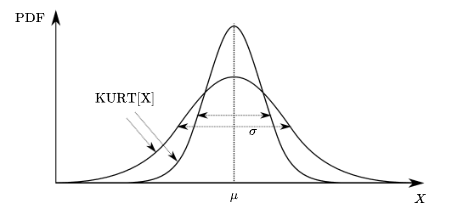
\includegraphics[width=250pt]{../img/01-moments.png}
        \caption{Figure 1.1: Variance and kurtosis}
    \end{center}
\end{figure}


\subsection{Skewness}

The third moment of statistics describes the symmetry of a distribution.

\[\bar \mu_3 = E\left[ \left( X - \mu \over \sigma \right)^3 \right] = {\mu_3 \over \sigma ^ 3}\]

Where \(\mu_3\) is the third central moment and \(\bar \mu_3\) is skewness or the third standardized central moment Positively skewed is called right skewed, because the long tail is on the right side. Similarly negatively skewed is left skewed.


\begin{figure}[htbp]
    \begin{center}
        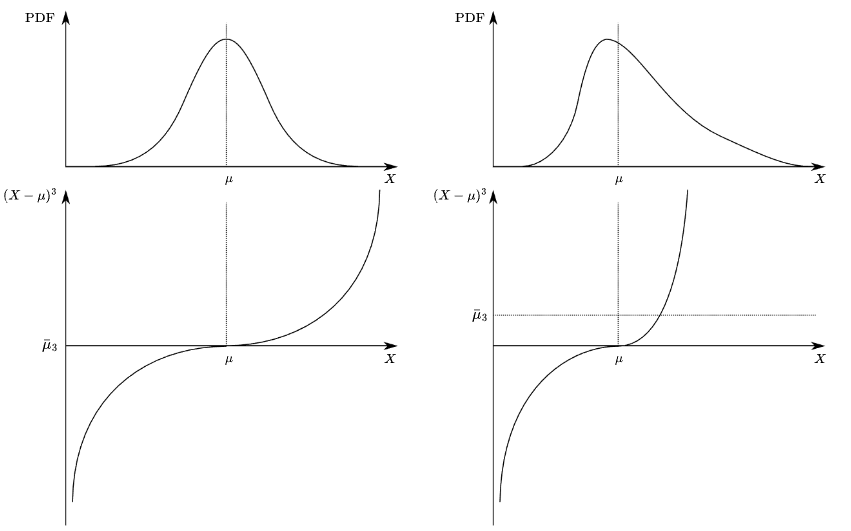
\includegraphics[width=350pt]{../img/01-skewness.png}
        \caption{Figure 1.2: Skewness}
    \end{center}
\end{figure}


To understand how the third power measures skewness, Figure 1.2 shows the third power of the normalized PDF. Values of \(X\) which are less than the mean is similar, but a right skewed distribution will have more points larger than the mean, the third power will grow faster, and the expectation of the third power will become positive.

Another method to measure skewness is using median and mode difference. Right skewed distribution will have mode smaller than the mean.

\section{Multiple random variables}

We sometimes want to work with multiple random variables.

\subsection{Joint probability distribution}

The joint probability of two variables is noted by

\[P(A, B) = P(A \cap B)\]

The joint probability distribution is

\[f(x, y) = P(X = x, Y= y)\]

We can write it in terms of conditional distribution

\[\begin{aligned}P(X,Y) &= P(X|Y)P(Y) = P(Y|X)P(X)\\
f(x, y) &= P(X = x | Y= y) \cdot P(Y= y) = P(Y = y | X = x) \cdot P(X = x)\end{aligned}\]

We can calculate the individual probability distributions from the joint probability distribution, and it's called the \textbf{marginal probability distributions\index{marginal probability distributions}} (if we enumerate a discreet joint probability distribution in a table, we would calculate the marginal distribution by summing up the rows and columns, making it the margin of the table as the last row and columns)

\[f_X(x) = \int f_{X,Y}(x,y)dy \\ f_Y(y) = \int f_{X,Y}(x,y)dx\]

Similarly to the probability distribution the joint cumulative distribution function

\[F_{X,Y}(x,y) = P(X \le x, Y \le y)\]

\subsection{Independent and identically distributed random variables (i.i.d)}

Two variables are \textbf{independent\index{independent}} when the conditional probability is same as the pior

\[P(A|B) = P(A)\]

The joint probability distribution for two independent variables becomes

\[P(A,B) = P(A)P(B)\]

Independence can be stated with cumulative distribution functions

\begin{equation}F_{X,Y}(x,y) = F_X(x)F_Y(y)\tag{i}\end{equation}

Two variables are \textbf{identically distributed\index{identically distributed}} if their joint cumulative distribution function is equal

\begin{equation}F_X(x) = F_Y(y)\tag{i.d}\end{equation}

Two variables are said to be \textbf{independent and identically distributed (i.i.d)\index{independent and identically distributed (i.i.d)}} if both condition for independence (eq. (i)) and identically distributed (eq. (i.d.)) are both satisfied.

\subsection{Covariance and correlation}

Similarity between two variables can be defined using correlation or covariance.

For a random sample covariance is defined as

\[\operatorname{Cov}(x,y) = \sigma_{xy} = {\sum(x - \bar x)(y - \bar y) \over n-1}\]

If X and Y have a relationship where Y grows when X does, the covariance will be positive. If Y has an opposite relationship, e.g. decreases as X increases, the Covariance is negative. If X and Y are independent, the Covariance is \(0\). Note that the opposite is not true, there might be a complex, non independent relationship between X and Y which would result in 0 Covariance.

For a discreet probability distribution covariance is

\[\operatorname{Cov}(X, Y) = \sum(X - E[X])(Y - E[Y])P(X,Y)\]

\textbf{Correlation\index{Correlation}} is defined as

\[\operatorname{Corr}(x,y) = {\sigma_{xy} \over \sigma_x \sigma_y}\]

Covariance can take up large values, while correlation is the normalized version of covariance, taking up values between \(-1\) and \(+1\) with the same meaning.

For a discreet probability distribution correlation is

\[\operatorname{Corr}(X, Y) = {\operatorname{Cov}(X, Y) \over \operatorname{SD}(X)\operatorname{SD}(Y)}\]

\subsection{Properties of expectation and variance}

Multiplying by a constant the expectation of a random variable gives

\[E[aX] = \int_{-\infty}^{\infty}aXf_XdX = aE[X] = a \mu_X\]

Similarly for variance, using the result we just got

\[Var(aX) = E[(aX - E(aX))^2] = E[(aX - aE(X))^2] = a^2 Var(X)\]

What these results show is that multiplying the random variable with a factor of \(a\), the mean will be scaled with same factor \(a\), but variance will be scaled with \(a^2\) because variance describes squared distance from the mean.

From the summation and integral properties we can easily show that the mean of a linear combination of two variables is a linear operation:

\[E[aX + bY] = aE[X] + bE[Y]\]

The variance of a linear combination is

\[Var(aX + bY) = a^2 Var(X) + b^2 Var(Y) + 2ab\operatorname{Cov}(X, Y)\]

If \(X\) and \(Y\) are independent variables, the \(\operatorname{Cov}\) term becomes \(0\), and we get

\[Var(aX + bY) = a^2 Var(X) + b^2 Var(Y)\]

Proof:
\begin{flalign*}
& Var(X) = E[(X - E[X])^2] \\
& =E[(aX + bY - E[aX + bY])^2] \\
& =E[(aX + bY - aE[X] - bE[Y])^2] \\
& =E[(aX - aE[X] + bY - bE[Y])^2] \\
& =E[(aX - aE[X])^2 + 2(aX - aE[X])(bY - bE[Y]) + (bY - bE[Y])^2] \\
& =E[a^2(X - E[X])^2 + 2ab(X - E[X])(Y - E[Y]) + b^2(Y - E[Y])^2] \\
& =E[a^2(X - E[X])^2] + E[2ab(X - E[X])(Y - E[Y])] + E[b^2(Y - E[Y])^2] \\
& \text{Finally using definition of variance and covariance, we get} \\
& =a^2 Var(X) + 2ab \operatorname{Cov}(X, Y) + b^2 Var(Y) \\ && \end{flalign*}

\chapter{Hypothesis testing}

Hypothesis testing is the process to confirm a test metric on a data set. The general process is to

\begin{enumerate}
    \item State a \textbf{null hypothesis\index{null hypothesis}} \(H_0\) which is the contradiction of the \textbf{alternative hypothesis\index{alternative hypothesis}} we want to verify, sometimes noted with \(H_1\)
    \item Use a \textbf{test statistic\index{test statistic}} to calculate the probability of an observation given the null hypothesis. This probability is the \textbf{p-value\index{p-value}}
    \item Compare the p-value to a target \(\alpha\) \textbf{significance level\index{significance level}}
\end{enumerate}

We say a null hypothesis is one tailed if

\[H_0: \mu = \mu_0,\ H_1 : \mu > \mu_0 \text{ or } H_1 : \mu < \mu_0\]

a two-tailed test is

\[H_0: \mu = \mu_0,\ H_1 : \mu \ne \mu_0\]

for some metric \(\mu\)

\section{Z-test and t-test}

\section{ANOVA}

ANOVA is used to verify means of multiple populations. If we apply Z-test multiple times, the error accumulates.

The ANOVA Hypothesis for \(p\) groups:

\[
\begin{aligned}
&H_0: \mu_1 = \mu_2 = ... = \mu_p,\  \\
&H_1: \mu_i \ne \mu_j,\ \forall i, j \in \{1, ...\ , p\}
\end{aligned}
\]



\chapter{Machine Learning}

In the world of data science there are two main views. From one side there is the mathematically well founded statistical methods like \textbf{statistical learning\index{statistical learning}} which mainly focuses on explaining population data from a sample. Various linear models are well defined within statistics. \textbf{Machine learning\index{Machine learning}} contains more complex techniques which might not have well founded probabilistic interpretations but provide good empirical results. There is major overlap and no easy way to differentiate the two views. We will start from statistical learning and move toward more complex machine learning models.

The most important building block of machine learning is the concept of a \textbf{model\index{model}}. A model is a series of assumptions or a simplified representation of a system. A model can be one or multiple mathematical equations, accompanied by a set of assumptions. The model might also be called a \textbf{data generator process\index{data generator process}} because based on the assumptions and simplifications it can generate new data with some error (see below).

In machine learning we try to fit a \textbf{model\index{model}} to a data set. There are two main objectives why we would like to do this:

\begin{itemize}
    \item \textbf{Inference\index{Inference}} about population properties by calculating the model properties.
    \item \textbf{Forecast\index{Forecast}} values of the population outside of the available sample/observations
\end{itemize}

The variable we would like to model or forecast is called the \textbf{dependent\index{dependent}} variable. The input variables used for modelling or forecast are called \textbf{independent\index{independent}} variables. We can model an \textbf{dependent\index{dependent}} \(Y\) variable with the \textbf{independent\index{independent}} variables \(X\) of a sample of observations. We assume the following relationship between the variables

\begin{equation}Y = f(X) + \epsilon \tag{4.1}\end{equation}

We define a model in the form

\begin{equation}\hat{Y} = \hat{f}(X) \tag{4.2}\end{equation}

\(\epsilon\) is the error term and can be decomposed using the expected value of (4.1) and (4.2) to two terms, called the \textbf{reducible error\index{reducible error}} and the \textbf{irreducible error\index{irreducible error}}:

\[E[(Y-\hat{Y})^2] = \underbrace{[f(X)-\hat{f}(X)]^2}_\text{Reducible error} + \underbrace{\text{Var}(\epsilon)}_\text{Irreducible error}\]

Proof:
\begin{flalign*}
& \text{Using (4.1) and (4.2)} \\
& E[(Y-\hat{Y})^2]=E[(f(X)+\epsilon-\hat{f}(X))^2] \\
& =E[(f(X)-\hat{f}(X))^2+2 \epsilon (f(X)-\hat{f}(X)) +\epsilon^2] \\
& \text{Because the expectation is linear operator} \\
& =E[(f(X)-\hat{f}(X))^2] +2E[\epsilon (f(X)-\hat{f}(X))] +E[\epsilon^2] \\
& \text{Because the expectation of} f \text{and} \hat{f} \text{are constant} \\
& =[f(X)-\hat{f}(X)]^2 +E[\epsilon^2] +2E[\epsilon (f(X)-\hat{f}(X)) \\
& \text{Because the mean of} \epsilon \text{is zero} \\
& =[f(X)-\hat{f}(X)]^2 +E[\epsilon^2] \\
& \text{Because the variance of} \epsilon \text{is} E(\epsilon^2) \\
& =[f(X)-\hat{f}(X)]^2 + \text{Var}(\epsilon) \\ && \end{flalign*}

We can optimize our model to minimize the reducible error but irreducible error is also unknown and our model might overfit by including some fit on the noise as well.

In many cases we need to assume casual relationship such as X causes Y, but in fact in some cases might be the opposite direction.

\section{Estimators}

An \textbf{estimator\index{estimator}} is a function of the data. It can either estimate parameters of the data directly or we can use it to estimate model parameters to find the best fit of the model to the data. Depending on the output of estimator we distinguish the following types of estimators:

\begin{itemize}
    \item \textbf{Point estimator\index{Point estimator}}: outputs a single value for a parameter. It is easy to interpret but might not give information on the variability or confidence.
    \item \textbf{Interval estimator\index{Interval estimator}}: outputs an interval providing insight to the confidence of the output.
    \item \textbf{Bayesian estimator\index{Bayesian estimator}}: outputs a probability distribution.
\end{itemize}

Given a population parameter \(\beta^P\), an estimator function \(\hat \beta\),and the samples \(S_1, S_2, ..., S_n\), we can apply the estimator function to each sample. This would result in a set of estimated parameters \(\beta^*_1, \beta^*_2, ..., \beta^*_n\)


\begin{figure}[htbp]
    \begin{center}
        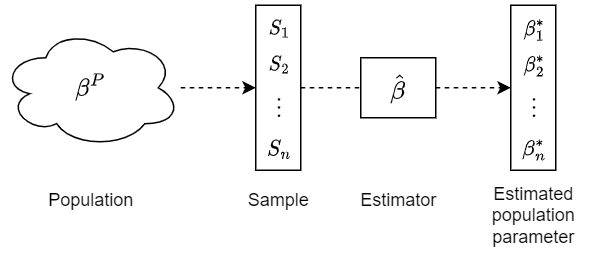
\includegraphics[width=250pt]{../img/03-estimator.png}
        \caption{Figure 3.1: Applying estimator to a set of observations}
    \end{center}
\end{figure}


Since the samples might not be fully representative of the population, the estimated parameters might also have some error to the real parameter \(\beta^P\).

If we calculate a property of multiple or all samples like the mean or variance these are also estimators for properties of the population.

We can define the following characteristics of an estimator

\begin{enumerate}
    \item \textbf{Unbiased\index{Unbiased}}: The expectation (mean) of the estimator matches the population parameter it estimates (see \textbf{Figure 3.2\index{Figure 3.2}} where the mean of the distribution is equal to the true population parameter)
\end{enumerate}

\[E[\hat \beta] = \beta^P\]

\begin{enumerate}
    \item \textbf{Consistent\index{Consistent}}: As the sample size grows, the estimator tends to the true value of the parameter (see \textbf{Figure 3.2\index{Figure 3.2}} where the red line is a small sample, the blue line is a larger sample and the green line would be an infinitely large sample or the entire population)
\end{enumerate}

\[n \to +\infty: \hat \beta \to \beta^P \]


\begin{figure}[htbp]
    \begin{center}
        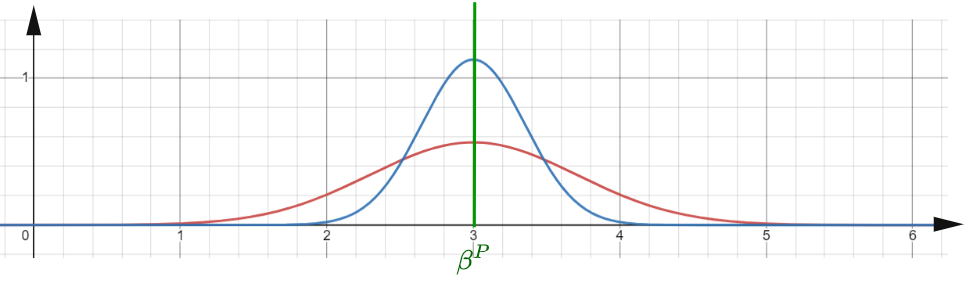
\includegraphics[width=250pt]{../img/03-estimate-distribution.png}
        \caption{Figure 3.2: <i>Plot of the probability distribution for the estimates which we get by applying an unbiased and consistent estimator to each sample. The red distribution is for a smaller sample with higher variance, the blue one is less variance measured on higher sample.</i>}
    \end{center}
\end{figure}


\textbf{Figure 3.3\index{Figure 3.3}} shows a biased but consistent estimator. For small sample sizes there is a bias between the true parameter and the mean of estimated parameters, but as the sample size increases, the distribution tends toward the true parameter.



\begin{figure}[htbp]
    \begin{center}
        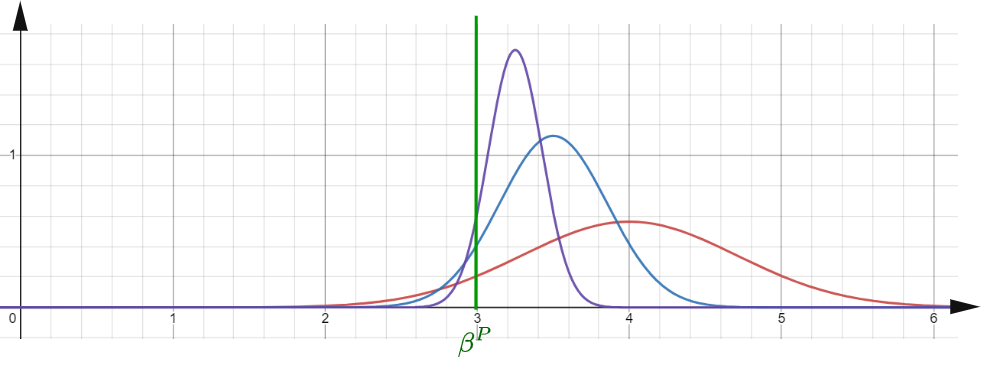
\includegraphics[width=250pt]{../img/03-biased-consistent-estimator.png}
        \caption{Figure 3.3: <i>Biased consistent estimator.</i>}
    \end{center}
\end{figure}



\begin{enumerate}
    \item \textbf{Efficiency\index{Efficiency}}: given two estimators \(\hat \beta\) and \(\widetilde \beta\), the estimator \(\widetilde \beta\) is said to be more efficient if it has lower variance using the same sample size. An efficient estimator might be biased. An example would be in \textbf{Figure 3.2\index{Figure 3.2}} if it were two different estimators with same sample size, one of them giving a more accurate distribution.
\end{enumerate}

\begin{enumerate}
    \item \textbf{Linear in parameters\index{Linear in parameters}} might be preferable so it can be mathematically easily manipulated.
\end{enumerate}

A specific case are the so called \textbf{BLUE estimators\index{BLUE estimators}} which stands for \textbf{best linear unbiased estimators\index{best linear unbiased estimators}}, meaning there is no better linear estimator available.

\section{Model fitting}

There are two main probabilistic optimization frameworks to estimate model parameters, also called \textbf{weights\index{weights}} in machine learning, given a set of observations: \textbf{Maximum Likelihood Estimation\index{Maximum Likelihood Estimation}} (MLE) and \textbf{Maximum a Posteriori\index{Maximum a Posteriori}} (MAP). The difference is that MAP assumes a prior probability distribution and tries to estimate parameters using the posterior probability, MLE estimates parameters using the prior based on observations only.

\[\theta_{MLE} = argmax_{\theta}\ f_n(x_1...x_n|\theta)\]

If values of \(x_1...x_n\) are i.i.d or we assume it, becomes

\[\theta_{MLE} = argmax_{\theta}\ \prod_{i=1}^nf(x_i|\theta)\]

We than try to optimize \(L(\theta)\). Since it's an optimization problem, we can optimize log likelihood of \(log\ L(\theta)\) instead to facilitate derivative calculations and avoid underflow due to several products of small decimal values.

If we assume a prior distribution in addition to our observations, we can apply MAP, which maximizes the posterior function :

\[
\begin{aligned}
\theta_{MAP} &= argmax_{\theta}\ f(\theta|x_1...x_n) \\
&= argmax_{\theta}\ g(\theta) f(x_1...x_n|\theta)
\end{aligned}
\]

We skipped the denominator (so-called marginal likelihood) after applying the Bayes rule above because it does not change the optimization problem.

For example for linear regression, MLE estimates the mean squared loss, applying MAP will estimate L2 regularization as well.

There are two main methods of model fitting
\begin{itemize}
    \item If there is closed solution for the optimization we can apply analytical calculation. This is only possible in few cases, for simple models with few parameters
    \item Iterative approach: a more commonly used approach, which can fit very complex models
\end{itemize}

\section{Cost function and bias-variance trade-off}

To measure how well the model fits our observed data we can use a \textbf{cost function\index{cost function}}. For a function to be considered as a cost function, it needs to fulfill the following attributes

\begin{itemize}
    \item Should always be positive
    \item If our estimate improves, the cost function should decrease
\end{itemize}

Using the likelihood function, which is the probability we can observe our data given our model, we can transform it to be a positive function, which decreases the better the fit. This is called the \textbf{negative log likelihood cost function\index{negative log likelihood cost function}}. Given a set of observations \(X\) and a statistical model with parameters \(\theta\) and the likelihood \(L(\theta | X)\), the cost function is:

\[\operatorname{NLL} = - \ln(L(\theta | X))\]

This equation looks scary, but likelihood is basically the probability of observing the data given the model parameters. The logarithms is used because it provides several computational benefits:

\begin{itemize}
    \item Since probabilities are usually small numbers. When multiplied together, as in the case of joint probabilities for sequences, they can become extremely small and lead to underflow issues in computers (since computers can store numbers up to some precision, the value might become smaller than this precision, leading to instability).
    \item In many cases, especially when working with likelihoods, products of probabilities get converted to sums when we take the logarithm. This transformation simplifies the computations and makes them more efficient. For example \(\log(p_1  p_2) = \log(p_1) + \log(p_2)\)
\end{itemize}

The likelihood function is mainly used to estimate parameters of probability distribution given the observed data, but might not have closed form or might have more than one local minima which is why other cost functions which are easier to optimize might be used to fit machine learning models.

A popular example of a cost function is the \textbf{mean squared error\index{mean squared error}} or MSE, which is the average of the squared difference of predicted and actual output for each observation \(i\).

\[\operatorname{MSE} = {1 \over n} \sum_{i=1}^n(y_i - \hat{f}(x_i))^2 \]

The MSE of an estimator \(\hat{\theta}\) with respect to an unknown parameter \(\theta\) is defined as

\[\operatorname{MSE}(\hat\theta)=E_\theta[ ({\hat \theta}-\theta )^{2} ]\]

MSE can be decomposed to a combination of bias and variance of the estimator

\[{\displaystyle \operatorname {MSE} ({\hat \theta})=\operatorname {Var} _\theta({\hat \theta})+\operatorname {Bias} ({\hat \theta},\theta )^{2}}\]

Proof

Using the definition of variance
<!--mleq-->
\(\operatorname{Var}(X) = E(X^{2}) - (E(X))^{2}\) \\
\(E(X^{2})=\operatorname{Var}(X)+(E(X))^{2}\)

By substituting \(X\) with \(\hat {\theta }-\theta\) it can be shown that

\(\operatorname{MSE} ({\hat {\theta }})=\mathbb {E} [({\hat {\theta }}-\theta )^{2}]\)\\
\(=\operatorname {Var} ({\hat {\theta }}-\theta )+(\mathbb {E} [{\hat {\theta }}-\theta ])^{2}\)\\
\(=\operatorname {Var} ({\hat {\theta }})+\operatorname {Bias} ^{2}({\hat {\theta }})\)
<!--mleq-->

Variance is always positive and bias is squared. The selected estimator needs to minimize either of or both of variance and bias in order to minimize \(\operatorname{MSE}\)

We can scale MSE to be the same size as our data, this metric is called \textbf{Root Mean Square Error\index{Root Mean Square Error}} or RMSE

\[\operatorname{RMSE} = \sqrt{\operatorname{MSE}}\]

For other cost functions we don't have a neat mathematical decomposition like with MSE, we still observe a tradeoff. For various other loss functions, the essence of the bias-variance tradeoff still exists. Whether we are using cross entropy for logistic regression, or custom loss functions for other models, the fundamental tension between fitting the training data well (and risking overfitting) versus generalizing to new data (and risking underfitting) remains. A model with too many parameters might overfit the training data and perform poorly on new, unseen data (high variance, low bias). Conversely, an overly simple model might not capture the underlying patterns in the training data, leading to systematic errors (high bias, low variance).

\section{Regularization}

\section{Model selection}

When we would like to fit a model to the data. We first assume a model structure, this process is called \textbf{model selection\index{model selection}} e.g. a linear model, tree model, neural network, etc. Many of the models have some assumptions about the data we try to fit the model to. We need to consider or verify these assumptions. When selecting a model we also consider difficulty of building. Some models can be created more easily (e.g linear models, tree models) compared to others which require more work (neural network).

Once we selected our model, we proceed to estimate the model parameters. There are two main types of model parameters:
\begin{itemize}
    \item \textbf{Weights\index{Weights}} or \textbf{parameters\index{parameters}}: are function parameters we can adjusted during the learning process to best fit the model to the observed data.
    \item \textbf{Hyperparameters\index{Hyperparameters}}: describe the structure of model or method of model fitting, e.g. learning rate, layers in a neural network, the K in KNN, etc
\end{itemize}

The methods of estimating weights and the methods of finding the right hyperparameters are different.

\section{Model validation}

Cross validation
Goodness of fit

\section{Hyper parameter tuning}


\chapter{Linear Regression}

\textbf{Linear models\index{Linear models}} are a set of supervised statistical learning techniques, used to approximate an unknown function based on observations using a liner combination of predictors and weights.

Linear regression tries to map continuous or categorical variables to a continuous independent variable. For \(x_1...x_p\) predictor variables and \(\epsilon\) irreducible error term, linear regression model has the form

\[y = \beta _0 + \beta _1 x_1 + ... + \beta _p x_p + \epsilon\]

The regression coefficients \(\beta_1...\beta_p\) are unknown, an estimate takes the form

\[\hat y = \hat \beta _0 + \hat \beta _1 x_1 + ... +  \hat \beta _p x_p\]

\(\epsilon\) is the error term. For a linear fit, the error term is assumed to be independent and identically distributed with mean 0 and constant variance:

\[\epsilon \sim i.i.d(0, \sigma^2)\]

Independent means that the error of a sample does not give information about the error of an another sample. Identically distributed means errors come from the same distribution. For example the error does not depend of \(x\).


\begin{figure}[htbp]
    \begin{center}
        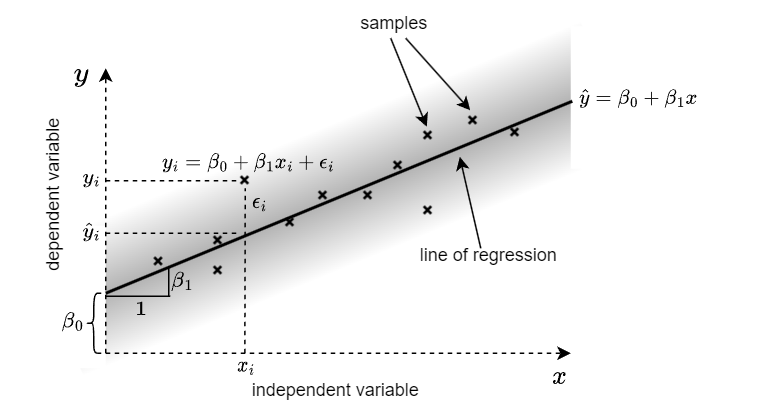
\includegraphics[width=200pt]{../img/04-linear-regression.png}
        \caption{Figure 4.1: Linear regression with a single predictor, called simple linear regression. The gray shading represents the error distribution around the linear regression.}
    \end{center}
\end{figure}


\section{Fitting the model}

Linear regression has a closed form solution so we can derive the best fit line analytically. Parameters can be estimated using our training data set and the sum of squared residual loss function

\[\operatorname{RSS} = \sum_{i=1}^n(y_i - \hat y)^2 = \sum_{i = 1}^n \hat\epsilon_i^2\]

As a matrix representation, we can write our linear regression as:

\[\begin{pmatrix} y_1 \\ y_2 \\ \vdots \\ y_n \end{pmatrix} =
 \begin{pmatrix}
  x_{1,1} & x_{1,2} & \cdots & x_{1,p} \\
  x_{2,1} & x_{2,2} & \cdots & x_{2,p} \\
  \vdots  & \vdots  & \ddots & \vdots  \\
  x_{n,1} & x_{n,2} & \cdots & x_{n,p}
 \end{pmatrix}
 \begin{pmatrix} \beta_1 \\ \beta_2 \\ \vdots \\ \beta_p \end{pmatrix} + \begin{pmatrix} \epsilon_1 \\ \epsilon_2 \\ \vdots \\ \epsilon_n \end{pmatrix}\]

Or simply as

\[Y = X \beta + \epsilon\]

where \(n\) is the number of samples, \(p\) is the number of predictors, and \(\epsilon\) is the error. We don't know the real weights and error term, so we use hat notation for estimates as

\begin{equation}Y = X \hat\beta + \hat\epsilon \tag{4.1}\end{equation}

We can write \(\operatorname{RSS}\) as

\(\operatorname{RSS} = \sum_{i = 1}^n \hat\epsilon_i^2 = \begin{pmatrix} \hat\epsilon_1 & \hat\epsilon_2 & \cdots & \hat\epsilon_n \end{pmatrix} \begin{pmatrix} \hat\epsilon_1 \\ \hat\epsilon_2 \\ \vdots \\ \hat\epsilon_n \end{pmatrix} = \hat\epsilon^T\hat\epsilon\)\\

From rearranging (4.1) and plugging in we get\\
\(\operatorname{RSS} = (Y-\hat\beta X)^T(Y-\hat\beta X)\)

Because the transpose operator \(A^T\) is a linear operator, we can apply to each item individually (we also need to change order of matrix multiplication):

\begin{flalign*}
& \operatorname{RSS} = (Y^T- X^T \hat\beta^T)(Y-\hat\beta X) \\
& \operatorname{RSS} = Y^T Y - Y^T \hat\beta X - X^T \hat\beta^T Y + X^T \hat\beta^T \hat\beta X \text{We would like choose} \hat\beta \text{which minimizes} \operatorname{RSS} \text{, i.e:} argmin_{\hat\beta} \operatorname{RSS} \text{. For this we can calculate} \beta \text{for which the derivate is} 0 \text{:} \\
& {\partial \operatorname{RSS} \over \partial \hat\beta} = 0 \\
& {\partial \over \partial \hat\beta}(Y^T Y - Y^T \hat\beta X - X^T \hat\beta^T Y + X^T \hat\beta^T \hat\beta X) = 0 \\
&  \\ && \end{flalign*}

The first term is \(0\), the second term is the transpose of the third. Notice that all terms results in a scalar, but the gradient results in a column vector, so result has to be the \(0\) column vector, which we can notate as \(O\).

\begin{flalign*}
& -X^T Y - X^T Y + 2 X^T X \hat\beta = O \\
& \text{We can rearrange as} \\
& 2 X^T X \hat\beta = 2X^T Y \\
&  \\ && \end{flalign*}

We can remove the \(2\) and multiply both side by \((X^TX)^{-1}\), which cancels out on the left, resulting in

\[\hat\beta = (X^TX)^{-1} X^T Y\]

To be able to derive \(\hat\beta\), the term \(X^TX\) needs to be invertible, so it has to be non singular (determinant is non 0). An example for singular case is when there is perfect colliniarity between two or more predictors.

\section{Assess quality of fit}

To assess quality of fit, the \textbf{residual standard error\index{residual standard error}} \(RSE\) is an estimate of standard deviation of \(\epsilon\)

\[\operatorname{RSE} = \sqrt{\operatorname{RSS} \over n - p - 1}\]

\(RSE\) is on same scale as \(y\), \(R^2\) is another measure of fit on the scale between \(0\) and \(1\)

\[
\begin{aligned}
R^2 &= {\operatorname{variance\ explained} \over \operatorname{total\ variance}} = {Var(\operatorname{mean}) - Var(\operatorname{fit}) \over Var(\operatorname{mean})}
\\
&= {{\operatorname{TSS} \over n} - {\operatorname{RSS} \over n} \over {\operatorname{TSS} \over n}} = {\operatorname{TSS} - \operatorname{RSS} \over \operatorname{TSS}} = 1 - {\operatorname{RSS} \over \operatorname{TSS}}
\end{aligned}
\]

where \(TSS\) is \textbf{total sum of squares\index{total sum of squares}}: \(TSS = \sum(y_i - \bar y)^2\). \(\bar y\) is the average of \(y\). \(RSS\) is the amount of variability unexplained after regression, \(TSS\) is the total variability. Some text books use this notation

\[R^2 = {SS(\operatorname{mean}) - SS(\operatorname{fit}) \over SS(\operatorname{mean})} \]

In simple liner regression setting (\(y = \beta _0 + \beta _1 x\)), \(R^2\) is same as \(\operatorname{Corr}(X, Y)^2\)

If we have \(p+1\) observations \(R^2\) will \textit{*}always be \(1\)\textit{*} because we are fitting a \(p\) dimensional plane on \(p+1\) points so there is always a perfect fit. Such a fit however has very little confidence. To calculate p-value for \(R^2\) we use the \(F\) value

\[F = {\operatorname{variance\ explained} \over \operatorname{variance\ not\ explained}} = {SS(\operatorname{mean}) - SS(\operatorname{fit}) / (p_{\operatorname{fit}} - p_{\operatorname{mean}}) \over SS(\operatorname{fit}) / (n - p_{\operatorname{fit}})}\]

Where in case of linear regression \(p_{\operatorname{mean}}\) is \(1\)

We can either simulate lots of \(F\) scores by sampling our data, calculating the fitted line and \(F\) score and finally calculating the \(F\) score for the whole dataset and finding percentiles of more extreme values from our simulations, or we can use the \textit{F*}-distribution

\section{Categorical predictors}

Categorical predictors can be added trough dummy encoding. In this case the equation will be

\[y = \beta_0 + \sum_{c \in C}\beta_cx_c\]

Where \(C\) contains all categorical values except one which will act as baseline (and be part of intercept). If all dummies are included, it will cause multi colliniarity because the last dummy explains the others.

\section{Extensions to the linear model}

We can remove additive assumptions by creating custom predictors combining other predictors called \textbf{interactions\index{interactions}} or adding \textbf{polynomial terms\index{polynomial terms}} . E.g.

\[y = \beta_0 + \beta_1x_1 + \beta_2x_2 + \beta_3x_1x_2 + \beta_4x_2^2 + \beta_5x_2^3\]

When we include interactions or polynomial terms we should always include the base predictors called \textbf{main effects\index{main effects}}. Categorical variables only contribute to intercept, to add slope effect as well, needs to be added to interaction

\section{Assumptions of linear regression}

The \textbf{Gauss-Markov theorem\index{Gauss-Markov theorem}} proposed by two mathematicians says that ordinary least squares is the best linear unbiased estimator (BLUE) under the following assumptions:

\begin{enumerate}
    \item \textbf{Linear in parameters\index{Linear in parameters}}: coefficients of the predictors must be linear. For example \(\beta_0 + \beta_1X_1 + \epsilon\) is linear but \(\beta_0 + \beta_0\beta_1X_1 + \epsilon\) is not. Can be verified using residual plots (\(e_i = y_i - \hat y_i\) vs \(x_i\) or in the case of multiple regression \(y_i\)). In case of non linearity polynomial terms can be used, e.g \(\beta_0 + \beta_1X_1 + \beta_2X_1^2\) and similar exponential terms are still linear in parameters.

    \item \textbf{Random sampling\index{Random sampling}}: our samples \(\{x_i, y_i\}\) are randomly selected from a population. This assumption also contains the assumption that all samples come from the same population.

    \item \textbf{No perfect colliniarity\index{No perfect colliniarity}} in regressors: there cannot be an exact relationship between regressors. \textbf{Multicolliniarity\index{Multicolliniarity}} happens if there is correlation between predictor variables. If two predictors are correlated, increasing the coefficient of one can be cancelled out by a corresponding opposite change of the other coefficient, thus making coefficients highly unstable (multiple values for coefficients result in same fit, including infinitely large coefficients). Pairwise correlation can be detected by plotting the correlation matrix of the predictors. Can be quantified trough the \textbf{variance inflation factor\index{variance inflation factor}} (VIF) \[\operatorname{VIF}(\beta_j) = {1 \over 1 - R_{X_jX-j}^2}\].

    \item \textbf{Zero conditional mean\index{Zero conditional mean}} of error: \[E(\epsilon | X) = 0\] means the expectation of the error term does not depend on the value of x. The error is uniformly distributed along the regression line (does not move above or below the line depending on the value of X). It's also called \textbf{exogeneity\index{exogeneity}}, which means there is no hidden variable or relationship influencing the error term. If there is a relationship and violates this assumption, we say the regressor is influenced by or are \textbf{endogenous\index{endogenous}} to the error term (endogeneity).

    \item \textbf{Constant variance of error terms\index{Constant variance of error terms}} or \textbf{homoscedastic errors\index{homoscedastic errors}}: if error terms increase with dependent variable, it's called \textbf{heteroscedasticity\index{heteroscedasticity}} and can be seen on the residual plot as a funnel shape. In the case of this issue, we can transform the response using a concave function (\(\sqrt{y}\) or \(log(y)\)). Another option might be to fit using \textbf{weighted least squares\index{weighted least squares}}.

\begin{figure}[htbp]
    \begin{center}
        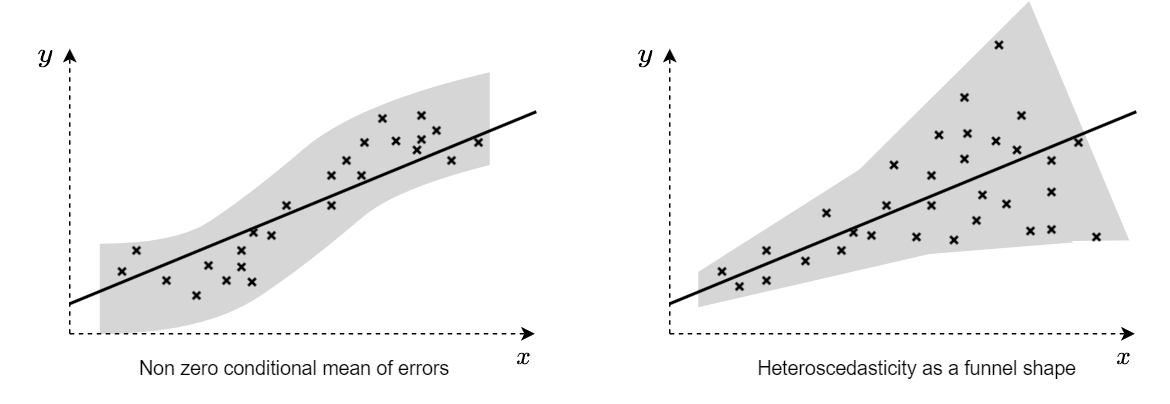
\includegraphics[width=300pt]{../img/04-assumptions.png}
        \caption{Figure 4.2: Non zero conditional mean on left, error are below or above the line as X changes and heteroscedastic errors on the right.}
    \end{center}
\end{figure}


    \item \textbf{Error terms are uncorrelated\index{Error terms are uncorrelated}}, an error term \(\epsilon_i\) provides no information about \(\epsilon_j\), like sign or distance, which is the case for example for time series analysis. Mathematically this can be expressed as \[Cov(\epsilon_i, \epsilon_j) = 0 \implies i = j\]
\end{enumerate}

\section{Other considerations}

\subsection{Outliers}

\textbf{Outliers\index{Outliers}} can be identified from residual plot, or we can plot \textbf{studentized residuals\index{studentized residuals}} \[\bigg|{\epsilon_i \over SE}\bigg| > 3\] \\
Outliers might indicate incorrect data input in which case can be simply removed or issues with model like missing predictor variable

\subsection{High leverage points}

\textbf{High leverage points\index{High leverage points}}  are observations which have unusual predictor \(x_i\) values and might easily influence the regression. A so called \textbf{leverage statistic\index{leverage statistic}} can be calculated to quantify leverage, more so for multiple predictors


where \(R_{X_jX-j}^2\) is the \(R^2\) of a regression of \(X_j\) to the other predictors. Minimum value for VIF is 1, a value above 5 or 10 indicated multicolliniarity.
In case of multicolliniarity we can remove one of the predictors or combine multiple predictors into one.

Interactions and polynomial terms can cause multicolliniarity for non centered predictors, centering solves this issue, see [here](https://stats.stackexchange.com/questions/60476/collinearity-diagnostics-problematic-only-when-the-interaction-term-is-included).

\section{K-Nearest Neighbor regression}

KNN is a non parametric estimator, and so does not make assumptions about the form of \(f(X)\). On the other hand, does not support inference (explaining predictor relationships). To perform KNN regression, we find the K nearest neighbors of \(x_0\) noted with \(N_0\), and we calculate the average of training responses

\[f(x_0) = {1 \over K} \sum_{x_i \in N_0}y_i\]

A parametric approach usually outperforms the non parametric one, because the non parametric can have an increase in variance without reducing bias. With large number of predictors, the \textbf{curse of dimensionality\index{curse of dimensionality}} reduces the number of neighbors that can be used. In some cases KNN might perform better, but model expandability and the presence of p-values are advantages of linear regression.

\chapter{Linear Models for Classification}

Classification is the problem of mapping variables to a categorical dependent variable. While in some cases there can be more than two categories, we can reduce the problem of classifying to a category or another and repeating for the latter.

We can measure performance of classifier trough the error rate

\[{1 \over n} \sum_{i=1}^nI(y_i \ne \hat y_i)\]

where \(\hat y\) is predicted class for \(i\) th observation and \(I(y_i \ne \hat y_i)\) is an indicator having value of \(0\) in case of misclassification and \(1\) for correct classification.

The test error rate is minimized by maximizing the \textbf{Bayes classifier\index{Bayes classifier}}, which assigns each observation to the most likely class, given the value \(x_0\) of the predictor variable \(X\).

\begin{equation}argmax_j(P(Y = j | X = x_0))\tag{5.1}\end{equation}

We use \(argmax\), because we need the \(j\) class for the maximum probability and not the maximum probability itself.

Prediction of the Bayes classifier is determined by the so called \textbf{Bayesian decision boundary\index{Bayesian decision boundary}} where probability is \(0.5\). The Bayes classifier produces the lowest error rate called \textbf{Bayes error rate\index{Bayes error rate}}, which is the expectation of the error term over all values of \(X\)

\[1 - E[argmax_j(P(Y = j | X))]\]

The Bayes error rate is analogous to the irreducible error of linear models. The Bayes classifier in most cases is unknown and we would like to estimate it.

Proofs:
https://en.wikipedia.org/wiki/Bayes\_classifier

Same as regression there are two main categories of classification: non parametric like KNN and parametric classification.

Parametric classifications can be further categorized based on the parameter estimation approach (see also \textbf{Figure 5.1\index{Figure 5.1}}):
\begin{itemize}
    \item \textbf{Discriminative classifier\index{Discriminative classifier}}: we estimate probability of an observation to belonging to a particular value of categorical variable \(Y\), drawing a separation boundary. Example: logistic regression.
    \item \textbf{Generative classifier\index{Generative classifier}} we estimate distribution of each class of \(Y\) separately based on observations and using all estimates of an observation, we choose the maximum to decide final class. Examples:
    \item Naive Bayes
    \item Linear discriminant analysis (LDA), a dimensionality reduction technique
    \item Quadratic discriminant analysis
    \item Hidden Markov Model
\end{itemize}


\begin{figure}[htbp]
    \begin{center}
        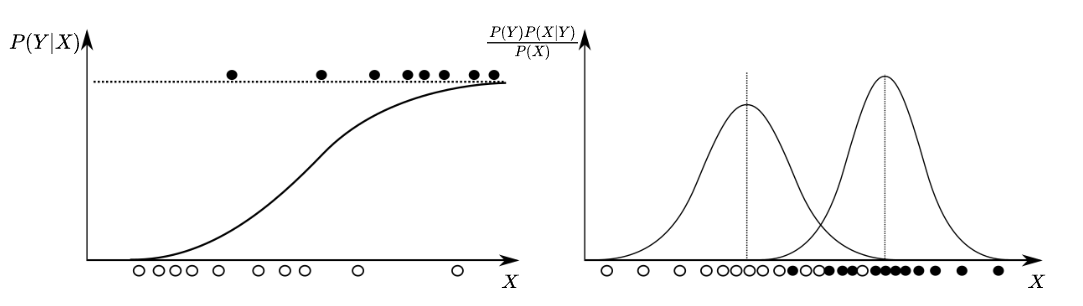
\includegraphics[width=300pt]{../img/05-discriminative-generative.png}
        \caption{Figure 5.1: <i>Discriminative (left) vs generative (right) classifier</i>}
    \end{center}
\end{figure}


\section{K nearest neighbor classifier (KNN)}

KNN classifier tries to estimate the Bayes classifier, by finding the K nearest observation in training data closest to \(x_0\) test observation

\[P(Y = j | X = x_0) = {1 \over K} \sum_{i \in N_0}I(y_j = j)\]

The classifier result will be the class \(j\) of the maximum probability: \(argmax_j(P)\)

\[C^{KNN}(x) = argmax_j({1 \over K} \sum_{i \in N_0}I(y_j = j))\]

Small K values lead to higher variance, \(K=1\) will perfectly fit the training data.

\section{Logistic regression}

In logistic regression we model the probability of an observation belonging to one of two classes with logistic function. Output ranges between 0 and 1 (<b>Figure 5.2</b> left side)

\[P(X) = {e^{\beta_0 + \beta_1X_1 + ... +  \beta_pX_p} \over 1 + e^{\beta_0 + \beta_1X_1 + ... + \beta_pX_p}}\]

We can transform the above to odds form \(p \over 1-p\)

\begin{flalign*}
& P(X) = {e^z \over 1 + e^z} \\
& P(X)\cdot(1 + e^z) = e^z \\
& P(X) + P(X) e^z = e^z \\
& P(X) = e^z(1-P(X)) \\
& {P(X) \over 1 - P(X)} = e^z \\ && \end{flalign*}

Giving

\[{P(X) \over 1 - P(X)} = e^{\beta_0 + \beta_1X_1 + ... + \beta_pX_p}\]

Taking \(log\) of both sides gives the log odds or \textbf{logit\index{logit}}

\[log\bigg({P(X) \over 1 - P(X)}\bigg) = \beta_0 + \beta_1X_1 + ... + \beta_pX_p\]

Which is a linear function, see right side of \textbf{Figure 5.2\index{Figure 5.2}}


\begin{figure}[htbp]
    \begin{center}
        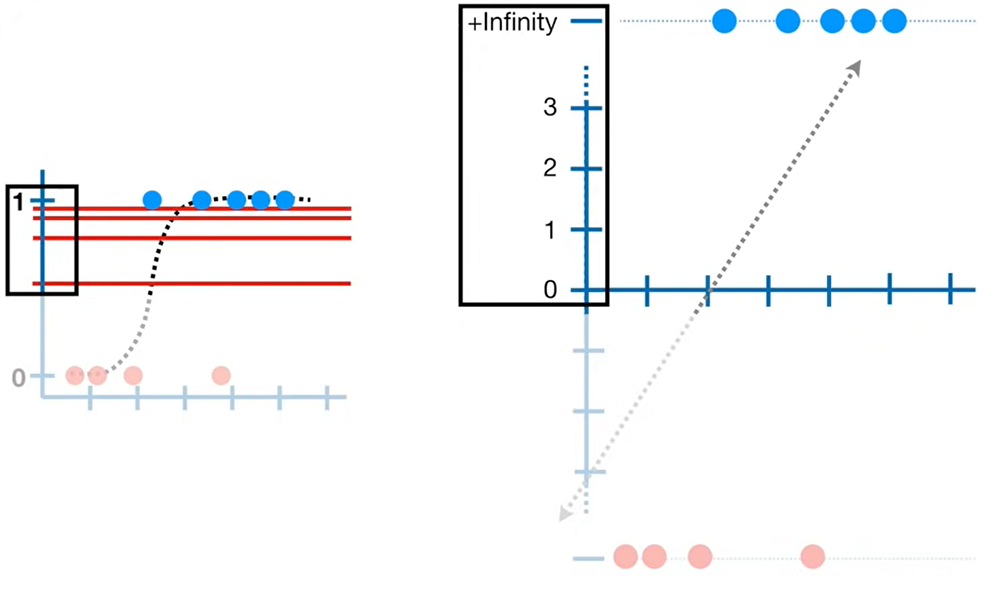
\includegraphics[width=200pt]{../img/05-log-function.png}
        \caption{Figure 5.2: <i>Left side probability p, rights side logit transformation. Observations move from 0 to negative infinity and from 1 to infinity</i> (source StatQuest)}
    \end{center}
\end{figure}


We can use categorical variables trough dummies, same as linear regression.

\subsection{Fitting the model}

The logistic function can be fit using maximum likelihood. The likelihood function is

\[\ell(\beta_0, \beta_1) = \prod_{i:y_i=1}p(x_i)\prod_{j:y_j=1}\big (1 - p(x_j)\big )\]

\subsection{Multinomial logistic regression}

Multinomial logistic regression is used to classify more than two classes. To achieve this we use a reference class and coefficients tell the relative change of one class probability compared to another.

Model for classifying multiple classes when using the \(K\) th class as reference for classes \(k = 1...K-1\)

\[P(Y=k|X=x) = {e^{\beta_{k0} + \beta_{k1}X_1 + ... + \beta_{kp}X_p} \over 1 + \sum_{l=1}^{K-1}e^{\beta_{l0} + \beta_{l1}X_1 + ... + \beta_{lp}X_p}}\]

and for class \(K\)

\[P(Y=K|X=x) = {1 \over 1 + \sum_{l=1}^{K-1}e^{\beta_{l0} + \beta_{l1}X_1 + ... + \beta_{lp}X_p}}\]

we can derive

\[log\bigg({P(Y=k|X=x) \over P(Y=K|X=x)}\bigg)=\beta_{k0} + \beta_{k1}X_1 + ... + \beta_{kp}X_p\]

Proof (with simplified notations):

\(log\big({P(k) \over P(K)}\big) = log\bigg({{e^{z_k} \over 1 + \sum_{l=1}^{K-1}e^{z_l}} \over {1 \over 1 + \sum_{l=1}^{K-1}e^{z_l}}}\bigg) = log({e^{z_k} \over 1}) = log(e^{z_k}) = z_k\)

An alternative is to use softmax encoding, we estimate coefficients for all classes \(k = 1...K\)

\[P(Y=k|X=x) = {e^{\beta_{k0} + \beta_{k1}X_1 + ... + \beta_{kp}X_p} \over \sum_{l=1}^K e^{\beta_{l0} + \beta_{l1}X_1 + ... + \beta_{lp}X_p}}\]

and we calculate ration between classes \(k\) and \(k'\)

\[log\bigg({P(Y=k|X=x) \over P(Y=K|X=x)}\bigg)=(\beta_{k0}-\beta_{k'0}) + (\beta_{k1}-\beta_{k'1})X_1 + ... + (\beta_{kp}-\beta_{k'p})X_p\]

Proof (with simplified notations):

\(log\big({P(k) \over P(k')}\big) = log\big({e^{z_k} \over e^{z_{k'}}}\big) = log(e^{z_k}) - log(e^{z_{k'}}) = z_k - z_{k'}\)

\subsection{Assessing the model}

Each estimated coefficient has associated \textit{z*}-statistic
\[\hat \beta_1 \over \operatorname{SE}(\hat \beta_1)\]

If \textit{z*}-statistic is large, and the associated \(p\)-value is below a selected \(\alpha\) we can reject the null hypothesis: \(H_0: \beta_1 = 0\)

\section{Generative Models for Classification}

Instead of directly estimating \(P(Y = y|X = x)\) we estimate the distribution \(P(X|Y=k)\) for each value \(k\) of \(Y\) and then we use Bayes rule to flip the conditional and calculate \(P(Y = y|X = x)\).

If \(P(Y = k)\) is the overall probability that an observation belongs to class \(k\) (i.e \(n_k \over n\) where \(n_k\) is samples in class \(k\) and \(n\) is total number of samples of our training data) and \(P(X | Y = k)\) is the distribution of a single class, using Bayes rule we get

\begin{equation}P(Y = k|X = x) = {P(Y = k) P(X = x | Y = k) \over \sum_{l=1}^K P(Y = l) P(X = x | Y = l)}\tag{5.2}\end{equation}

The denominator makes sure the resulting probability distribution sums to \(1\).

Benefits of generative models over logistic regression:

\begin{itemize}
    \item Can be easily applied to more then two class in the output
    \item If separation of classes is more prominent, generative models are more stable.
\end{itemize}

The challenge is to estimate the distribution of samples within each class \(P(X = x | Y = k)\), for which techniques such as linear discriminant analysis or naive bayes can be used, described below.

\subsection{Linear discriminant analysis}



\subsection{Naive Bayes classifier}

In case of the Naive Bayes classifier we make the assumption that within the class \(k\) of \(Y\), the predictor variables are independent:

\begin{equation}P(X = x | Y = k) = \prod _{j}P(X_j = x_j | Y = k)\tag{5.3}\end{equation}

Where \(X_1, ..., X_p\) are the predictor variables, and \(x_1, ..., x_p\) are values of an observation (the one we are classifying) for each predictor. While in most cases the predictor variables are not independent, estimating the covariance between all combinations of predictor variables is very difficult. With this assumption, some bias is introduced in favour of reducing variance (we reduce model parameters, see bias-variance trade off). If we plug in equation (5.3) to (5.2) and the result to (5.1) we get the following result:

\[{\displaystyle C^{\text{Bayes}}(x)={\underset {k}{\operatorname {argmax} }}\operatorname {P} (Y=k)\prod _{j} P(X_j = x_j|Y=k)}\]

Complete breakdown for reference

\begin{flalign*}
& \displaystyle C^{\text{Bayes}}(x)=argmax_k(P(Y = k | X = x)) \\
& \text{Plugging in (5.2) but notating the denominator with} \alpha \text{for simplicity} \displaystyle C^{\text{Bayes}}(x)=argmax_k \biggl( {P(Y = k) P(X = x | Y = k) \over \alpha} \biggr) \\
& \text{Since} \alpha \text{is positive and constant for all terms, it will not change the outcome of} argmax \text{, we caan simply omit} \\
& \displaystyle C^{\text{Bayes}}(x)=argmax_k \bigl( P(Y = k) P(X = x | Y = k) \bigr) \\
& \text{Finally we plug in the (5.3) assumption} \\
& \displaystyle C^{\text{Bayes}}(x)=argmax_k \bigl( P(Y = k) \prod _{j}P(X_j = x_j | Y = k)] \bigr) \\
&  \\ && \end{flalign*}

To complete the classification task, estimating \(P(X_j = x_j|Y=k)\) for each predictor \(X_1, ..., X_j\) is remaining. There are a few ways to achieve this.

\begin{itemize}
    \item If \(X_j\) is quantitative, we can assume \(P(X_j|Y = k)\) to be normally distributed, in this case we can follow the same process as QDA, with an added assumption that the covariance matrix of each class is diagonal
    \item An alternative in case of a quantitative \(X_j\) is to use a kernel density estimator or simply create a histogram from the training data, normalize it so the sum of bins is \(1\) and use the bin height for \(x_0\) (see Quantitative predictor on Figure 5.3).
    \item For a qualitative \(X_j\) we can follow a similar process to the histogram one: count all training observation for each class. The resulting probability \(P(X_j = x_j|Y=k)\) is the ratio of the occurrences of \(x_0\) in the training data for the class \(k\) to the total number of training samples occurring for the class \(k\) (see Qualitative predictor Figure 5.3).
\end{itemize}


\begin{figure}[htbp]
    \begin{center}
        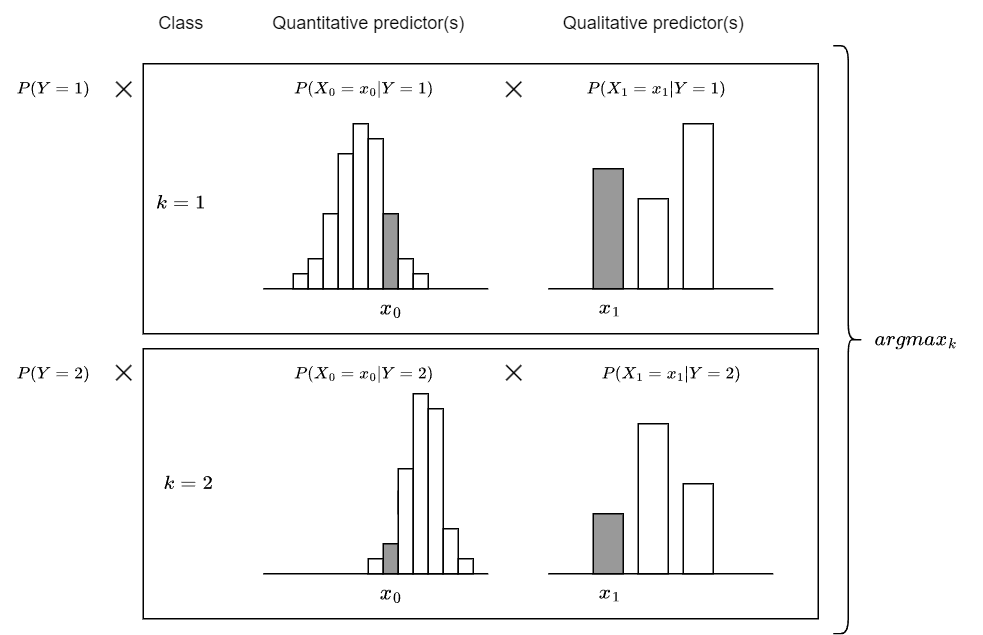
\includegraphics[width=300pt]{../img/05-naive-bayes.png}
        \caption{Figure 5.3:  Naive bayes classifier. For each class we calculate the product of the probability of the input of all predictors independently, finally choose the class with highest probability.}
    \end{center}
\end{figure}


\section{Evaluating classifiers}

<table>
  <tr>
    <td colspan="2" rowspan="2"></td>
    <th align="center" colspan="2">Predicted class</th>
    <td rowspan="2"></td>
  </tr>
  <tr>
    <th align="center">Positive</th>
    <th align="center">Negative</th>
  </tr>
  <tr>
    <th rowspan="2">Actual class</th>
    <th align="center">Positive</td>
    <td align="center">True Positive (TP)</td>
    <td align="center">False Negative (FN)\\<span style="color: \#ff5555">Type II error</span></td>
    <td align="center"><b>Sensitivity or Recall</b> \[TP \over TP + FN\]</td>
  </tr>
  <tr>
    <th align="center">Negative</td>
    <td align="center">False Positive (FP)\\<span style="color: \#ff5555">Type I error</span></td>
    <td align="center">True Negative (TN)</td>
    <td align="center"><b>Specificity</b> \[TN \over TN + FP\]</td>
  </tr>
  <tr>
    <td colspan="2"></td>
    <td align="center"><b>Precision</b> \[TP \over TP + FP\]</td>
    <td colspan="2"></td>
  </tr>
</table>



\chapter{Decision trees}

Decision tree based models have reduced utility in terms of inference but are good at forecasting. An important metric used for tree growing, more so for classification is

\chapter{Feed forward networks}

\section{Perceptron}

The building block of a neural network is the \textbf{perceptron\index{perceptron}} which is a mathematical model of a biological neuron, or brain cell. Similar to how neurons have dendrids, a perceptron has inputs and an \textbf{activation function\index{activation function}}. The inputs are fed in as a linear combination, with each input being assigned a weight. Weights are usually real numbers.


\begin{figure}[htbp]
    \begin{center}
        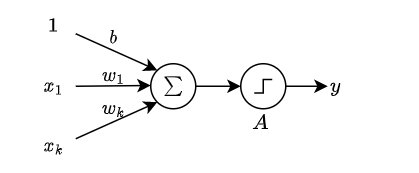
\includegraphics[width=150pt]{../img/07-perceptron.png}
        \caption{Figure 7.1: Model of a neuron}
    \end{center}
\end{figure}


We can model the combination of inputs and weights as a dot product. The threshold of activation or \textbf{bias\index{bias}} of the perceptron is modelled with an added input \(1\) and a weight noted with \(b\). The dot product becomes \(z = b + w \cdot x = b + \sum_j w_jx_j\).

For the neural network to be able to approximate any function, needs to non linear. Since inputss and weights are linear combination, this non liniarity is achieved trough the activation function which in most cases is not linear.

Neural networks use various functions as activation functions:


\begin{figure}[htbp]
    \begin{center}
        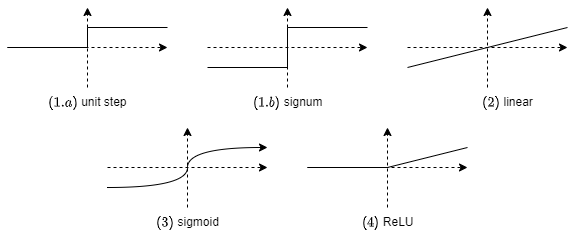
\includegraphics[width=300pt]{../img/07-activation-functions.png}
        \caption{Figure 7.4: Activation functions}
    \end{center}
\end{figure}


\begin{enumerate}
    \item \textbf{Step function\index{Step function}}: can be either unit step

\[h = \begin{cases}
0 & \operatorname{if }\ z > 0 \\
1 & \operatorname{if }\ z \le 0
\end{cases}
\]

or signum, where \(-1\) is used instead of \(0\). The challenge with this is that small change in the input might trigger a jump from \(0\) to \(1\) times weights, which might be a sudden big jump and if organized to network it might not learn.

    \item \textbf{Linear\index{Linear}}

\[h = z \]

Same as linear regression. In case multiple neurons are connected will still collapse to linear model. To be able to model non linear functions, the activation should also be non linear

    \item \textbf{Sigmoid\index{Sigmoid}}

\[h = {1 \over 1 + e^{-z}}\]

Small changes in the input will result in small changes in the output because the function is continuous.

\[\Delta h \approx \sum_j {\partial h \over \partial w_j} \Delta w_j \]

Sigmoid can become saturated on values close to \(0\) (low) and \(1\) (high) because the derivate becomes close to \(0\).

    \item \textbf{Rectifier Linear Unit: ReLU\index{Rectifier Linear Unit: ReLU}}

\[h = max(0, z)\]

A variant is the \textbf{leaky ReLU\index{leaky ReLU}} which allows small negative values to be passed trough. It:s defined as

\[h = max(az, z)\]

where \(a\) is a very small constant (e.g. \(0.0001\)). While the rectified unit is not continuous and it has some issues like vanishing or exploding gradient in learning, it's still very popular due to it's simplicity and good performance in practice if used as part of large neural networks.
\end{enumerate}

\section{Network structure}

In feed forward networks, output of neurons in a layer act as inputs in the next layer


\begin{figure}[htbp]
    \begin{center}
        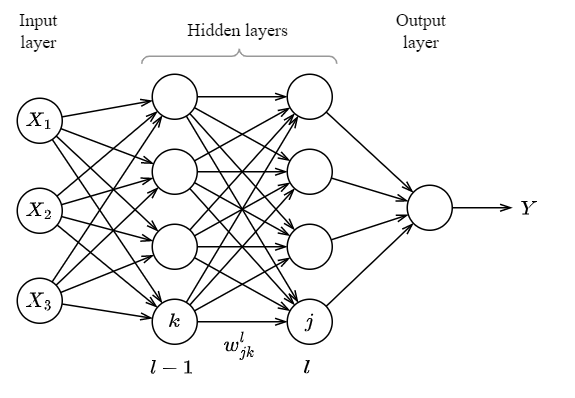
\includegraphics[width=287pt]{../img/07-feedforward-network.png}
        \caption{Figure 7.3: Architecture of a feed forward neural network with 3 inputs and 2 hidden layers}
    \end{center}
\end{figure}


To train the model we can choose a loss function \(C\) we could minimize. To minimize \(C\) we can define a change in \(C\) as the sum of all partial derivates of \(C\) over all the weights \(w_k\)

\begin{equation}\Delta C \approx \sum_k { \partial C \over \partial w_k} \Delta w_k = \nabla C \Delta w_k \tag{7.1}\end{equation}

\(\nabla C\) (pronounced nabla) is simply a notation for the sum of partial derivates. We can make a decrease in the cost function \(C\) by choosing \(\Delta w_k\) as

\[\Delta w_k = -\eta \nabla C\]

Where \(\eta\) is the learning rate. Plugging it to (7.1) we get

\[\Delta C \approx - \eta \| \nabla C \| ^ 2\]

Since \(\| \nabla C \| ^ 2\) is positive, \(- \eta\) is negative, so will always result in moving in direction of decrease in \(\Delta C\). The update rule of weights to minimize the cost function \(C\) is

\begin{equation}w_k' = w_k - \eta { \partial C \over \partial w_k}\tag{7.2}\end{equation}

Similarly we can write the same for bias as well

\begin{equation}b' = b - \eta { \partial C \over \partial b}\tag{7.3}\end{equation}

\subsection{Cost functions}

The MSE seen in Chapter 3 is often used with ReLU but does not work well with sigmoid neurons or if the output layer is a softmax layer (see below).

If the neuron is saturated on the opposite value which it has to learn, adjusting from one side to another will require many learning iterations, the initial learning rate being very slow (until the learning gets to the steep part of the sigmoid function). Because of this limitation, a better alternative to be used with sigmoid is the \textbf{cross entropy cost function\index{cross entropy cost function}}

\begin{equation}C = -{1 \over n}\sum_x[y \ln a + (1 - y) \ln (1-a)] \tag{7.5}\end{equation}

Cross entropy definition relates to entropy in information theory (see \#todo under trees): cross entropy measures the \textit{s}urprise\textit{ }when we learn the true probability \(y\) for a predicted probability \(a\) as \(H(y,a) = -\sum_xy_i\log_2(a_i)\), using natural log \(\ln\) instead of \(\log\), which is same from optimization perspective (ratio is a constant of \(\ln 2\)). (7.5) is a special case of cross entropy also called \textbf{binary cross entropy\index{binary cross entropy}} (we will refer to it simply as cross entropy cost function), which has two terms to penalize prediction of true label if actual label is false and also penalize prediction of false label when actual label is true.

Cross entropy cost function acts as a cost function because it's always positive (both terms in the sum are negative for \(a \in [0, 1]\) making overall result positive) and for small differences between \(y\) and \(a\), will result in a small result as cost.

To see why this seemingly complex function is useful, we could check the learning rate for a single sigmoid neuron, notated with \(\sigma(z)\) the partial derivate against a weight \(w\):

\({\partial C \over \partial w_j} = {\partial \over \partial w_j }{\big ( -{1 \over n}\sum_x(y \ln \sigma(z) + (1 - y) \ln (1-\sigma(z)))\big ) }\)

\(= -{1 \over n}\sum_x \left ( {\partial \over \partial w_j}\big ( y \ln \sigma(z)\big ) + {\partial \over \partial w_j} \big ((1 - y) \ln (1-\sigma(z))\big )\right )\)

Because \(ln(x)' = {1 \over x}\)

\({\partial C \over \partial w_j} = -{1 \over n}\sum_x \left ( {y \over \sigma(z) } {\partial \sigma(z) \over \partial w_j} - {1 - y \over 1-\sigma(z)} {\partial \sigma(z) \over \partial w_j}\right )\)

Notice how the sign in the middle flipped because of \(ln'(1-\sigma(z))\)

\({\partial C \over \partial w_j} = -{1 \over n}\sum_x \left ( {y \over \sigma(z) } - {1 - y \over 1-\sigma(z)}\right ) {\partial \sigma(z) \over \partial w_j} \)

Since \(z = b + \sum_j x_jw_j\) the derivate will be \({\partial \sigma(z) \over \partial w_j} = \sigma'(z) z'(w_j) = \sigma'(z) x_j\), pluggin in

\({\partial C \over \partial w_j} = -{1 \over n}\sum_x \left ( {y \over \sigma(z) } - {1 - y \over 1-\sigma(z)}\right ) \sigma'(z)x_j\)

We can rewrite \({y \over \sigma(z) } - {1 - y \over 1-\sigma(z)} = {y(1-\sigma(z)) - (1 - y)\sigma(z) \over \sigma(z) (1-\sigma(z)) } = {y - \sigma(z) - y\sigma(z) + y\sigma(z) \over \sigma(z) (1-\sigma(z))} = {y - \sigma(z) \over \sigma(z) (1-\sigma(z))}\). We get

\({\partial C \over \partial w_j} = -{1 \over n}\sum_x \left ( {y - \sigma(z) \over \sigma(z) (1-\sigma(z))}\right ) \sigma'(z)x_j\)

Using the definition of sigmoid \(\sigma(z) = {1 \over 1 + e^{-z}}\), and the rule \(\left( 1 \over f \right )' = (f^{-1})' = -f^{-2} f'\) we can calculate\\

\(\sigma'(z) = \left (-{1 \over ( 1 + e^{-z})^2} \right ) e^{-z} (-1)\) \\
\(= {e^{-z} \over ( 1 + e^{-z})^2 } = {1 \over  1 + e^{-z}} {e^{-z} \over 1 + e^{-z}} = {1 \over  1 + e^{-z}} {1 + e^{-z} - 1 \over 1 + e^{-z}} = {1 \over 1 + e^{-z}} \left ( 1 - {1 \over  1 + e^{-z}} \right ) \)\\
\(= \sigma(z)(1 - \sigma(z))\). \\
Plugging the result, i.e \(\sigma'(z) = \sigma(z)(1 - \sigma(z))\) to \({\partial C \over \partial w_j}\) will give

\({\partial C \over \partial w_j} = -{1 \over n}\sum_x \left ( {y - \sigma(z) \over \sigma(z) (1-\sigma(z))}\right ) \sigma(z)(1 - \sigma(z)) x_j \)\\
\(= -{1 \over n}\sum_x(y - \sigma(z))x_j\)

\[{\partial C \over \partial w_j} = {1 \over n}\sum_x(\sigma(z) - y)x_j\]

The result shows that the learning rate \({\partial C \over \partial w_j}\) is proportional to the difference between expected and actual output \(y - \sigma(z)\). The larger the difference the better the learning rate. The same is not true if we use MSE with sigmoid.

We can claculate the same for bias the only difference is \({\partial \sigma(z) \over \partial b} = \sigma'(z) z'(b) = \sigma'(z)\), resulting in

\[{\partial C \over \partial b} = {1 \over n}\sum_x(\sigma(z) - y)\]

Cross entropy giving a simple result when calculating gradients makes it a good choice to improve the learning rate.

Less popular but the negative log likelyhood function might also be used with softmax output.

\section{How networks learn}

Training neural networks can be highly inefficient so we need various optimizations. First we optimize on how we use the input data. To calculate the rate of change in cost function (7.4) or (7.5) we could iterates trough all input data, but this process would be costly. Instead of calculating the change in cost function for all inputs, we can select a subset of size \(m\) of training data, noted with \(X_j\), called \textbf{mini batch\index{mini batch}} to update the weights. The update would take the form

\[w_k' = w_k - {\eta \over m} { \partial C_{X_j} \over \partial w_k} \]

In some cases the \(1 \over m\), which scales the learning rate with batch size, can be ommitted. A complete iteration over all training data trough batches is called an \textbf{epoch\index{epoch}}.

Trough the example of cross entropy, we looked at how a single neuron learns but calculating the same way how an entire network learns is not efficient. All forward paths would need to be distangled and summed up several times. It would basically mean recalculating every subtree every time it shows up after a perceptron as we step trough the graph. Instead more efficient algorithms can be used which move backward, reusing already computed results.

\textbf{Backprograpagation\index{Backprograpagation}} is the algorithm used in training, specifically for calculating \(\partial C \over \partial w\)  and \(\partial C \over \partial b\) from equations (7.2) and (7.3) respectively for a multi layer neural network.

\subsection{Assumptions of backpropagatation}

\begin{enumerate}
    \item The cost function \(C\) can be written as the average of the cost function for all training samples \(x\) noted \(C_x\). This assumption is needed because backpropagation is done per training sample
\end{enumerate}

\[C = {1 \over n} C_x\]

\begin{enumerate}
    \item The cost function can be written as a function of the outputs of the network. Having \(L\) as the number of layers
\end{enumerate}

\[C = C(A^L)\]

\textbf{Notations\index{Notations}}

\begin{itemize}
    \item \(w_{jk}^l\) as the weight from \(k\) th neuron in \(l-1\) th layer to \(j\) neuron in \(l\) th layer (figure 7.5)
    \item \(b_j^l\) is bias of the \(j\) th neuron in layer \(l\)
    \item \(h\) activation method used
    \item \(A_j^l\) is activation of the \(j\) th neuron in layer \(l\)
\end{itemize}

   The activation function

   \[A_j^l = h(b_j^l + \sum_k w_{jk}^l A_j^{l-1})\]

Transforming to matrix form

\begin{itemize}
    \item \(w^l\) is the weight matrix of layer \(l\) where columns are  \(k\) (\(l-1\) layer neuron) and rown are \(j\) (\(l\) layer neuron) for weight \(w_{jk}^l\)
    \item \(b^l\) bias vector
    \item Applying a function to a vector is equivalent of applying to all vector elements: \(h(z)_j \equiv h(z_j)\)
    \item \(A^l\) activation vector becomes\[A^l = h(z^l) = h(b^l + w^l A^{l-1})\] The reversal of order of \(j\) and \(k\) in \(w_{jk}^l\) is to eliminate the transpose \(w^T\) of weight matrix \(w\) in the above equation.
    \item Hadaman product is the element wise product of two vectors resulting in a vector, noted with \(\odot\) \[(s \odot t)_j = s_j t_j\]
\end{itemize}


\subsection{ Equations of backpropagation}

Backpropagation is an algorithm to calculate \({\partial C \over \partial w^l}\) and \({\partial C \over \partial b^l}\), by introducing an error term in the \(j\) th neuron noted with \(\delta_j^l\)

By making a weighted input change of a neuron \(\Delta z_j^l\), this would cause the output of neuron to be \(h(z_j^l + \Delta z_j^l)\), overall cost would change \({\partial C \over \partial z_j^l} \Delta z_j^l\). To minimize cost, we can choose \(\Delta z_j^l\) to be \(- {\partial C \over \partial z_j^l}\), so that it would result in a minus squared term which is always negative, and thus would help us reduce the cost function. Thus the error term we can choose is

\begin{equation}\delta_j^l = {\partial C \over \partial z_j^l} \tag{7.6}\end{equation}

The vector \(e^l\) is the error term for layer \(l\).

\textbf{Error in out payer\index{Error in out payer}} (element wise and matrix form):

\[\delta_j^L = {\partial C \over \partial A_j ^ L} h ' (z_j^L)\]

\begin{equation}\delta^L = \nabla _AC \odot h(z^L) \tag{BP1}\end{equation}

Proof:

\begin{flalign*}
& \text{Start with (7.6)} \\
& \delta_j^l = {\partial C \over \partial z_j^l} \\
& \text{applying the chain rule} \\
& \delta_j^l = \sum_k{\partial C \over \partial A^L_k}{\partial A^L_k \over \partial z_j^l} \\
& \text{Since activation} A \text{of} k \text{th neuron depends only of the weighted input of the same neuron} z \text{we can eliminate all terms where} k \ne j \\
& \delta_j^l = {\partial C \over \partial A^L_j}{\partial A^L_j \over \partial z_j^l} \\
& \text{Because by definition} A^L_j = h(z_j^L) \text{we can rewrite the second term} \\
& \delta_j^l = {\partial C \over \partial A^L_j}h'(z_j^L) \\
&  \\ && \end{flalign*}

\textit{*}Error of layer \(l\) in respect to error in laer \(l+1\)\textit{*}

\begin{equation}\delta^l = \big ((w^{l+1})^T \delta^{l+1}\big ) \odot h(z^l) \tag{BP2}\end{equation}

The first half moves the error backward a layer, the second half, moves error trough the layer

(BP1) and (BP2) allow calculating the error \(e\) for all layers

Proof:

\begin{flalign*}
& \text{Start with (7.6)} \\
& \delta_j^l = {\partial C \over \partial z_j^l} \\
& \text{applying the chain rule, in terms of} \\
& \delta_j^{l+1} = {\partial C \over \partial z_j^{l+1}} \\
& \text{we get} \\
& \delta_j^l = \sum_k{\partial C \over \partial z_j^{l+1}}{\partial z_j^{l+1} \over \partial z_j^l} \\
& \delta_j^l = \sum_k{\partial z_j^{l+1} \over \partial z_j^l}\delta_k^{l+1} \\
& \text{The first term} \\
& {\partial z_j^{l+1} \over \partial z_j^l} = {\partial \sum_j w_{kj}^{l+1} f(z_j^l) + b_k^{l+1} \over \partial z_j^l} = w_{kj}^{l+1}h'(z_j^l) \\
& \text{Adding it back} \\
& \delta_j^l = \sum_k w_{kj}^{l+1} \delta_k^{l+1} h'(z_j^l) \\
& \text{Writing the same in matrix form we get} \\
& \delta^l = \big ((w^{l+1})^T \delta^{l+1}\big ) \odot h(z^l) \\ && \end{flalign*}

\textbf{Rate of change of cost in respect to bias\index{Rate of change of cost in respect to bias}}

\begin{equation}{\partial C \over \partial b^l} = \delta^l \tag{BP3}\end{equation}

Proof:

\begin{flalign*}
& {\partial C \over \partial b^l} = \sum_k {\partial C \over \partial z_k^l}{\partial z_k^l \over \partial b_j^l} \\
& \text{Since} z_k^l \text{only dependson on} b_j^l \text{where} k = j \\
& {\partial C \over \partial b^l} = {\partial C \over \partial z_j^l}{\partial z_j^l \over \partial b_j^l} = \delta^l{\partial z_j^l \over \partial b_j^l} \\
& {\partial C \over \partial b^l} = \delta^l{\partial \sum_j w_{kj}^l f(z_j^{l-1}) + b_k^l \over \partial b_j^l} \\
& \text{The second term is simply} 1 \text{resulting in} \\
& {\partial C \over \partial b^l} = \delta^l \\ && \end{flalign*}

\textbf{Rate of change of cost in respect to weights\index{Rate of change of cost in respect to weights}}

\begin{equation}{\partial C \over \partial w^l} = A^{l-1}\delta^l \tag{BP4}\end{equation}

Proof

\({\partial C \over \partial w^l} = \sum_m {\partial C \over \partial z_m^l}{\partial z_m^l \over \partial w_{kj}^l}\)

\({\partial C \over \partial w^l} = \sum_m {\partial C \over \partial z_m^l}{\partial \sum_n w_{mn}^lA_n^{l-1} + b_m^l \over \partial w_{kj}^l}\)

and only when \(m = j\) and \(n = k\), the derivative is not \(0\), so here we get

\({\partial C \over \partial w_{jk}^l} = {\partial C \over \partial z_j^l}A_k^{l-1} = A^{l-1}\delta^l\)

\subsection{Algorithm of backpropagation}

The algorithm (using mini batches)

\begin{enumerate}
    \item For each input of a mini batch \(x\), use as \(A^1\) of input layer
            \begin{enumerate}
            \item Feed forward trough layers \(l = 2, 3, ..., +L\) with \(z^l = w^lA^{l-1} + b^l\) and \({A^l} = h(z^l)\)
            \item Calculate output error with (BP1)
            \item Backpropagate error with (BP2)
        \end{enumerate}
    \item Adjust weights and biases with learning rate times the average of gradients given by (BP3) and (BP4)
\end{enumerate}

The reason backpropagation is faster than forward learning is because we would need to compute the gradient for all combinations of weights for each layer. Since most of the computation is redundant in the sense that partial gradients are recalculated multiple times, for each forward path, the backpropagation algoroithm optimizes on this to compute only once.

\section{Techniques used to improve learning}

In recent years a number of techniques has been developed to improve the performance of neural networks

\subsection{Softmax output layer}

Softmax can be used with both ReLU and sigmoid activation functions, but works best with the cross entropy cost function. The softmax is similar to a multi variate logistic regression. We apply it to the last layer of the network only, noted with \(L\)

\[A_j^L = {e^{z_j^L} \over \sum_k e^{z_k^L}}\]

The output of softmax normalizes all outcomes to always sum up to \(1\).

\[\sum_k A_k^L = {\sum_k e^{z_k^L} \over \sum_k e^{z_k^L}} = 1\]

The output is always positive since \(e^x\) is always positive. These two propoerties make the softmax function a probability distribution, which means we can treat the output of a network as an estimated probibility for each classification.

\section{References}

\textbf{An Introduction to Statistical Learning, with applications in R, Second Edition\index{An Introduction to Statistical Learning, with applications in R, Second Edition}}, Gareth James, Daniela Witten, Trevor Hastie, Rob Tibshirani

\textbf{Neural Networks and Deep Learning\index{Neural Networks and Deep Learning}}, Michael Nielsen 2019


\chapter{Dimensionality reduction}

Supervised machine learning models in most cases require that training data or sample size \(n\) is much greater than the number of predictors or features \(p\)

\[n \gg p\]

Linear models will have high variance and overfit data as \(p\) gets closer to \(n\). If \(p = n\), ordinary least squares linear regression will perfectly fit the data, and will perform poorly an a test set.

Adding features as dimensions to a linear model will increase \(R^2\) even though the model fit quality decreases. \(R^2\) can be adjusted to number of features. It is defined as:

\[R^2_{adj} = 1 - {(n-1)RSS \over (n - p - 1)TSS}\]

WIth each added dimension, the data sparsity increases exponentially, because the volume of the data hypercube also increases exponentially. This is called the \textbf{curse of dimensionality\index{curse of dimensionality}}. Dimensionality reduction techniques help reduce the dimensionality of features while preserving as much as possible about the data conveyed.

Dimensionality reduction can be performed directly on a dataset or on a model. A number of techniques have been proposed to reduce dimensionality ranging from linear techniques to neural network based techniques.

\section{Dimensionality reduction of linear models}

Linear dimensionality reduction methods can transform a linear model to a lower number of predictors by substituting to another smaller set of predictors.

Let the following be a linear model

\[Y = \beta_0 + \sum_{i=1}^p\beta_iX_i\]

Where \(Y\) and \(X_i\) are a vector of size \(n\), where \(n\) is the sample size. We can define a linear transformation to a lower dimension \(M\), as

\[Z_m = \sum_{j=1}^p \phi_{jm}X_j\]

where \(M<p\) and \(m = 1,...,M\) and \(\phi_{jm}\) are the parameters for dimensionality reduction. We can rewrite our model with the new parameters \(Z_m\) as:

\[Y = \theta_0 + \sum_{m=1}^M\theta_mZ_m\]

We can fit this model with less parameter: \(M + 1\), compared to \(p + 1\), where \(M < p\). We can fit the model with ordinary least squares in the same way we would fit the original model. It's called dimensionality reduction, because we reduced the number of model parameters.

The relationship between the model parameters are:

\[\beta_j = \sum_{m = 1}^M\theta_m \phi_{jm}\]

So far we omitted the task on choosing the \(\phi_{jm}\) parameters. Depending on how we choose them, OLS on the reduced model might provide a better fit. Linear dimensionality techniques can be used to reduce both the data directly as well as the linear models.

\section{Principal Component Analysis}

\textbf{Principal Component Analysis\index{Principal Component Analysis}} (PCA) is a form of \textbf{unsupervised learning\index{unsupervised learning}}, which means no labeled training dataset is needed. PCA can be used to reduce the dimension of an \(n \times p\) matrix.

The PCA method remaps the basis vectors of the dataset (in Figure 8.1 the basis vectors are unit vectors on the axis \(X_1\) and \(X_2\) respectively). The first principal component we choose in PCA is the one where the variance of the data is maximum (in Figure 8.1 the diagonal continuous line). Projecting the observations to the line of the first principal component results in the largest variance of the projected data, compared to any other line. In other words, the first principal component is the line closest to the data.


\begin{figure}[htbp]
    \begin{center}
        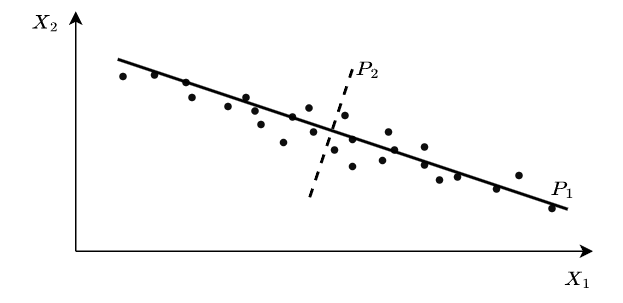
\includegraphics[width=250pt]{../img/08-principal-component.png}
        \caption{Figure 8.1:  Principal components of a two dimensional dataset}
    \end{center}
\end{figure}


Since in the example there is high correlation between \(X_1\) and \(X_2\), the first principal component captures this relationship. The second component is chosen to capture the remaining maximum variance, in this case the remaining variance. Principal components are uncorrelated, so they are perpendicular to one another.

When we have \(p\) features, we can choose in similar manner up to \(p\) principal components. Since we maximize capturing variance with each component we can limit the number of components to \(M\), where \(M < p\), resulting in dimensionality reduction, while still minimizing data loss.

To compute the principal components we use spectral decomposition. For a full treatment on linear algebra, eigenvalues, eigenvectors and matrix decomposition, see Appendix II. For a data matrix \(X\) (where each row is an observation and columns are the features \(X_1, ..., X_n\)) the algorithm for PCA is as follows:

\begin{enumerate}
    \item \textbf{Center the Data\index{Center the Data}}: Before PCA is applied, the data is usually centered. This means subtracting the mean of each feature from the data so that the mean of the centered data is zero.
    \item \textbf{Compute the Covariance Matrix\index{Compute the Covariance Matrix}}: For the centered data matrix \(X\), compute the covariance matrix \(\Sigma\) given by: \[\Sigma = \frac{1}{n-1} X^T X\] Where \(n\) is the number of observations.
    \item \textbf{Spectral decomposition of the Covariance Matrix\index{Spectral decomposition of the Covariance Matrix}}: Compute the eigenvectors and eigenvalues of the covariance matrix \(\Omega\). Since \(\Omega\) is the form of \(X^T X\) scaled by a constant, means it's a symmetric matrix, which in turn means that its eigenvectors are orthogonal, and can be decomposed using spectral decomposition. Let \(V\) be the matrix whose columns are the eigenvectors of \(\Sigma\) and \(\lambda\) be the corresponding eigenvalues. Using spectral decomposition will have the form of:
\[\Omega = V \Sigma V^T \]
    \item \textbf{Order the Eigenvectors\index{Order the Eigenvectors}}: Sort the eigenvectors in \(V \) in descending order based on the magnitude of their corresponding eigenvalues in \(\Sigma\). The reason for this is that the largest eigenvalue corresponds to the direction of the greatest variance in the data, the second largest to the second most direction of variance, and so on.
    \item \textbf{Principal Components\index{Principal Components}}: The sorted eigenvectors are the principal components. They provide an orthogonal basis for the data space, with each component capturing a descending amount of the total variance in the data. These are the first \(k\) columns of \(V\), noted with \(V_k\).
    \item \textbf{Projection\index{Projection}}: The original data \(X\) can be projected onto these top \(k\) principal components (or right singular vectors) using:
\end{enumerate}

\[X_k=XV_k\]

The principal components essentially provide a new coordinate system for the data where the axes are aligned with the directions of maximum variance (as determined by the eigenvectors of the covariance matrix). By ordering these axes by the amount of variance they capture (as determined by the eigenvalues), we can efficiently reduce the dimensionality of the data, if desired, by only considering the most significant axes.

\section{Autoencoders}



\chapter{Time series analysis and forecasting}

In this chapter we will explore time series analysis and forecasting techniques. We will start with linear models and move on to more complex ones.

In \textbf{time series\index{time series}} data we don't really have a population, instead we have a data generating process, that we are sampling at certain points in time. Population would mean all observations at any given time, which would mean an infinite number of observations.


\begin{figure}[htbp]
    \begin{center}
        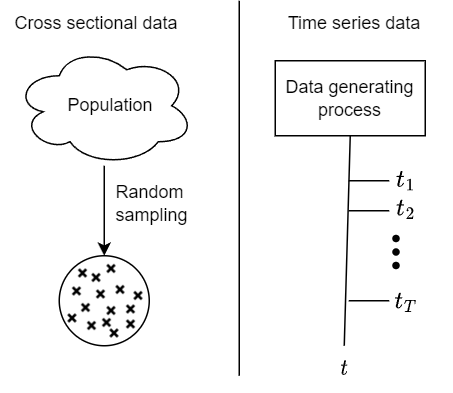
\includegraphics[width=250pt]{../img/09-time-series.png}
        \caption{Figure 9.1:  Cross sectional data (left) vs time series data (right)}
    \end{center}
\end{figure}


\section{Linear models for time series analysis}

In the case of linear regression, the Gauss-Markov conditions are required for OLS to provide the best linear unbiased estimator (BLUE). However, for time series analysis, other linear models may be more appropriate.

\subsection{Assumption of linear models for time series}

Time series linear models require some modifications to the Gauss-Markov assumptions, such as the inclusion of strict exogeneity instead of weak exogeneity. Nevertheless, in practice, when the sample size is large enough, similar conditions apply.

In cross-sectional data analysis, the assumption is that the samples are independent and identically distributed (i.i.d). However, in time series analysis, the assumption of independence no longer holds due to temporal dependence between the observations. Instead of assuming i.i.d, we introduce the concept of \textbf{weak dependence\index{weak dependence}}.

A time series is considered weakly dependent if the correlation between a value and a lagged value tends to zero as the lag tends to infinity:
\[Corr(x_t, x_{t+h}) \rightarrow 0, h \rightarrow \infty\]

This condition serves as a replacement for the random sampling assumption in cross-sectional data. Since the correlation becomes minimal as the lag increases, we can treat the observations as if they were i.i.d, allowing us to perform inference.

Some of the linear models we can use for time series require that the time series is \textbf{stationary\index{stationary}}. The conditions for stationary time series are

\begin{enumerate}
    \item \textbf{Stationary in mean\index{Stationary in mean}}: the expectation of all the variables is a finite constant, and not a function of time. \[E[x_t] = \mu < \infty, E[x_t] \neq f(t)\] This means there is no gradual growth with time in our variables.
    \item \textbf{Stationary in variance\index{Stationary in variance}}: the variance of all the variables is a finite constant, and not a function of time\textit{ }\[Var(x_t) = \sigma^2 < \infty, Var(x_t) \neq f(t)\]
    \item \textbf{Covariance stationary\index{Covariance stationary}}: The covariance of a value of the time series and one which is lagged needs to be a function of the lag and not time. \[Cov(x_t, x_{t+h}) = f(h) \neq f(t)\]
\end{enumerate}

These conditions ensure that the statistical properties of the time series remain constant over time


\begin{figure}[htbp]
    \begin{center}
        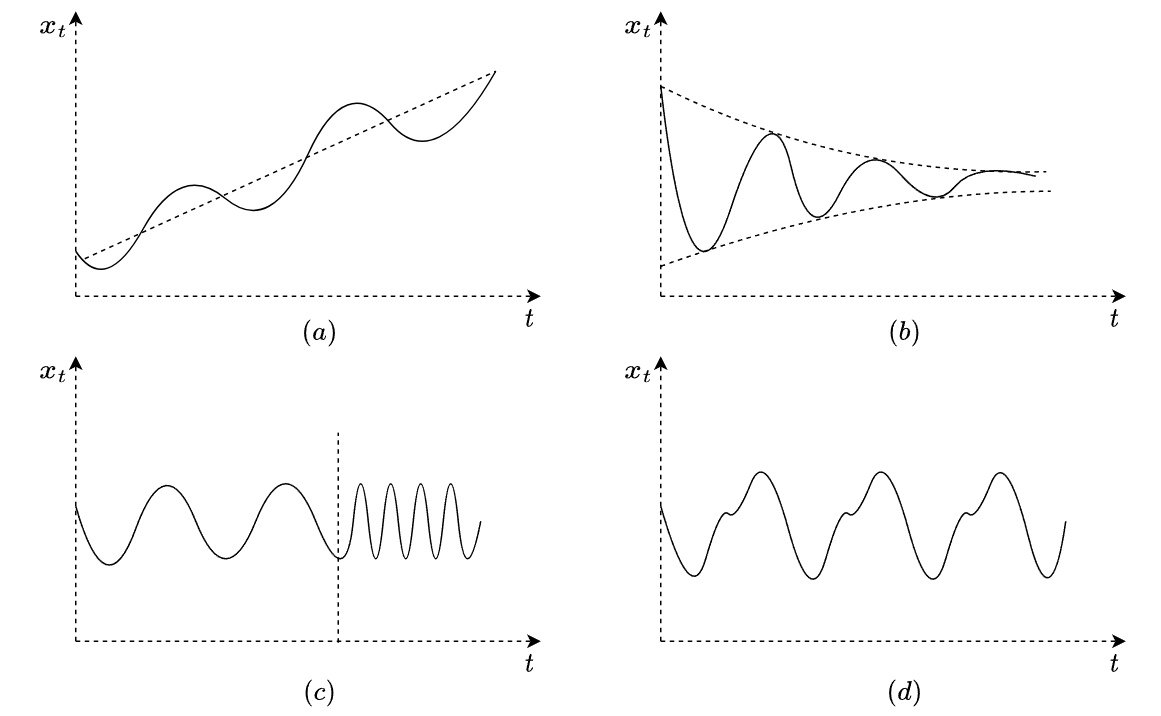
\includegraphics[width=250pt]{../img/09-stationary.png}
        \caption{Figure 9.2:  (a) Non-stationary in mean, (b) non-stationary in variance, (c) time-varying autocovariance (non covariance stationary), (d) stationary time series}
    \end{center}
\end{figure}


If we try to apply linear model to a non stationary variable or a predictor variable is non stationary, the following issues might arise:
\begin{itemize}
    \item When we try to model a variable \(y\) on \(x\), if only \(y\) is non stationary, there is no linear relationship we could describe (\(y\) has a slope but \(x\) does not, so there is no \(y = \beta_0 + \beta_1 x\) that can model the relationship)
    \item If both \(x\) and \(y\) are not stationary, but the degree of growth is different, e.g. \(x\) has a linear growth but \(y\) has an exponential growth, we arrive to the same problem where we are not able to model one variable with another using linear model.
    \item Even if both \(x\) and \(y\) have a linear slope, the relationship between the independent and dependent variable might simply be sporadic correlation (accidental). We could model a growing variable with another, even if there is no relationship. A famous example is a study in 1970 about the increase in margarine consumption and divorce rate in the US.
\end{itemize}

There is also a theoretical reason, which is related to the law of large numbers and the central limit theorem, that we will not explore here.

\subsection{The MA model}

We call a data generating process \textbf{moving average\index{moving average}} if the model has the following form:

\[\operatorname{MA}(k): x_t = \epsilon_t + \theta_1\epsilon_{t-1}  + ... + \theta_k\epsilon_{t-k} \]

where \(\theta_1, ..., \theta_k\) are the weights of the model, and \(\epsilon_{t-1},...,\epsilon_{t-k}\) are i.i.d error terms:

\[\epsilon_{t-1},...,\epsilon_{t-k} \sim i.i.d(0, \sigma^2)\]

The moving average process is stationary and weekly dependent. We can simply find this by applying the model equation to the conditions. Applying to MA(1):

\begin{enumerate}
    \item \(E[x_t] = E[\epsilon_t] + \theta E[\epsilon_{t-1}] = 0\) — constant mean, not a function of time
    \item \(Var(x_t) = Var(\epsilon_t) + \theta^2 Var(\epsilon_{t-1}) = \sigma^2(1 + \theta^2)\) — constant variance, not a function of time
    \item \(\operatorname{Cov}(x_t, x_{t-1}) = \operatorname{Cov}(\epsilon_t + \theta\epsilon_{t-1}, \epsilon_{t-1} + \theta\epsilon_{t-2})\)

We can expand the covariance same as multiplication, but we know error terms are independent, so we only need to consider the recurring error term \(\epsilon_{t-1}\):

\(= \theta \operatorname{Cov}(\epsilon_{t-1}, \epsilon_{t-1}) = \theta Var(\epsilon_{t-1}) = \theta \sigma ^2\)

For a lag \(h\) larger than \(1\)

\(\operatorname{Cov}(x_t, x_{t-h}) = 0\)

Overall it's a function of the lag and not of time
\end{enumerate}

Similarly the correlation will also become \(0\) for lag larger than the lag in the model, making it weakly dependent.

\subsection{The AR model}

The \textbf{auto regressive\index{auto regressive}} or AR model assumes a relationship in the time series between a point in time and a given lag.

\[\operatorname{AR}(k): x_t = \rho_0 + \rho_1 x_{t-1} + ... + \rho_k x_{t-k} + \epsilon\]

Where \(\rho_1, ..., \rho_k\) are the model parameters, \(\epsilon\) is the error term, which is i.i.d with a mean of \(0\) and a variance of \(\sigma^2\):

\[\epsilon \sim i.i.d(0, \sigma^2)\]

The AR model is stationary under certain conditions. If we examine AR(1) and apply it for the conditions of stationary.

\begin{enumerate}
    \item \textbf{Stationary in mean\index{Stationary in mean}}:

\(E[x_t] = \rho_0 + \rho_1 E[x_{t-1}] + E[\epsilon_t]\) \\
\(E[\epsilon_t]\) is simply 0 from the definition. In order for the process to be stationary it must hold that \(E(x_t) = E(x_{t-1})\)  (we will reuse this several times below), substituting these: \\
\(E[x_t] = \rho_0 + \rho_1 E[x_t] \Leftrightarrow\) \\
\[E[x_t] = {\rho_0 \over 1 - \rho_1}\]

For the process to be stationary, we need \(E[x_t]\) to be finite, which means \[\rho_1 \neq 1\] needs to hold, otherwise it's division by 0.

    \item \textbf{Stationary in variance\index{Stationary in variance}}:

\(Var(x_t)=Var(\rho_0+\rho_1x_{t-1}+\epsilon_t)=\rho_1^2V(x_{t-1})+\underbrace{2Cov(x_{t-1},\epsilon_t)}_{=0}+\underbrace{Var(\epsilon_t)}_{\sigma^2}\). In order for the process to be stationary it must hold that \(Var(x_t) = Var(x_{t-1})\): \\
\(Var(x_t)=\rho^2Var(x_t)+\sigma^2 \Leftrightarrow\)

\[Var(x_t)={\sigma^2 \over 1-\rho_1^2}\]

The variance to be positive and finite, we need \\
\(\rho_1^2<1 \Leftrightarrow\)

\[\vert \rho \vert <1\]

    \item \textbf{Covariance stationary\index{Covariance stationary}}:

We can take result of 1., rearrange the elements:

\(E[x_t] = {\rho_0 \over 1 - \rho_1}\) \\
\(\rho_0 = (1 - \rho_1)E[x_t]\) \\
And use this to change the center of the process (original AR(1) formula), removing \(\rho_0\):\\
\(x_t-E(x_t)=\rho_1(x_{t-1}-E(x_t))+\epsilon_t\)

Since it's a recursive function and because \(E(x_t) = E(x_{t-1})\), we can substitute \(x_{t-1}-E(x_t)\) with \(\rho_1(x_{t-2}-E(x_t))+\epsilon_t\):

\(x_t-E(x_t)=\rho_1^2(x_{t-2}-E(x_t))+\rho_1\epsilon_{t-1} + \epsilon_t\)

Repeating \(h\) times:

\(x_t-E(x_t)=\rho_1^k(x_{t-h}-E(x_t))+\sum_{i=0}^{h-1}\rho_1^i\epsilon_{t-i}\)

Shifting by \(h\)  (note that again we don't need to update \(E(x_t)\))

\(x_{t+h}-E(x_t)=\rho_1^k(x_{t}-E(x_t))+\sum_{i=0}^{h-1}\rho_1^i\epsilon_{t+h-i}\)

Calculating covariance with the shifted value (auto covariance), because there is no relationship between \(x\) and the error terms, \(\sum_{i=0}^{h-1}\rho_1^i\epsilon_{t+h-i}\) becomes \(0\):

\begin{flalign*}
& Cov(x_t-E(x_t), x_{t+h}-E(x_t)) \\
& = Cov(x_t-E(x_t), \rho_1^k(x_{t}-E(x_t))) \\
& = \rho_1^k Cov(x_t-E(x_t), x_t-E(x_t)) \\
& = \rho_1^k Var(x_t-E(x_t)) \\
& \text{Redoing tha calculation for stationary in variance (2) but with centered process, gives the same result:} \\
& = \rho_1^k {\sigma^2 \over 1-\rho_1^2} \text{This has the same condition as the stationary in variance:} \vert \rho \vert <1 \\ && \end{flalign*}
\end{enumerate}

\subsection{AR or MA process}

A process that is stationary in mean and variance can be either an AR or an MA process. To diagnose wheater a process is AR or MA, we can look at the autocorrelation, which is:

\(Corr(x_t, x_{t+h}) = {Cov(x_t, x_{t+h}) \over \sqrt{Var(x_t)Var(x_{t+h})}}\)

Because the process is stationary, the variance is constant, so \(Var(x_t) = Var(x_{t+h})\)

\begin{equation}Corr(x_t, x_{t+h}) = {Cov(x_t, x_{t+h}) \over {Var(x_t)}} \tag{9.1}\end{equation}

For an MA(1) process, for \(h = 1\): \({Cov(x_t, x_{t+h}) \over {Var(x_t)}} = {\theta \sigma ^2 \over \sigma ^2(1 + \theta^2)} = {\theta \over 1 + \theta^2}\). For values larger than 1, it was simply 0:

\begin{equation}Corr_{MA}(x_t, x_{t+h}) = \begin{cases}
{\theta \over 1 + \theta^2} & ,\ h = 1 \\
0 & ,\ h > 1
\end{cases}  \tag{9.2}\end{equation}

For an AR(1) process we found that \(Cov(x_t, x_{t+h}) = \rho^k Var(x_t)\), applying to (9.1) we get:

\begin{equation}Corr_{AR}(x_t, x_{t+h}) = \rho^k  \tag{9.3}\end{equation}

While these results look complex they can be very intuitive in identifying if a process is AR or MA. We can plot a graph of our time series, where on the \(X\) axis we have integers \(1, 2, ...\) representing lag, and for each we plot the auto correlation with that lag. This plot is called a \textbf{correlogram\index{correlogram}}.


\begin{figure}[htbp]
    \begin{center}
        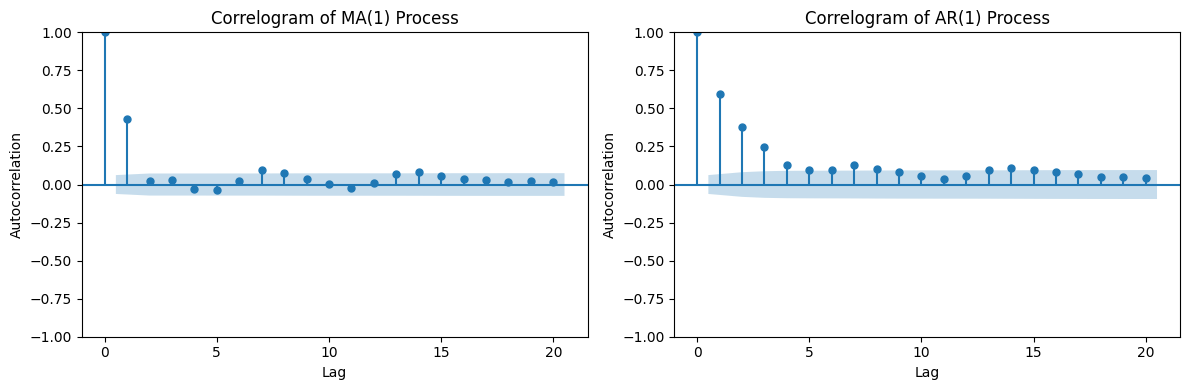
\includegraphics[width=250pt]{../img/09-ma-ar.png}
        \caption{Figure 9.3:  Correlogram of an MA(1) and an AR(1) process.}
    \end{center}
\end{figure}


On \textbf{Figure 9.3\index{Figure 9.3}} we can see the correlogram of an MA(1) and an AR(1) process. All processes have an autocorrelation of 1 with itself with lag 0, so that value does not convey information. The result in (9.2) shows that an MA(1) process will have some value for it's auto correlation at lag \(1\) and \(0\) for lag \(>1\), which is similar to the left side of \textbf{Figure 9.3\index{Figure 9.3}}. The shaded area around the X axis shows statstically insignificant range, correlation values which fall within this range are sampling noise.

An AR(1) model has a non \(0\) auto correlation at lag \(k\), but it:s decaying exponentially as conveyed by (9.3). This same behavior is visible on the right hand side of \textbf{Figure 9.3\index{Figure 9.3}}.

To differenciate an AR(1) processes from AR(2) or higher order, we can use \textbf{partial autocorrelation functions\index{partial autocorrelation functions}}. Partial autocorrelation counts correlation only once, at the lowest lag. The way it does it, it substracts the effect at lag \(k\) from the process and uses this result calculates autocorrelation for the next lag, at \(k+1\) for all \(k=1,2,...\)


\begin{figure}[htbp]
    \begin{center}
        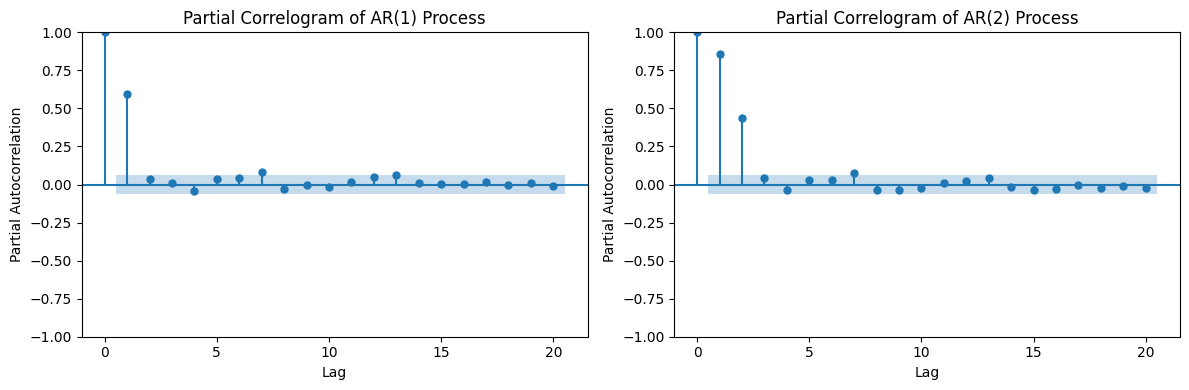
\includegraphics[width=250pt]{../img/09-ar-1-and-2.png}
        \caption{Figure 9.4:  Partial correlogram of an AR(1) and an AR(2) process.}
    \end{center}
\end{figure}


\subsection{Random walk}

An AR(1) process with \(\rho\) of \(1\) is called a \textbf{random walk\index{random walk}}:

\(x_t = x_{t-1} + \epsilon_t\)\\
\(x_t = x_{t-2} + \epsilon_{t-1} + \epsilon_t\)\\
\(x_t = x_0 + \sum_{i=0}^{t-1} \epsilon_{t-i}\)

Since the condition for stationary of variance is violated, it's non stationary time series.

\(Var(x_t) = Var(\sum_{i=0}^{t-1} \epsilon_{t-i}) = \sum_{i=0}^{t-1} Var(\epsilon_{t-i})\)\\
From \(\epsilon_i \sim i.i.d(0, \sigma^2)\), having \(t\) count of noise terms\\
\(Var(x_t) = t \sigma^2\) which is non constant but a function of time.

\subsection{SARIMAX}

SARIMAX is a commonly applied time series analysis technique, it is actually a combination of multiple techniques:

\begin{itemize}
    \item AR: Autoregression
    \item MA: Moving Average
    \item I: Adding differencing to ARMA
    \item S: Seasonality added it ARIMA
    \item X: External parameter added (moving from single variate to multi variate)
\end{itemize}

\section{Non linear modelling of time series data}

Linear models assume some form of linear relationship in time series. If the time series has some non linear relationship and is not purely a random walk or white noise we can try to fit a non linear model.

A number of machine learning techniques we discussed so far as well as new techniques developed for sequential data can be fit to model time series. If a model is successfully fit on a time series, it can be used for forecasting unseen/future values.

\subsection{Neural networks in time series}

One simple approach is to train a deep neural network with \(k\) inputs capturing the relationship among \(k\) consecutive samples in the time series. A challenge is that we might not know \(k\) but also that \(k\) might differ for a test dataset or even among training sets.

To support a variable number of inputs, which form a sequence, where previous values influence future or upcoming values, an extension of neural network has been developed called \textbf{recurrent neural network\index{recurrent neural network}} or \textbf{RNN\index{RNN}}. The difference between an RNN and a multilayer network is that these networks have \textbf{feedback loops\index{feedback loops}}.

Just as with multilayer network we define an input at position or time \(t\) as \(X_t\) which can be single value (scalar) or multiple values (vector). Assuming the more complex case, where we have multiple inputs at each moment \(t\), \(X_t\) would be a vector of dimension \(d_x\).

A common structure for RNN has a single hidden layer with a non linear activation function, noted with \(f_h\), also used for the feedback loop, and an output activation, noted with \(f_Y\). These two activation functions might be of different type, for example the hidden layer activation \(f_h\) might be a tanh function while the output activation \(f_Y\) might be a softmax function.

An RNN, similar to multilayer networks, has weights and biases. RNNs introduce one more set of weights, noted here with the matrix \(W_{hh}\) for the feedback loop, the output of a network would become an input as well. The hidden layer can have one or more neurons, we can note this number with \(d_h\). \(W_{hh}\), representing the weights between all neurons in the hidden layer to all other neurons, would be a square matrix with dimension \(d_h \times d_h\).

Similar to multi layer networks, we have weights associated with inputs which we can represent as a matrix \(W_{Xh}\) of dimension \(d_x \times d_h\), mapping inputs to hidden layer neurons. Using the activation for the hidden layer \(A_h\), the recurrent relationship can be written as:

\[h_t = A_h(W_{Xh} X_t + W_{hh} h_{t-1} + b_h)\]

Where \(b_h\) is the bias term for the hidden layer.The output of an RNN for time step \(t\) can be computed as:

\[Y_t = A_Y(W_{hY} h_t + b_Y)\]

The weight matrix \(W_{hY}\) that transforms the hidden state to the output space has the shape of \(d_h \times d_Y\), where \(d_Y\) is the dimensionality of the output. \(b_Y\) is the bias term for the output.

To combine the two formula into a single, more continuous formula, would be:
\[Y_t = A_Y(W_{hY} \times A_h(W_{xh} X_t + W_{hh} h_{t-1} + b_h) + b_o)\]


\begin{figure}[htbp]
    \begin{center}
        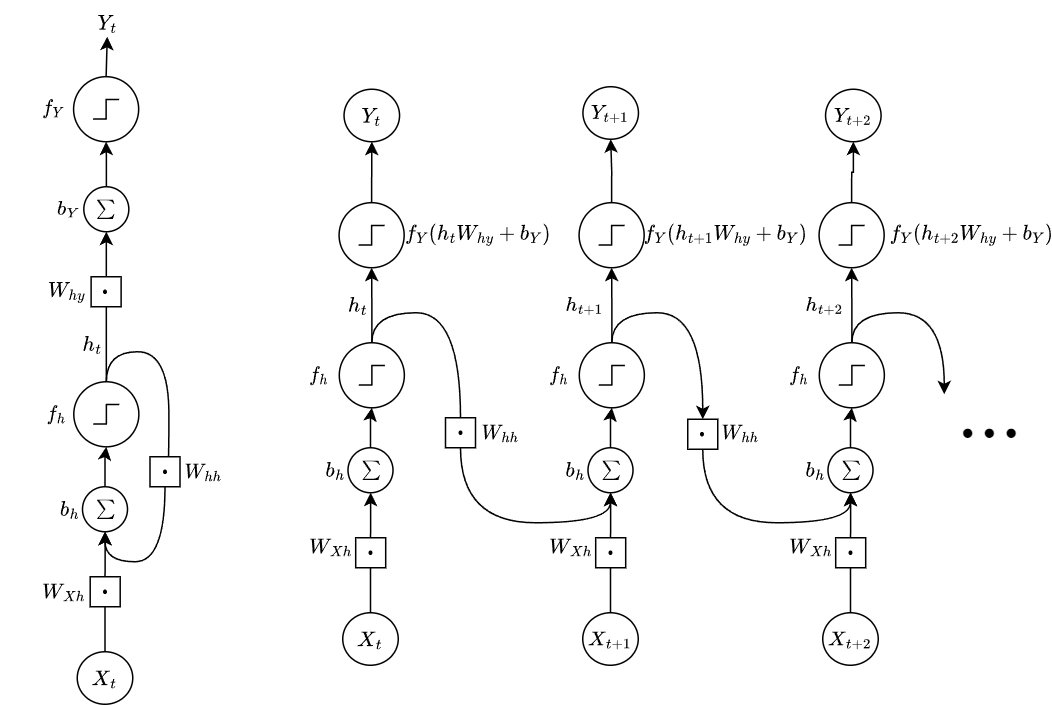
\includegraphics[width=300pt]{../img/09-rnn.png}
        \caption{Figure 9.5:  Left: structure of an RNN, right: unrolling of the network}
    \end{center}
\end{figure}


\textbf{Figure 9.5\index{Figure 9.5}} shows the RNN visually. On the left side we can see the feedback loop. This network can be unrolled by making copies of the network, in which case the feedback loop would become input for the next copy. This process is called unrolling and has been used by state of the art network at the time of writing this material. The right side of the diagram shows the unrolled version of the network.

\textbf{Modelling an AR(k) model with RNN\index{Modelling an AR(k) model with RNN}}

While it is not efficient to use RNN for an AR(k) process, it is a useful way to understand how RNN works and extends the AR process. Applying RNN would probably introduce unnecessary variance and overfit the model. But if we were to model an AR(k) process defined as \(x_t = \rho_0 + \rho_1 x_{t-1} + ... + \rho_k x_{t-k} + \epsilon\) the RNN would have the following properties:

\begin{itemize}
    \item Input would be a scalar, the value of the time series at time \(t-k\) leading up to \(t-1\). The output would also be a scalar, the prediction, or current value: \(x_t\).
    \item The hidden layer would need to have \(k\) activation functions, where both the hidden layer and output activation functions would be linear function: \(f_h(x) = f_Y(x) = x\) for all values of \(x\).
    \item The weights on the output layer would be the identity matrix \(I\), with each diagonal value of \(1\) and off diagonal element of \(0\)
    \item While multiple set of weights on the hidden layer could model an AR(k) process, a very straightforward option would be a diagonal matrix, where each diagonal element would be a coefficient of the AR(k) process: \(\rho_1 ... \rho_k\). The bias term would be equal to \(\rho_0\)
\end{itemize}

Such a recurrent network would be equivalent with the AR(k) process. If we were to train an actual RNN using samples from an AR(k), we would probably end up with a different but equivalent definition of weights, resulting from the random initialization of the network.

Notice the points that we simplified and if we are to utilize, can capture more complex relationships in the time series:

\begin{itemize}
    \item When we modelled an AR(k) process, we used only a small potion of the available weights. We can leverage off diagonal elements in the hidden layer as well as the weights in the output layer to create a more complex model.
    \item Non linear activation functions can capture non linear relationship between the points in time as well as in the output mapping. Interactions between the inputs can also be approximated
    \item Using identity matrix for weights as well as linear activation, we effectively removed the output layer.
    \item An RNN can handle multiple inputs and outputs.
\end{itemize}

\textbf{Considerations of RNN\index{Considerations of RNN}}

An RNN, even when we consider the unrolled version, still uses the same weights for each copy. To scale an RNN, the simplest way is to increase the neurons in the hidden layer. Another option is to stack multiple RNNs, the output of the first RNN would be the input of the second RNN and so forth.

RNNs provide a useful way to think about neural networks but in practice it's rarely used in it's simplest form. The biggest challenge of RNN is it's difficulty of training. In practice, the more we unroll an RNN network, will behave like a really deep neural network. All the difficulties of training deep neural networks arise in a magnified manners.

More specifically the issue is that weight training is unstable, leading to \textbf{vanishing\index{vanishing}} or \textbf{exploding gradients\index{exploding gradients}} problems. Considering a single weight in the hidden layer, noted with \(w\) and the input \(x\), a network unrolled \(n\) times, the loss function will contain the output of the network compared with the training data set, which in turn will have in it's formula the expression \(x w^n\). If \(n\) is large, e.g. 100, which can happen easily for time series inputs like price changes across time, the expression \(x w^n\) can become close to \(0\) if \(w < 1\) or very large for \(w > 1\). In the backpropagation process we calculate the gradient of the loss function, which will have similar behavior, resulting in the problem of vanishing gradient (\(n \gg 1, w < 1 \rightarrow w^n \approx 0\)) or exploding gradient (\(n \gg 1, w > 1 \rightarrow w^n \approx \infty\)).

To resolve the vanishing/exploding gradient issue, further variations of RNN has been proposed. Sepp Hochreiter and Jürgen Schmidhuber in their paper called "Long Short-Term Memory" defined \textbf{Long Short Term Memory\index{Long Short Term Memory}} networks, \textbf{LSTM\index{LSTM}} in brief. They applied gating mechanism and two tracks to maintain a long term memory and a short term memory, while keeping the network easier to train. In more recent years, the attention and transformer architecture has seen great results, outperforming LSTM in both ease of training and ability to maintain memory. Transformer architecture has seen great results being applied to time series, also allowing for multivariate time series forecasting, using other features available in the data. We will explore transformer architecture in the context of natural language processing and large language models, but the same architecture can be used for time series as well.

\subsection{Tree models in time series modelling}



\subsection{Trend and seasonality modelling - Facebook Prophet}



\chapter{Natural language processing}

\textbf{Natural language processing\index{Natural language processing}} or \textbf{NLP\index{NLP}} for short the field of AI concerned with working with natural languages like English (as opposed to programming language like Python) is one of the fastest growing fields of AI in recent years.

\section{Common NLP terms and statistics}

\textbf{Tokenization\index{Tokenization}} breaks a text into tokens, in most cases words. In English punctuation and white spaces can be used. Sentence ending punctuation should be unified to a token signifying sentence boundary. In some languages like Chinese, where spaces are not used as word separator, dictionaries are required for tokenization. Some special types of tokenizers:
\begin{itemize}
    \item \textbf{Contraction\index{Contraction}} is a form of tokenization mainly for grammatical structures like `wasn't`, splitting into `was` and `n't` or when possible to it's full form of `was` and `not`, so each new token has a meaning on their own. THis helps to reduce the number of tokens and also to covey more meaning to the model.
    \item \textbf{Casual tokenization\index{Casual tokenization}} when we want to work with social media content, it's often required to remove handlers (e.g. `@username`), emoticons, character repetitions (e.g `loool` can be normalized to `lol`)
\end{itemize}

\textbf{Normalization\index{Normalization}} can be used to unify tokens with same meaning. Search engines might apply stronger normalization, to increase \textbf{recall\index{recall}} metric as the number of matches against (possibly much bigger reduction in) \textbf{precision\index{precision}}. For NLP pipelines normalization might reduce too much context so might be reduced or skipped entirely. Common normalization techniques are:
\begin{itemize}
    \item \textbf{Case folding\index{Case folding}}: unifies upper and lower case, which might be applied to sentence starting words only but skipped for proper nouns, like names.
    \item \textbf{Ascii folding\index{Ascii folding}}: unifies special characters to more common forms, e.g in languages which use accents like `á` can be normalized to English letters `a`.
    \item \textbf{Lemmatization\index{Lemmatization}} using part of speech, can convert words entirely to other, more common words with same meaning e.g `better` as an adjective might be normalized to `good`
    \item \textbf{Stemming\index{Stemming}} normalizes words to their stem, removing grammatical structures like plural form. Usually applied after lemmatization, more simple to implement compared to lemmatization but also reduces more meaning. This might be achieved with a complex language specific rule set, e.g `spelling` simply remove `ing`, `handling` remove `ing` but restore the missing `e`, the `ing` in `ping` is not a grammar form so cannot be removed. Another option is to use statistical tools.
\end{itemize}

\textbf{Part of speech (PoS) tagging\index{Part of speech (PoS) tagging}}

\textbf{Named entity recognition\index{Named entity recognition}}

\textbf{Syntactic parsing\index{Syntactic parsing}}



\subsection{TF-IDF}

A common statistic or scoring used with natural language documents is the \textbf{term frequency, inverse document frequency\index{term frequency, inverse document frequency}} or TF-IDF. The primary use case of TF/IDF is document retrieval based on a search term. Given a set of documents, we can calculate TF/IDF score for each document \(d\) in our set for the search term \(t\). TF-IDF can be broken down as a relationship between two other statistics, TF and IDF:

\[\operatorname{TF-IDF} = \operatorname{TF} \cdot \operatorname{IDF}\]

The TF term for a document (\(d\)) given the term (\(t\)) is defines how many times a word appears in a document as an importance between the document and the term.

\[\operatorname{TF}(t,d) = {count(t\ in\ d) \over {count(*\ in\ d)}}\]

According to \textbf{Zip'f law\index{Zip'f law}} most languages follow a pattern. If we count the term frequencies and rank them in decreasing order, the frequency of any word is inversely proportional to it's rank. Given a large enough corpus in English, the first term would be `the` occurring 2 times as `of` at rank 2, 3 times as `to` at rank 3, 4 times as `a` at rank 4, etc. Other languages will follow a similar pattern.

The inverse document frequency defines how common the term is in terms of the corpus. Words which appear frequently in all documents will get a higher IDF score compared to words that are unique to some documents. For large scale corpus the IDF term can explode, so commonly the natural log is used to scale:

\[\operatorname{IDF}(t) = ln\bigg({N \over count(t\ in\ D)}\bigg)\]

where \(D\) is the set of all documents and N is the total number of documents. The choice for natural log instead of other base is mainly for consistency. If the term \(t\) does not exist in \(D\), a division by \(0\) can occur. A common solution is to add \(+1\) to the denominator:

\[\operatorname{IDF}(t) = ln\bigg({N \over count(t\ in\ D)  + 1}\bigg)\]

A similar result would be provided if we apply a technique called \textbf{Laplace smoothing\index{Laplace smoothing}}.

TF-IDF is commonly used as a document retrieval in document stores. A commonly used document store is ElasticSearch which uses BM25, an extended version of TF/IDF to rank documents given a list of search terms or tokens. For each token and each document a TF/IDF score can be computed. The TF-IDF scores resulting in the case of multiple tokens can  be combined with a simple summation or weighted summation. The resulting combined TF-IDF scores for each document determines the most relevant documents for the search terms.

\section{Primitive language models}

Primitive language models, while less used on their own, and rather as part of larger system, still provide useful basis for us to explore.

\subsection{Bag of words}

The \textbf{bag of words\index{bag of words}} (BoW) model is a common representation used in NLP. We can use it to represent a sentence, usually part of a set of sentences or corpus, as a vector. The steps are as follows:

\begin{enumerate}
    \item Assign all terms from our corpus to an index from \(1\) to \(|V|\), where \(|V|\) is the total number of unique terms in our corpus (\(V\) is the set of terms).
    \item Construct a vector of size \(|V|\)
    \item For each element at index \(i\) assign\\
a.) \(1\) if the word \(i\) is in the sentence, \(0\) otherwise - called binary BoW\\
b.) Number of occurrences of the word \(i\) in the sentence, also called term frequency or TF\\
c.) TF/IDF score of the word \(i\), TF would capture how important the term is for the sentence, IDF would measure how important the word is considering the entire corpus\\
d.) normalized frequencies - number of times the word \(i\) occurs in the sentence divided by the total number of words in the sentence. This normalization ensures that longer documents do not have an inherent advantage over shorter ones.
\end{enumerate}

BoW vectors are very sparse so not too practical, but they can already be used with vector arithmetics. The dot product of two binary BoWs would give a similarity measure between sentences in terms of how many words repeat across the two sentence.

In most cases we want to measure if documents have similar words in similar counts as a measure of distance. In the \(|V|\) dimensional space where every word is a dimension, the best measure for this is the angle between two BoW vectors. We can quantify the distance as an angle with \textbf{cosine similarity\index{cosine similarity}}:

\[cos\ \Theta = {A \cdot B \over |A| |B|} = {\sum_{i=1}^{|V|} a_ib_i \over \sqrt {\sum_{i=1}^{|V|} a_i^2} \sqrt {\sum_{i=1}^{|V|} b_i^2}}\]

where \(A\) and \(B\) are two BoW vectors, \(A \cdot B\) is the dot product, \(|A|\) and \(|B|\) are the L2 norms of the vectors. The above expression might be more familiar in the form of \(A \cdot B = |A| |B|\ cos\ \Theta\). Cosine similarity ranges between \(-1\) and \(1\), where 1 means that the two vectors point in the same direction, but their magnitude might be different. Since term frequencies cannot be negative, for BoWs the minimum cosine similarity would be 0, which happens for perpendicular vectors, meaning that no common word is being used in two sentences.

\subsection{Naive Bayes}

\textbf{Naive Bayes\index{Naive Bayes}} can be used to classify a text to some category, given a training data set. in the context of NLP it's used a a non-parametric estimator. From Chapter 5, the Naive Bayes classifier is as follows:

\begin{equation}{\displaystyle C^{\text{Bayes}}(x)={\underset {k}{\operatorname {argmax} }} P (Y=k)\prod _{j} P(X_j = x_j|Y=k)}\tag{10.1}\end{equation}

In the context of NLP the class is usually a category. This model is also used for sentiment analysis, where each sentiment is treated is a category. For example given a list of product reviews (e.g app store reviews) with both a text and a five star review, a Naive Bayes model can be constructed to also evaluate tweets about the product without explicit ratings.

Given a sentence \(x\) we want to classify it to a category \(k\) using Naive Bayes: \(\displaystyle C^{\text{Bayes}}(x)\). Every word in the sentence acts as a predictor \(x_i\).  Naive Bayes assumes that the probability of a combinations of words (or the lack of words) defining the class of sentence is same as the probability for each word separately doing the same. In most cases, this is not true, e.g \textit{g}oal\textit{ }will have a different meaning if it's combined with the word \textit{c}areer\textit{ }and different meaning if occurs together with \textit{s}occer\textit{.}

To apply Naive Bayes a training dataset is needed, also called \textbf{corpus\index{corpus}} in the context of NLP. The term \(P(Y=k)\) called the prior, can be calculated as the ratio of training sentences of class \(k\), noted with \(n_{\operatorname{x} \rightarrow k}\), divided by number of total training samples \(N\)

\[P(Y = k) = {n_{\operatorname{x} \rightarrow k} \over N}\]

For each word in the training dataset, we can create a distribution of how likely each word predicts a category as the ratio between the number of occurrences of the word in sentences of class \(k\), noted as \(n_{\operatorname{x_i} \rightarrow k}\), divided by the total number of words in sentences of class \(k\), noted with \(n_{\operatorname{x_* \rightarrow k}}\):

\[P(X = x_i | Y = k) = {n_{\operatorname{x_i} \rightarrow k} \over n_{\operatorname{x_* \rightarrow k}}}\]

This probability is also referred to as likelihood.

When we get a new sentence we can predict the category by plugging in the prior and likelihood for each word calculated using the training data, into 10.1.

If the test sentence has a word that does not appear in a category in the training set, the likelihood term will be \(0\) and the probability for that category will also become \(0\) irrespective of the likelihood of other words in the sentence. To counter this we can change the likelihood as

\[P(X = x_i | Y = k) = {n_{\operatorname{x_i} \rightarrow k} + q \over n_{\operatorname{x_* \rightarrow k}} + Nq}\]

where \(q\) is a constant, usually with a value of 1. This will result as minimum likelihood of \(1 \over N\).

The BoW can be used as an input to "train" the Naive Bayes model. We can create a single BoW for each category, where each index \(i\) would capture how many sentences contains that word.

\subsection{N-gram model}

In the context of index creation for document retrieval we usually talk about n-grams in the context of characters. In the string `abc` the possible 2-grams are `ab` and `bc`. Edge n-grams from left side are `a`, `ab` and `abc`.

In the context of NLP, the n-gram model is defined in context of words. We are trying to capture groups of words that occur together in a specific order. This information was last in BoW and Naive Bayes models.

Too infrequent (lyrical word combination) and too frequent (e.g. `at the`) n-grams are not useful for modelling and might contribute to overfitting. The simplest way to get the useful n-grams is to apply \textbf{rare token\index{rare token}} (exclude too rare n-gramns) and \textbf{stop word\index{stop word}} filters (exclude too common n-gramns). Stop word filters should be applied to n-grams and not the stop words themselves, since n-grams can capture relationship between stop words and other words (4 grams might be needed for this).

N-gram model is a simple probabilistic model, where we try to predict the next word, given \(n-1\) previous words. For a given n-gram sequence of words \(w_1, w_2, \ldots, w_n\), the probability of the n-gram can be defined as:

\[P(w_n | w_1, w_2, \ldots, w_{n-1})\]

This probability is typically estimated from a corpus using Maximum Likelihood Estimation (MLE):

\[P_{MLE}(w_n | w_1, w_2, \ldots, w_{n-1}) = \frac{\text{Count}(w_1, w_2, \ldots, w_n)}{\text{Count}(w_1, w_2, \ldots, w_{n-1})}\]

Where:
\begin{itemize}
    \item \(\text{Count}(w_1, w_2, \ldots, w_n)\) is the number of occurrences of the n-gram sequence \(w_1, w_2, \ldots, w_n\) in the corpus.
    \item \(\text{Count}(w_1, w_2, \ldots, w_{n-1})\) is the number of occurrences of the \(n-\) gram sequence \(w_1, w_2, \ldots, w_{n-1}\) in the corpus.
\end{itemize}

One of the main challenges with n-gram models is dealing with zero counts (i.e., unseen n-grams in the training data but may appear in the test data). To address this, various smoothing techniques are use, for example Laplace Smoothing:

\[P_{\text{Laplace}}(w_n | w_1, w_2, \ldots, w_{n-1}) = \frac{\text{Count}(w_1, w_2, \ldots, w_n) + k}{\text{Count}(w_1, w_2, \ldots, w_{n-1}) + k V}\]

Where:
\begin{itemize}
    \item \(V\) is the vocabulary size.
    \item \(k\) is a small positive number (often set to 1).
\end{itemize}

N-gram models despite their simplicity have some important use cases. We can perform tasks like:

\begin{itemize}
    \item Sentence Probability: Evaluate the likelihood of a given sentence or sequence of words.
    \item Text Generation: Predict the next word in a sequence, which can be useful for autocompletion or generating text. Similar how Google Search is able to predict next words typed in the search bar.
\end{itemize}

\subsection{Latent Semantic Analysis (LSA)}

\subsection{Word2Vec}

A seminal development in natural language processing occurred in 2013 when Tomas Mikolov and his colleagues at Google released a paper titled "Efficient Estimation of Word Representations in Vector Space", which introduced the concept now popularly known as Word2Vec.

Word2Vec models are neural networks that try to learn a vector representation of words, also called \textbf{embeddings\index{embeddings}}. Embeddings are dense vectors (dense is the opposite of sparse, dense means there are few non zero elements). Words with similar meanings should be close to each other in the high dimensional space represented by the vector. As we seen in the case of bag of words, distance can be measured using cosine similarity. To train these models, a text corpus is used similar to other models discussed, instead of a special annotated data set.

The input of the model is using \textbf{one hot encoding\index{one hot encoding}} of words in the vocabulary. One hot encoding is a high dimensional highly sparse representation. Each word is represented by a vector, with the size of the vocabulary \(V\). Each word is assigned a unique index \(w_1 \rightarrow 1, w_2 \rightarrow 2, \ldots, w_{V}  \rightarrow V\). The one hot encoding of a word is a vector of \(0\) s, and a single, at the assigned index having value of \(1\):

\(w_1 \rightarrow \{1, 0, \ldots, 0\}, \\
w_2 \rightarrow \{0, 1, \ldots, 0\}, \\
\vdots \\
w_V \rightarrow \{0, 0, \ldots, 1\}\)

In a corpus using English language there are about 60,000 words, so the input vector will have this size. Word2Vec transforms these vectors to a lower dimension, usually around 200, but ranging from 50 to more than 300 depending on the corpus size, and available compute resource. Word2Vec can be thought of as a dimensionality reduction method or an encoder.

Prior to Word2Vec, research was done on using neural networks in a similar fashion using feed forward as well as recurrent neural networks, using a hidden layer, but the non linear activation function seemed too heavy on computation given the large size of hidden layers and inputs. Word2Vec uses no activation in the hidden layer, only in the output layer.

The model is trained using the context of a word as it appears in the corpus used. The context is defined by surrounding words, words that appear before or next to the target word. Depending on how neighboring words are used, two types of networks are defined:

\begin{itemize}
    \item In the \textbf{Skip-Gram\index{Skip-Gram}} model the target word is used to predict its context (surrounding words).
    \item In the \textbf{continuous Bag-of-Words (CBOW)\index{continuous Bag-of-Words (CBOW)}} model, the process is reversed: the context (surrounding words) is used to predict the target word.
\end{itemize}


\begin{figure}[htbp]
    \begin{center}
        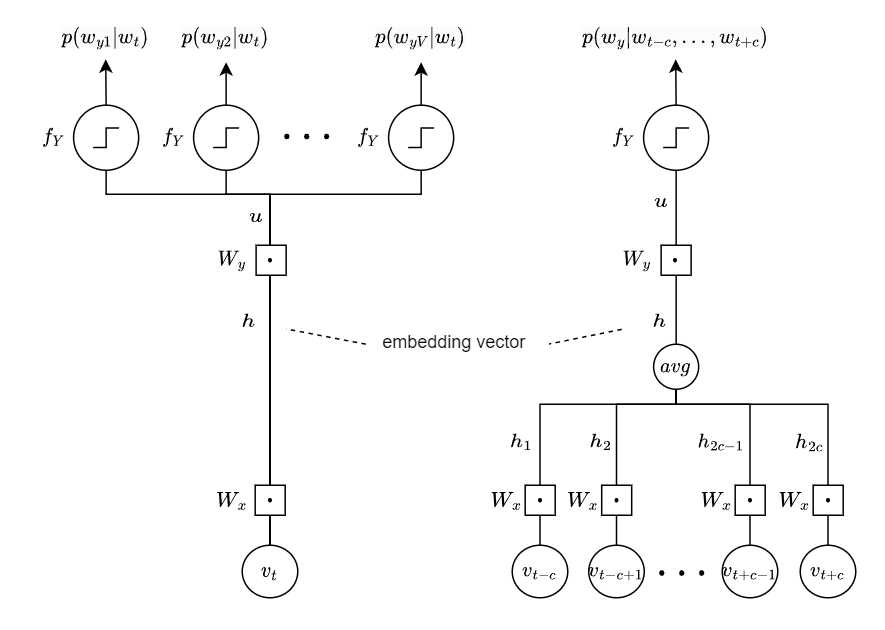
\includegraphics[width=300pt]{../img/10-word2vec.png}
        \caption{Figure 10.1: <i>Architecture of Word2vec, left it skip-gram, right is CBOW model</i>}
    \end{center}
\end{figure}


To describe the model, we define words in the vocabulary as \(w\). \(w_t\) is the target word, \(t\) representing position in the text (moment, time). We note with \(v\) the one hot encoding of the word \(w\).

We note the context window of a word with \(c\) in either direction, usually chosen as \(c = 5\), so the model will consider 5 words before and 5 words after the target word. As seen on Figure 10.1, skip-gram tries to estimate the context given the word \(w_t\) (and it's one hot encoding \(v_t\)), while CBOW uses the context as input to estimate the probability of the target word. Also notice that the network does not have a bias term.

The output activation function \(f_Y\) used to estimate the probability distribution is the softmax function. The softmax function is often used to estimate probability distributions, because its outputs are values between \(0\) and \(1\), and all output sums to 1, so follows some properties of a probability distributions. We need to note that it's not the actual probability distribution, only an estimate. If we change the initial weights in the network, it will change the distribution. Another reason why it is an estimate is because the actual probability might be an infinitely complex function, while here we have a limited number of weights and not all contextual information is used to find the correct probability.

\textbf{Skip gram model\index{Skip gram model}}

Starting with the skip-gram model, the input is a single word with one hot encoding \(v_t\) with the size of the vocabulary \(V\).

The hidden layer \(h\) is a vector of size \(N\) and is given by a matrix-vector product between the input weight matrix \(W_x\) of size \(N \times V\) with the input \(v_t\).

\[h = W_x v_t\]

The output \(u\) layer has a second set of weights, represented by the matrix \(W_y\) of size \(V \times N\) (dimensions are flipped compared to \(W_x\)), transforming the hidden dimension of N back to the one hot encoding dimension of \(V\) (number of words in the vocabulary).

\[u = W_y h = W_y W_x v_t\]

We finally estimate for \(2c\) words as being context words of \(w_t\).

\[p(w_k|w_t) = f(u_k) = {\operatorname{exp}(u_k) \over \sum_{i-1} ^V \operatorname{exp}(u_i)}\]

The network will have \(2c\) vectors as output. \(k\) goes from \(t-c\) to \(t+c\) but skips the value of \(t\) because that is the target word \(w_t\), used as input. \(u_i\) is the \(i\) th element of \(u\). The expression \(\operatorname{exp(x)}\) is same as \(e^x\) used here to make formula more easy to read.

\textbf{CBOW model\index{CBOW model}}

CBOW tries to estimate the target word given it's context. A window is chosen as context. CBOW has input of \(2c\) vectors, where \(c\) is the context window size in either direction. Similar to skip-gram, we apply the input weight matrix, but this would result in \(2c\) vectors \(h_i, i = 1 \ldots 2c\). To get the hidden layer \(h\) the model averages all the \(h_i\) vectors. This is shown visually on the right side of Figure 10.1.

\[h = \frac{1}{2c} \sum_{i = 1}^{2c} h_i = \frac{1}{2c} \sum_{i = -c \ldots c ,\  i \ne 0} W_x v_c\]

In the CBOW model we calculate the target word from the context so we have a single output. The output score is calculated in similar way to skip gram

\[u = W_y h = \frac{1}{2c} \sum_{i = -c \ldots c ,\  i \ne 0} W_y W_x v_c\]

The probability distribution estimate of a word \(w_t\) being the target word for context \(w_{t-c}, \ldots, w_{t-1}, w_{t+1}, \ldots, w_{t+c}\) noted with \(C_t\) is given by:
\[p(w_t|C_t) = \frac{\exp(u_{t})}{\sum_{i=1}^{V} \exp(u_i)} \]

While the softmax output looks similar, please note that skip-gram had \(2c\) outputs while CBOW has \(2c\) input and a single output.

\textbf{Fitting Word2Vec\index{Fitting Word2Vec}}

To fit the model the negative log likelyhood loss function can be used. Since skip gram has \(2c\) outputs representing the context of the word, we need to average the likelyhoods.

Given our corpus represented as a word sequence \(w_1, \ldots, w_T\) the loss function is the average likelyhood for each word \(1 \ldots T\), and within each word for each context:

\[\theta_{\operatorname{skip\ gram}} = -\sum_{t=1}^{T} \sum_{-c \leq j \leq c, j \neq 0} \log p(w_{t+j}|w_t)\]

For CBOW the model has single output so the objective function does not need to average the context (it has been done during calculation of the hidden layer \(h\))

\[\theta_{\operatorname{CBOW}} = -\sum_{t=1}^{T} \log p(w_t,C_t)\]

In practice, Word2Vec is quite difficult to train, given a large corpus, thus to optimize training, further techniques like hierarchical softmax or negative sampling were proposed. Since here we want to describe Word2Vec as a way to explain transformers, and these optimizations are not used by transformers we will omit the detailed exploration of these techniques.

Once the model is fit, the hidden layer \(h\) is the word embeddings extracted and used. Word embedding vectors can be used as a simple arithmetic with the famous example of:

\[h(\operatorname{"Man"}) - h(\operatorname{"King"}) + h(\operatorname{"Woman"}) \approx h(\operatorname{"Queen"})\]

We used the operator \(\approx\), because vector the operations might not give the exact relationship, if we search for the closest vector using cosine similarity to find the result, the \(h(\operatorname{"Queen"})\) can be found. In practice output embeddings can be used directly, like finding similar words (e.g information retrieval), or as input to another model, like a sentiment analysis classifier or sequence to sequence models used for translation.

The context window used by Word2Vec, more so in the case of CBOW carries some conceptual similarity to the convolution layer in image processing networks, like having a local reception area, a small square of an image vs a number of consecutive words in a text, though the processing and output is used differently.

\section{Large Language Models}

Based on research on RNN networks, LSTMs and other techniques discovered at the time, a breaktrough in natural language processing happened in 2017 when Google researchers led by Ashish Vaswani published the paper "Attention Is All You Need" starting the advent of more efficient and easier to train large language models, most notably BERT and GPT. GPT models became famous in 2022 trough the service called ChatGPT, which used GPT model 3.5. The chat service, despite it's simplistic interface, has seen a record high user base growth.



\chapter{Image processing}


\chapter{Searching and recommenders}


\chapter{Reinforcement learning}


\chapter{Unsupervised learning}


\chapter{Bayesian networks and causality}


\chapter{Machine learning project process and system design}


\chapter{Appendix I - mathematical notations and concepts}

\section{Argmin and argmax}

\(\operatorname{argmin}_x f(x)\) is the value of \(x\) for which \(f(x)\) attains its minimum.

Similarly, \(\operatorname{argmax}_x f(x)\) is the value of \(x\) for which \(f(x)\) attains its maximum. Minimization can be transformed to maximization problem as

\[\operatorname{argmax}_x f(x) = \operatorname{argmin}_x -f(x)\]

The difference between \(\min f(x)\) and \(\operatorname{argmin}_x f(x)\) is that the first one is the minimum value of the function \(f(x)\), \(\operatorname{argmin}_x\) is a value of \(x\), where \(f(x)\) is minimum.


\chapter{Appendix II - Linear algebra}

In this appendix we describe linear algebra, not from axioms, rather from intuitive, geometric understanding of vectors and matrices.

Linear algebra is the study of vector spaces. For machine learning the most important vector space, is the \textbf{normed vector space\index{normed vector space}}, which defines a norm, noted with \(\|\cdot\|\), that simply means length.

The building blocks of vector spaces are real or integer numbers, called \textbf{scalars\index{scalars}}, vectors and matrices.

We will build the intuition of vectors and matrices using examples in two dimensions, but all concepts equally apply for higher dimensions as well, visualizing concepts above two or three dimensions are extremely challenging and not too helpful.

\section{Vectors}

There are many interpretations of vectors depending on the field of science. For vector spaces the simplest interpretation of an \(n\) dimensional vector, is an \(n\) dimensional arrow, having a tail always at the origin, and pointing to a coordinate defined by the \(n\) scalars.

Vectors are usually noted with an arrow above a lowercase letter (e.g \(\vec{v}\)) or with an uppercase letter (e.g \(V\)). A vector can also be represented as an ordered list of it's \(n\) components, usually written as a column:

\[V = \begin{pmatrix} v_1 \\ v_2 \\ \vdots \\ v_n \end{pmatrix}\]

\(n\) is also called the dimensions of the vector. The set of all \(n\) dimensional vectors of real numbers is noted with \(\mathbb{R}^n\).

A special vector, of size \(0\), starting and ending in the origin has all elements as \(0\).

\[O = \begin{pmatrix} 0 \\ 0 \\ \vdots \\ 0 \end{pmatrix}\]

Figure II.1 shows an example of a two dimensional vector \(\begin{pmatrix} a \\ b\end{pmatrix}\), where \(a, b \in \mathbb{R}\). An intuition about vectors is that they represent movement, similar to the interpretation in physics.


\begin{figure}[htbp]
    \begin{center}
        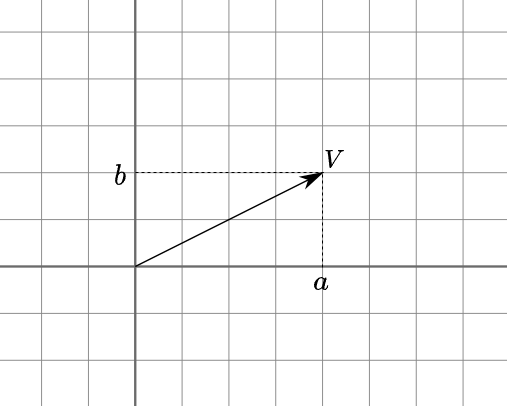
\includegraphics[width=150pt]{../img/ii-vector.png}
        \caption{Figure II.1: A two dimensional vector, having tail at origin (0, 0) and pointing to (a, b), where a and b are real numbers. Normed vector spaces define length, noted with a grayed grid as the unit steps on the space}
    \end{center}
\end{figure}


Addition of two arrays is defined as pairwise addition of it's elements

\[U+V = \begin{pmatrix} u_1 \\ u_2 \\ \vdots \\ u_n \end{pmatrix} + \begin{pmatrix} v_1 \\ v_2 \\ \vdots \\ v_n \end{pmatrix} = \begin{pmatrix} u_1 + v_1 \\ u_2 + v_2 \\ \vdots \\ u_n + v_n \end{pmatrix}\]

In figure Figure II.2 we illustrate the geometric interpretation of the vector addition. If we continue our interpretation of vectors as movement, the sum of the two movement can be considered as continuing the second movement where the first ended. To represent this visually, we can move the tail of one vector to the arrow head of the other (this is the only exception when we move a vector's tail from origin). The resulting point of the second vector tip is the sum of the two vectors.


\begin{figure}[htbp]
    \begin{center}
        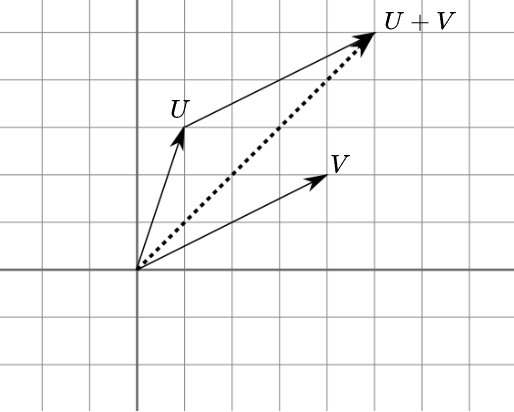
\includegraphics[width=150pt]{../img/ii-addition.png}
        \caption{Figure II.2: Addition of two vectors U and V}
    \end{center}
\end{figure}


Multiplication of a vector with a scalar is defined as multiplying each element of the vector with the scalar:

\[c \cdot V = c \cdot \begin{pmatrix} v_1 \\ v_2 \\ \vdots \\ v_n \end{pmatrix} = \begin{pmatrix} c \cdot v_1 \\ c \cdot v_2 \\ \vdots \\ c \cdot  v_n \end{pmatrix}\]

This will change the scale (or norm) of the vector but not the direction of the line the vector is on. We can say the scalar scales the vector, hance the name. A negative value will flip the vector to opposite direction (on the same line), a value between \((1, +\infty)\) will enlarge it, a scalar of \(1\) is a unit operation and a value in the interval \((0, 1)\) will decrease the scale of the vector.

Scaling and addition of multiple vectors is called the \textbf{linear combination\index{linear combination}} of vectors.

\[V = c_1 V_1 + ... + c_k V_k\]

\subsection{Norm of vector}

In normed vector spaces each vector has a norm, which corresponds to length in every day language. Norm is different from the dimensions. We define norm as

\[\|V\| = \sqrt {v_1^2 + v_2^2 + ... + v_n^2}\]

\subsection{Dot product and orthogonal vectors}

The dot product of two vectors of same dimensions \(n\) is defined as the sum of pairwise products of their elements.

\[U \cdot V = u_1 v_1 + u_2 v_2 + ... + u_n v_n\]

The dot product is defined to result in \(0\) if \(U\) and \(V\) make a \(90 ^{\circ}\) angle, i.e \(U\) and \(V\) are perpendicular vectors. Another word with same meaning is \textbf{orthogonal\index{orthogonal}} vector. Note that for the above equation to be mathematically correct \(U\) needs to be a single column vector and \(V\) written as a single row. This will align with concepts discussed below like matrix multiplication and transpose.

\subsection{Basis and span}

A set of \(n\) vectors, each with \(n\) dimensions, noted with \(B\), with elements \(\hat{b}_1, ..., \hat{b}_n\) are \textbf{linearly independent\index{linearly independent}} if none of the vectors can be expressed as a linear combination of the other vectors using non zero scalars. Which means if \(\hat{b}_1, ..., \hat{b}_n\) are linearly independent, the expression

\[c_1\hat{b}_1 + ... + c_n \hat{b}_n = 0\]

can be true only if scalars \(c_1, ..., c_n\) are all \(0\). We could visualize this by imagining that each vector points toward a different dimension.

Given a vector space \(S\) with \(n\) dimensions, we define the \textbf{basis\index{basis}} of \(S\) as a set of vectors \(B\) with \(n\) linearly independent vectors \(\hat{b}_1, ..., \hat{b}_n\). Any vector in the vector space can be expressed as a linear combination using the basis vectors: \(\forall\ V, V \in S\), we can choose \(n\) scalars \(c_1, ..., c_n\) such that

\[V = c_1\hat{b}_1 + ... + c_n\hat{b}_n\]

A very common basis vector, also called the \textbf{standard basis vector\index{standard basis vector}} is a vector where each element is \(0\) except for a single dimension it expands with a value of \(1\).

In Figure II.3 we have a two dimensional vector space (a plane) noted by a grey grid. The standard basis vectors are \(\hat{i} = \begin{pmatrix} 1 \\ 0 \end{pmatrix}\) and \(\hat{j} = \begin{pmatrix} 0 \\ 1 \end{pmatrix}\), making the standard basis \(B = \{\hat{i}, \hat{j}\}\).


\begin{figure}[htbp]
    \begin{center}
        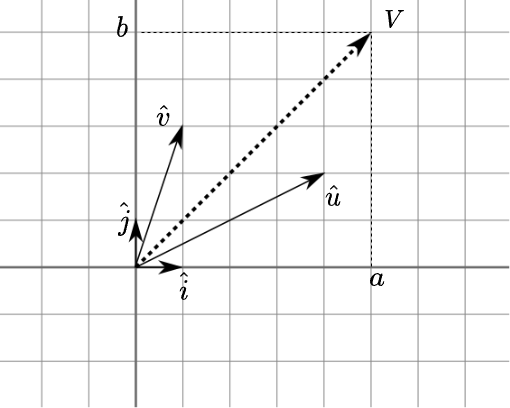
\includegraphics[width=150pt]{../img/ii-span-and-base.png}
        \caption{Figure II.3: Bases of a vector space}
    \end{center}
\end{figure}


We can express \(V = \begin{pmatrix} a \\ b \end{pmatrix}\) as:

\[V = a \hat{i} + b \hat{j}\]

We scale each base vector and add the result to get any vector in the vector space. We can imagine that the base of a vector space are a set of vectors, that fills out the space trough scaling and additions (i.e linear combinations). T

he vector \(V\) in Figure II.3 and any other vector of this vector space, can be also expressed trough a linear combination of \(\hat{u}\) and \(\hat{v}\). We can say that the set of vectors \(\{\hat{u}\), \(\hat{v}\}\) is also a basis for this vector space, but the coordinates of \(V\) would be \(\begin{pmatrix} 1 \\ 1 \end{pmatrix}\) instead of \(\begin{pmatrix} a \\ b \end{pmatrix}\), because \(V = 1 \cdot \hat{u} + 1 \cdot \hat{v}\).

\textbf{Span\index{Span}} of a set of vectors with same dimensions \(n\) is the vector space that can be covered trough the linear combination of the vectors. As we have seen, if all the vectors are linearly independent, they will constitute the basis of an \(n\) dimensional vector space. If only \(p\) vectors are linearly independent and the rest of \(n - p\) vectors can be expressed as linear combination of the other vectors, the span will be a \(p\) dimensional vector space. Two vectors \(\hat{a}\) and \(\hat{b}\) in three dimensions might span a plane if they are linearly independent, a line if they are linearly dependent (\(\hat{a} = c \cdot \hat{b}\) for some scalar \(c\)) or the span might be the point of origin if \(\hat{a} = \hat{b} = \begin{pmatrix} 0 \\ 0 \\ 0 \end{pmatrix}\)

\section{Matrices}

The most important operation in linear algebra are linear transformations. Linear transformation is a way to change all vectors of a vector space according to a linear operator. Transformations on a vector space can be non linear as well, where we can bend or apply some wave to the space, but linear transformation have two properties

\begin{itemize}
    \item Linear transformation does not change the origin of space
    \item Any line in the original space retains it's shape as line in the transformed shape (there is no bending)
\end{itemize}

With these constraints the mathematics of linear transformations are more simple, and faster to compute, but still very useful. To apply linear transformation matrices are used. A matrix \(M_{n,m}\) is a two dimensional structure, noted as a grid

\[M_{n,m} =  \begin{pmatrix}
  x_{1,1} & x_{1,2} & \cdots & x_{1,p} \\
  x_{2,1} & x_{2,2} & \cdots & x_{2,p} \\
  \vdots  & \vdots  & \ddots & \vdots  \\
  x_{n,1} & x_{n,2} & \cdots & x_{n,p}
 \end{pmatrix}\]

Where \(x_{1...n,1...m}\) are real numbers. The set of all matrices of size \(n \cdot m\) containing real numbers is noted with \(\mathbb{R}^{n \cdot m}\).

\subsection{Square matrix}

To understand the structure of transformation matrix, let's start with a certain type of matrix, where the number of rows and columns are equal, called \textbf{square matrix\index{square matrix}}, which we can note \(M_{n, n}\). Such a matrix describes the linear transformation in an \(n\) dimensional vector space with both input and output vectors having \(n\) dimensions.

Linear transformation is interpreted as transforming any or all vector of a vector space. To see the effect of transforming the \(k\) th dimension, we can take the \(k\) th standard basis vector, where each element is \(0\) except for the \(k\) th element, which is 1, and calculate where it would be in the transformed space.

\[\vec i_k = \begin{pmatrix} 0 \\ \vdots \\ 0 \\ 1 \\ 0 \\  \vdots \\ 0 \end{pmatrix} \rightarrow \vec b_k = \begin{pmatrix} b_{k,1} \\ \vdots \\ b_{k,k-1} \\ b_{k,k} \\ b_{k,k+1} \\ \vdots \\ b_{k,n} \end{pmatrix} \]

We can imagine that each column of a matrix is a vector, the matrix \(M_{n, n}\) has \(n\) vectors, each of \(n\) dimensions. The transformation matrix is simply the matrix constructed by conbining all the transformed basis vectors we would get applying the linear transformation to each of the original standard basis vectors.

\begin{equation}I_{n, n} = \begin{pmatrix}
  1 & 0 & \cdots & 0 \\
  0 & 1 & \cdots & 0 \\
  \vdots  & \vdots  & \ddots & \vdots  \\
  0 & 0 & \cdots & 1
 \end{pmatrix} \rightarrow M_{m,n} = \begin{pmatrix}
  b_{1,1} & b_{1,2} & \cdots & b_{1,n} \\
  b_{2,1} & b_{2,2} & \cdots & b_{2,n} \\
  \vdots  & \vdots  & \ddots & \vdots  \\
  b_{n,1} & b_{n,2} & \cdots & b_{n,n}
 \end{pmatrix} \tag{II.1}\end{equation}

To calculate the linear transformation of a vector we use the transformation matrix and we apply an operation called matrix-vector multiplication defined as:

\begin{equation}\begin{aligned}V_t &= M_{n,n} \cdot V \\ &= \begin{pmatrix}
  x_{1,1} & x_{1,2} & \cdots & x_{1,n} \\
  x_{2,1} & x_{2,2} & \cdots & x_{2,n} \\
  \vdots  & \vdots  & \ddots & \vdots  \\
  x_{n,1} & x_{n,2} & \cdots & x_{n,n}
 \end{pmatrix} \begin{pmatrix} v_1 \\ v_2 \\ \vdots \\ v_n \end{pmatrix} \\ &= v_1\begin{pmatrix}
  x_{1,1} \\ x_{2,1} \\ \vdots \\ x_{n,1} \end{pmatrix} + v_2\begin{pmatrix}
  x_{1,2} \\ x_{2,2} \\ \vdots \\ x_{n,2} \end{pmatrix} + ... + v_n\begin{pmatrix}
  x_{1,n} \\ x_{2,n} \\ \vdots \\ x_{n,n} \end{pmatrix} \\ &= \begin{pmatrix}
  x_{1,1} v_1 + x_{1,2} v_2 + \cdots + x_{1,n} v_n  \\
  x_{2,1} v_1 + x_{2,2} v_2 + \cdots + x_{2,n} v_n  \\
  \vdots \\
  x_{n,1} v_1 + x_{n,2} v_2 + \cdots + x_{n,n} v_n  \\
 \end{pmatrix}\end{aligned}\tag{II.2}\end{equation}

The resulting vector \(V_t\) is also \(n\) dimensional. The matrix \(I_{n, n}\) in Figure II.1 is called the identity matrix. If we use this matrix as a transformation operator for a vector \(V\), it would result in the same vector \(I_{n,n} \cdot V = V\).


\begin{figure}[htbp]
    \begin{center}
        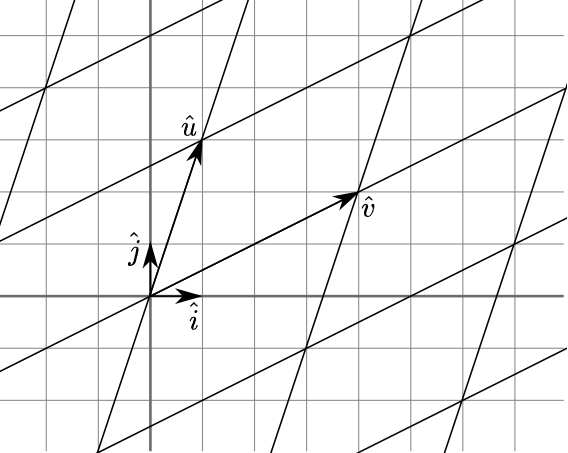
\includegraphics[width=150pt]{../img/ii-matrix.png}
        \caption{Figure II.4: Vector space transformation}
    \end{center}
\end{figure}


In Figure II.4 we can see the visual representation of a two dimensional vector space transformation. The standard base of the original space is \(\{\vec i, \vec j\}\) and it's shown as a gray grid. The transformed space has standard base \(\{\vec u, \vec v\}\), these vectors correspond to \(\vec i\) and \(\vec j\) in the original vector space. We can imagine that the space is stretched so that \(\vec i\) and \(\vec j\) are moved to the place of \(\vec u\) and \(\vec v\).

\[\vec i \rightarrow \vec u, \vec j \rightarrow \vec v\]

In Figure II.4 the transformed space can be seen as an elongated diagonally skewed grid of black lines. This transformation is described by a \(2 \cdot 2\) matrix, having first column the elements of vector \(u\) and second columns with elements of vector \(v\).

\[M_{uv} = \begin{pmatrix}
  u_{1} & v_{1} \\
  u_{2} & v_{2}
 \end{pmatrix}\]

If we apply the matrix-vector multiplication in the Formula II.2 to the matrix \(M_{2,2}\) and \(\vec i\), we get \(\vec u\):

\[M_{uv} \cdot \vec i = \begin{pmatrix}
  u_{1} & v_{1} \\
  u_{2} & v_{2}
 \end{pmatrix} \begin{pmatrix} 1 \\ 0 \end{pmatrix} =
 \begin{pmatrix} 1 \cdot u_{1} + 0 \cdot v_{1} \\ 1 \cdot u_{2} + 0 \cdot v_{2} \end{pmatrix} = \vec u\]

Similarly we can show that \(\vec j \rightarrow \vec v\). \(M_{2,2}\) similarly transforms all vectors in the space.


\begin{figure}[htbp]
    \begin{center}
        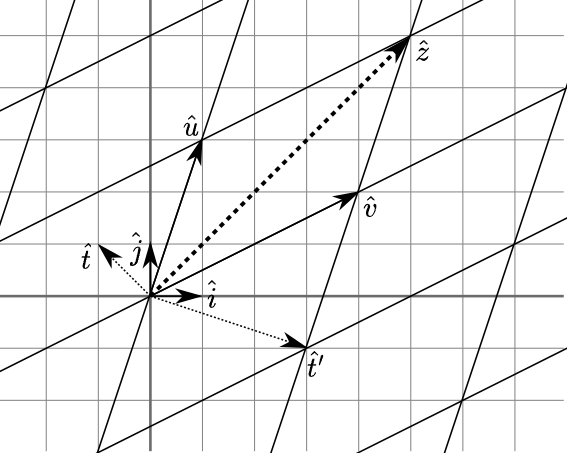
\includegraphics[width=150pt]{../img/ii-matrix-2.png}
        \caption{Figure II.5: The transformation applied to a vector}
    \end{center}
\end{figure}


Figure II.5 shows the effect of applying the linear transformation of our example matrix \(M_{uv}\) on vector \(\vec t\), resulting in vector \(\vec t'\). We can see that the vector space was not only elongated but also flipped around the axis of vector \(\vec z\)

\subsection{Determinant}

A transformation might expand or condense the vector space. The \textbf{determinant\index{determinant}} of a matrix measures the rate of expansion applied to a vector space by the matrix.

The standard basis vectors (what we noted with \(\vec i_k, k = 1..n\)) define a \(1 \times 1 \times ... \times 1\) hypercube, where each standard basis vector would be an edge of the cube around the corner where the origin \(O\) is. If we apply the linear transformation defined by the matrix to this cube, we get a shape called \textbf{parallelotope\index{parallelotope}} (parallelogram in 2D, parallelepiped in 3D). The determinant is the area of the resulting shape after applying the matrix transformation. The determinant will be the same if we apply the transformation to any \(n\) dimensional hypercube in the vector space. Any shape that can be approximated with such hypercubes will also scale with the same factor. The determinant is only defined for square matrices.

The determinant can have the following meaning depending on it's value:
\begin{itemize}
    \item Determinant of \(1\) means there is no change in the area of hypercube when applying the matrix transformation. This is the case for example for rotation and \textbf{sheer\index{sheer}} operation.
    \item A determinant of \(0\) of a matrix means the area of the hypercube is scaled down to \(0\) with the matrix transformation. This is called \textbf{projection\index{projection}}, we reduce one or more dimension by projecting all points of our hyperspace to a lower dimension hyperplane or all the way down the point of origin. This also means that some or all vectors from the matrix columns are linearly dependent, based on how many dimensions we reduce.
\end{itemize}

    The number of linearly independent columns (taken as vectors) in a square matrix is called the \textbf{rank\index{rank}} of the matrix. Rank is also the number of dimensions of the hyperplane resulting when applying the matrix transformation to our vector space. If the rank is equal to the number of columns, the determinant is not \(0\).

    In the case of a projection a line or a hyperplane or the entire hyperspace will be projected to the point of origin \(O\). The line, plane or hyperspace that ends up as the origin after the transformation is called the \textbf{kernel\index{kernel}} or \textbf{null space\index{null space}} of the matrix. Mathematically the kernel is defined as the set of all vectors that become null vectors after the matrix transformation

    \begin{equation}N(M)=\{v|M \vec v=\vec 0\} \tag{II.3}\end{equation}
\begin{itemize}
    \item The determinant will be negative for one or any odd number of flips in the hyperspace. An even number of flips restores the space to it's original "side", the same transformation can be achieved trough rotation. The absolute value of a negative determinant will tell the factor the space is being scaled.
\end{itemize}

The computation itself for the determinant is more complex for each added dimension, but here we will explore the two dimensional case and it's computation.


\begin{figure}[htbp]
    \begin{center}
        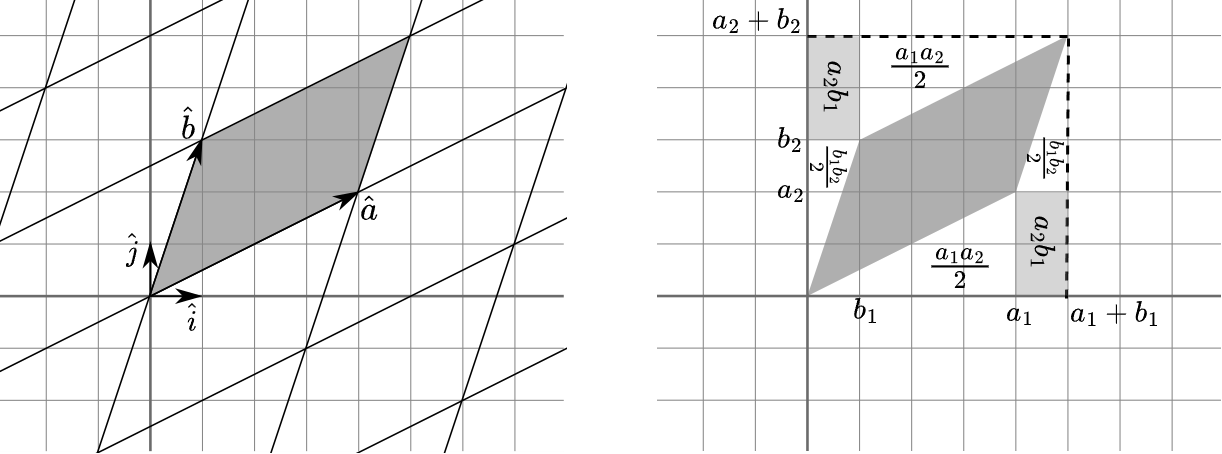
\includegraphics[width=250pt]{../img/ii-determinant.png}
        \caption{Figure II.6: Determinant of a matrix}
    \end{center}
\end{figure}


In Figure II.6 we can see two vectors of \(\vec a = \begin{pmatrix} a_1 \\ a_2 \end{pmatrix}\) and \(\vec b = \begin{pmatrix} b_1 \\ b_2 \end{pmatrix}\). They can form the transformation matrix \(M_{ab} =  \begin{pmatrix}
  a_{1} & b_{1} \\
  a_{2} & b_{2}
 \end{pmatrix}\). If we apply \(M\) as the transformation matrix to the basis \(\{\vec i, \vec j\}\) we get the new basis \(\{\vec a, \vec b\}\). The area of the \(1 \times 1\) square resting on the \(\{\vec i, \vec j\}\) becomes the shaded area resting on \(\{\vec a, \vec b\}\). The determinant of the matrix \(M\) is the resulting area:

 \[\det(M_{ab}) = \det\begin{pmatrix}
  a_{1} & b_{1} \\
  a_{2} & b_{2}
 \end{pmatrix} = a_1b_2 - b_1a_2\]

This can be derived looking at the right side of Figure II.6:

\(\det(M_{ab}) = (a_1 + b_1)(a_2 + b_2) - 2 {a_1a_2 \over 2}  - 2 {b_1b_2 \over 2} - 2 a_2 b_1\) \\
\(= a_1a_2 + a_1b_2 + a_2b_1 + b_1b_2 - a_1a_2 - b_1b_2 - 2 a_2 b_1\) \\
\(= a_1b_2 - a_2b_1\)

If we create another matrix with the columns flipped \(M_{ba} = \begin{pmatrix}
  b_{1} & a_{1} \\
  b_{2} & a_{2}
 \end{pmatrix}\) this would not only scale the vector space but also flip as we have seen in the case of \(M_{uv}\) flipping the space around \(\vec z\), on Figure II.5. In this case the determinant is negative, but absolute value remains the same:

 \[\det(M_{ab}) = -\det(M_{ba})\]

\subsection{Special transformations with square matrices}

Depending on the type of transformation we can define some special matrices

\begin{itemize}
    \item \textbf{Identity matrix\index{Identity matrix}} \(I_{n,n}\) has values of \(1\) on it's diagonal and \(0\) on every other, off-diagonal element. We have seen that this matrix preserves all vectors without any transformation.
\end{itemize}

\begin{itemize}
    \item \textbf{Scalar matrix\index{Scalar matrix}} has values of \(k\) on it's diagonal and \(0\) on every other, off-diagonal element. We can express a scalar matrix as \(kI_{n,n}\). What this matrix does is scales the vector space by a scale of \(k\). For values \(k > 1\) the vector space is expanded, for values in the interval \((0, 1)\), the space is shrunk, for negative values of \(k\) the space is mirrored around the origin and scaled by a factor of \(k\).
\end{itemize}

\begin{itemize}
    \item \textbf{Scaling along a single dimension\index{Scaling along a single dimension}} can be done with a matrix where all elements are same as the identity matrix, but a single element on the diagonal has a scaler value of \(k\). This matrix will preserve sizer on all dimension except for the modified dimension, where a scale by \(k\) will be applied. Setting a diagonal element to \(-1\) will mirror around that dimension.
\end{itemize}

\begin{itemize}
    \item \textbf{Shear operation\index{Shear operation}} is a matrix which is same as an identity matrix, except a single off-diagonal element, which is a non zero \(k\) real number. For example in two dimensions a sheer matrix \(S = \begin{pmatrix}
1 & k \\
0 & 1
\end{pmatrix}\). Shear matrices have a determinant of \(1\)
\end{itemize}

\begin{itemize}
    \item \textbf{Orthogonal matrix\index{Orthogonal matrix}} is a matrix whose vectors fulfill two conditions:
            \begin{itemize}
            \item each vector in the matrix (column) has a norm of 1
            \item all vectors in the matrix are orthogonal to each other (dot product between any two columns are \(0\))
        \end{itemize}
\end{itemize}

    This means each vector has size \(1\) and perpendicular to all the other vectors. The identity matrix \(I_{n,n}\) and any other matrix which is a rotation or mirroring in \(n\) dimensions of the identity matrix are orthogonal. Applying this matrix as a transformation will result in rotation or mirroring or a combination of both.

\begin{itemize}
    \item \textbf{Proper orthogonal matrix\index{Proper orthogonal matrix}} adds one more condition to orthogonal matrix, that the angles of vectors are preserved. This can be verified by a determinant of \(1\). Proper orthogonal matrix will apply a rotation around the origin to the vector space without mirroring. As we have mentioned, mirroring even number of times results in a transformation which is same as a rotation.
\end{itemize}

These transformation can be applied to images as well, where we can calculate the position of each pixel in a resulting image and apply interpolation or smoothing to fill in the gaps. An exception might be rotation, which is mostly done using a system called \textbf{quaternions\index{quaternions}}. Rotation with matrices suffer from a limitation called gimbal locks, where angles can align and lose degrees of freedom. Combined with limited precision of float representation of numbers, results in highly unstable motion. Quaternions use a four dimensional unit hyper-sphere to describe rotation in three dimensions.

\subsection{Nonsquare matrices}

A square matrix with \(n\) rows and \(n\) columns applies a transformation in an \(n\) dimensional vector space. A matrix with \(n\) columns and \(m\) rows makes a transformation from an \(n\) to an \(m\) dimensional space. The input is an \(n\) dimensional vector and the output is an \(m\) dimensional vector.

When \(m < n\), it's called a projection. When \(m > n\) the result is higher dimension, but because matrices describe linear transformation, the result of the transformation remains an \(n\) dimensional hyper plane in the \(m\) dimensional space.

Matrix transformation is done similarly to square matrices.

\[\begin{aligned}V_m &= M_{m,n} \cdot V_n \\ &= \begin{pmatrix}
  x_{1,1} & x_{1,2} & \cdots & x_{1,n} \\
  x_{2,1} & x_{2,2} & \cdots & x_{2,n} \\
  \vdots  & \vdots  & \ddots & \vdots  \\
  x_{m,1} & x_{m,2} & \cdots & x_{m,n}
 \end{pmatrix} \begin{pmatrix} v_1 \\ v_2 \\ \vdots \\ v_n \end{pmatrix} \\ &= \begin{pmatrix}
  x_{1,1} v_1 + x_{1,2} v_2 + \cdots + x_{1,n} v_n  \\
  x_{2,1} v_1 + x_{2,2} v_2 + \cdots + x_{2,n} v_n  \\
  \vdots \\
  x_{m,1} v_1 + x_{m,2} v_2 + \cdots + x_{m,n} v_n  \\
 \end{pmatrix}\end{aligned}\]

\subsection{Matrix multiplication}

Matrices, which describe linear transformations in vector spaces, can be combined. We can express as a single matrix the transformation described by the matrix \(B\) happening after a transformation described by the \(A\). This is called \textbf{composition\index{composition}} of two transformations and the mathematical operation for composition is \textbf{matrix multiplication\index{matrix multiplication}}: \(B \cdot A\). When we apply a matrix as a transformation to a vector \(AV\) we put the matrix on the right hand side, we can imagine that composition is \(B(AV) = BAV\). We can remove the parenthesis because matrix multiplication is associative: the same transformations are being applied in the same order even if we evaluate the multiplications in different orders. This notation of inversed order come from function notations \(g(f(x))\)

The formula for matrix multiplication uses the formula of matrix vector multiplication (Formula II.2). Each column \(k\) in the output matrix, if treated as a vector, is the \(k\) th column in the right hand side matrix, also treated as a vector, transformed  (multiplied) by the left hand matrix. Summarized the product formula looks like this:

\[\begin{aligned}B \cdot A &= \begin{pmatrix}
  b_{1,1} & b_{1,2} & \cdots & b_{1,m} \\
  b_{2,1} & b_{2,2} & \cdots & b_{2,m} \\
  \vdots  & \vdots  & \ddots & \vdots  \\
  b_{p,1} & b_{p,2} & \cdots & b_{p,m}
 \end{pmatrix}\begin{pmatrix}
  a_{1,1} & a_{1,2} & \cdots & a_{1,n} \\
  a_{2,1} & a_{2,2} & \cdots & a_{2,n} \\
  \vdots  & \vdots  & \ddots & \vdots  \\
  a_{m,1} & a_{m,2} & \cdots & a_{m,n}
 \end{pmatrix}\\ &= \begin{pmatrix}
  \sum_{i=1}^m b_{1,i}a_{i,1} & \sum_{i=1}^m b_{1,i}a_{i,2} & \cdots & \sum_{i=1}^m b_{1,i}a_{i,n} \\
  \sum_{i=1}^m b_{2,i}a_{i,1} & \sum_{i=1}^m b_{2,i}a_{i,2} & \cdots & \sum_{i=1}^m b_{2,i}a_{i,n} \\
  \vdots  & \vdots  & \ddots & \vdots  \\
  \sum_{i=1}^m b_{p,i}a_{i,1} & \sum_{i=1}^m b_{p,i}a_{i,2} & \cdots & \sum_{i=1}^m b_{p,i}a_{i,n}
 \end{pmatrix}\end{aligned}\]

Matrices can be multiplied only if the number of columns of the left hand matrix \(m\) is equal to the number of rows to the right hand matrix: the output dimension of the first transformation has to be the same as the input dimension of the second transformation. The input dimension of the product \(B \cdot A\) is the number of columns \(n\) of the right hand side matrix \(A\), the output dimension is the number of rows \(p\) in the left hand matrix \(B\).

Matrix multiplication is not commutative. For non square matrices, the input-output dimensions need to match up, but for square matrices depending on the order of transformations applied, the result might be different:

\[\exists A, B \in R^{n,n} \rightarrow B A \neq A B\]

In case of square matrices, the determinant of matrix multiplication is equal to the product of the determinants:

\[\det(B \cdot A) = \det(B) \det(A)\]

While the mathematical proof of this is difficult, the intuition behind this is that the rate of change \(\det(B \cdot A)\) on the vector space described by the composite transformation \(B \cdot A\) is same as the rate of change \(\det(B)\) done by the matrix \(B\) on the rate of change \(\det(A)\) done by \(A\).

\subsection{Inverse matrices}

As matrices describe transformations, the inverse of a transformation can be described by the \textbf{inverse matrix\index{inverse matrix}}. We note inverse matrix of \(M\) with \(M^{-1}\):

\[M^{-1}M = MM^{-1} = I\]

Applying both \(M\) and the inverse \(M^{-1}\) is equivalent to applying the identity matrix as a transformation.

Projections don't have a defined inverse (there is loss of information, e.g the matrix might project every line to a point, so the inverse would be expanding a point to a line, which cannot be done with a linear operation, so non square matrices don't have definition of inverse matrices. Similarly we have seen that determinant of \(0\) also constitutes as projection, so matrices with \(\det(M) = 0\) also do not have an inverse matrix defined.

Several highly optimized algorithms have been proposed to calculate the inverse. In many cases, the inverse matrix is not even calculated, rather the operation done with the inverse matrix (e.g matrix vector multiplication) is calculated or approximated trough an iterative process. This approach saves computation as well as memory for large matrices.

\subsection{Change of basis}

In the same way we applied a matrix as a transformation to a vector in a vector space, we can apply a matrix as a transformation to the base of the vector space as well. Transforming the vector to another basis is done the same way as applying transformation to the vector.

\[U = B \cdot V\]

where \(V\) is the vector, \(B\) is the transformation matrix and \(U\) is the vector \(V\) under the basis \(B\) (it's the same equation as transforming \(V\) by \(B\), but different interpretation).

In some cases transforming a vector under a specific base is more simple than in another base. A common process in linear algebra is to transform a vector to another base (noted with \(B\)), apply a specific transformation under the base of \(B\) (noted with \(M_B\)), and reverse the base transformation. A transformation can be reversed using the inverse matrix \(B^{-1}\):

\[U = B^{-1} \cdot M_B \cdot B \cdot V\]

In the above there are the following steps, which we can read right to left:
\begin{itemize}
    \item Transform \(V\) to another basis with \(B\)
    \item Apply matrix transformation using \(M_B\)
    \item Reverse basis transformation with \(B^{-1}\)
\end{itemize}

All the above steps are simple matrix multiplications.

\subsection{Eigenvectors and eigenvalues}

The hyperline a non-zero vector rests on is the \textbf{span\index{span}} of the vector. When we apply a matrix transformation to all vectors of a vector space, most vectors would change direction where they point, we say they \textbf{change their span\index{change their span}}. This definition of span is a unique case of the definition highlighted above, applied to a single vector.

\textbf{Eigenvectors\index{Eigenvectors}} of a matrix \(M\) which do not change their span during the matrix transformation. Eigenvectors might change scale during the matrix transformation, the rate of change \(\lambda\) is called the \textbf{eigenvalue\index{eigenvalue}} of the eigenvector.

The mathematical relationship is defined as:

\begin{equation}MV = \lambda V \tag{II.4}\end{equation}

which states that applying the matrix \(M\) as a linear transformation to \(V\) is same as multiplying \(V\) with a scalar \(\lambda\). While this equation is not true for all vectors, all non zero solutions of \(V\) are the eigenvectors and corresponding result of \(\lambda\) are the eigenvalues. We can rearrange the equation by introducing the identity matrix on the right side and moving everything to the left, resulting in the zero vector \(\vec 0\) :

\[MV - I \lambda V = \vec 0 \\
(M- I\lambda) V = \vec 0\]

Writing the above in detail:

\[\begin{pmatrix}
  m_{1,1} - \lambda & m_{1,2} & \cdots & m_{1,n} \\
  m_{2,1} & m_{2,2} - \lambda & \cdots & m_{2,n} \\
  \vdots  & \vdots  & \ddots & \vdots  \\
  m_{n,1} & m_{n,2} & \cdots & m_{n,n} - \lambda
 \end{pmatrix} \begin{pmatrix} v_{1} \\  v_{2} \\  \vdots\\ v_{n} \end{pmatrix}
= \begin{pmatrix} 0 \\ 0 \\  \vdots\\ 0 \end{pmatrix} \]

The result of \((M- I\lambda) V\), a matrix vector multiplication has to be \(\vec 0\), meaning the matrix \(M- I\lambda\) reduces the dimension of the vector space, which in turn is only possible if the determinant is \(0\): \(det(M- I\lambda) = 0\). We can use this property together with the equation of determinant to calculate the eigenvalues and eigenvectors of a matrix. A polinomial \(O(n^3)\) algorithm exists for calculating the determinant which in turn is an n-th degree polynomial, having \(n\) solutions for the eigenvalue \(\lambda\).  Using solutions of \(\lambda\) in Equation II.4 we can get eigenvectors for each eigenvalue up to a constant factor, meaning that we will not get an exact vector, only a direction. Since all vectors on the direction of an eigenvector will share the properties of preserving the span and be scaled by a constant, so they are also eigenvectors. In other words if we multiply an eigenvector \(\vec e\) with a constant \(c\) we get another eigenvector \(\vec e'\):

\[\vec e' = c \vec e\]

Since in most cases we need a single eigenvector per direction, we can use the normalized version (length \(1\)), and because we still have two of these, for the case of \(c = -1\), we can choose the one where the first element is always positive.

Figure II.7 displays a two dimensional example of the eigenvector and eigenvalue. On the left side we see two vectors \(\vec e_1\) and \(\vec e_2\), and the lines on which the vectors rest on. The lines are the spans of the vectors. On the right side of the diagram we have two more vectors, \(\vec a = \begin{pmatrix} a_1 \\ a_2 \end{pmatrix}\) and \(\vec b = \begin{pmatrix} b_1 \\ b_2 \end{pmatrix}\). The vectors \(\vec a\) and \(\vec b\) can describe a transformation as \(M = \begin{pmatrix}a_{1} & b_{1} \\ a_{2} & b_{2}\end{pmatrix}\). Applying the transformation \(M\) would knock any vector off it's span in our two dimensional vector space except for vectors resting on the two highlighted lines.


\begin{figure}[htbp]
    \begin{center}
        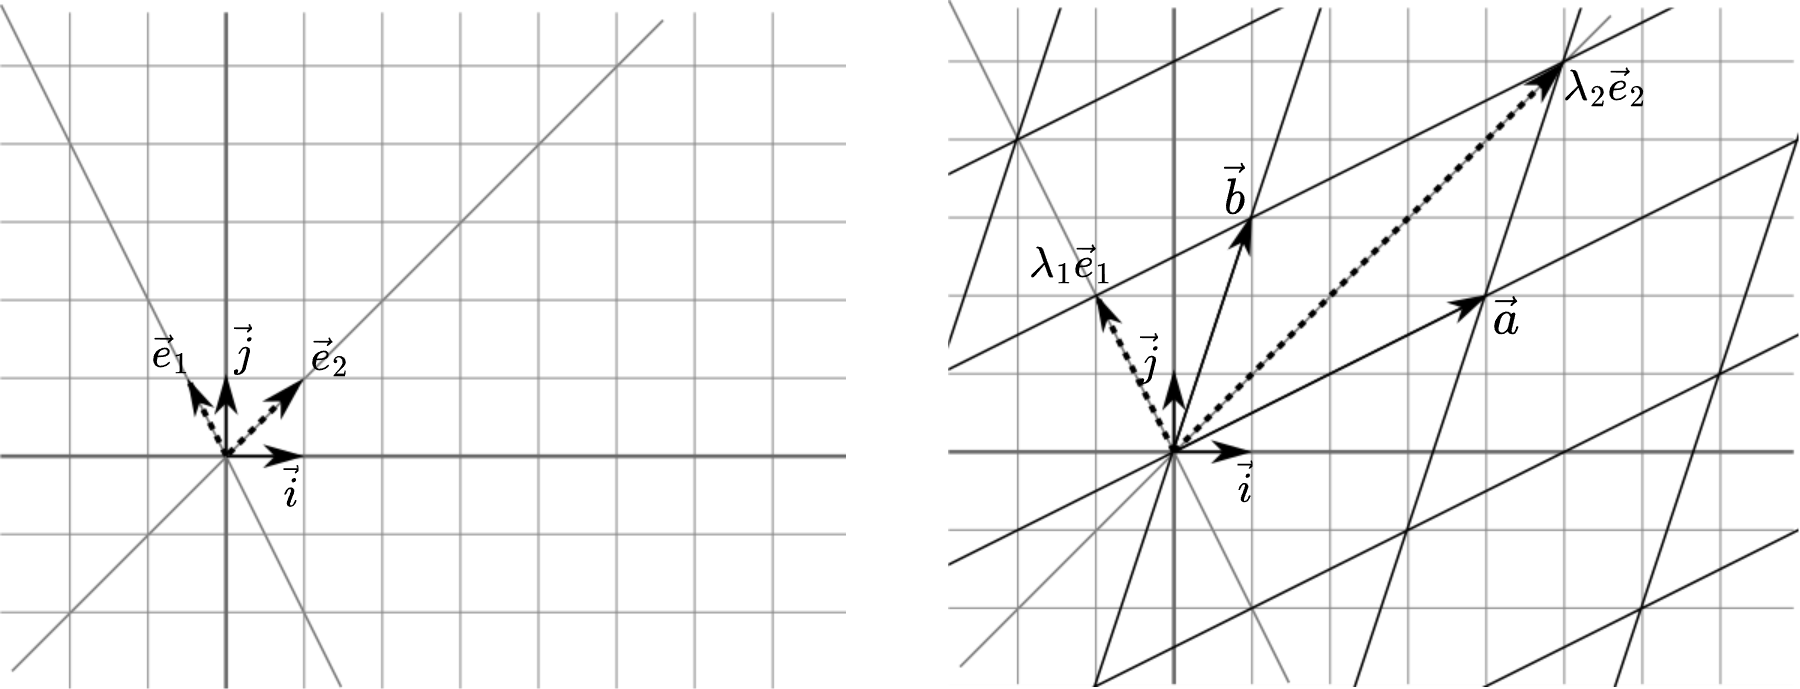
\includegraphics[width=300pt]{../img/ii-eigen.png}
        \caption{Figure II.7: Eigenvectors and eigenvalues of a transformation}
    \end{center}
\end{figure}


\(\vec e_1\) and \(\vec e_2\) are eigenvectors of \(M\), applying \(M\) as a matrix transformation to these vectors we get \(\lambda_1 \vec e_1\) and \(\lambda_2 \vec e_2\) respectively, meaning their span was preserved and they were scaled by the eigenvalues \(\lambda_1\) and \(\lambda_2\). All vectors on the highlighted spans are eigenvectors.

A special case is scaler transformation matrices (matrices that apply scaling on the vector space). When we apply a scaling matrix, all vectors of a vector space will preserve their span. In this case all vectors in the vector space are eigenvectors belonging to a single eigen value, which is the same as the scaling applied by the matrix.

Another special case is rotation. Rotation in two dimensions will knock all vectors off their span except the \(\vec 0\). Since eigenvector needs to be non zero, a two dimensional rotation does not have any eigenvector. In three dimension, applying a rotation matrix, the span of the resulting eigenvector will define the axis of rotation. The corresponding eigenvalue would be \(1\) since there is no scaling.

\section{Matrix decomposition}

Matrix multiplication is also called composition, because we are composing multiple transformations into a single one. Given a matrix, \textbf{decomposition\index{decomposition}} of the matrix means writing a matrix in terms of the product of other matrices. The geometric interpretation is that we rewrite a linear transformation as a series of transformations, usually more simple ones. In most cases our aim is for each matrix in our decomposition to be a primitive operation like a rotation or scaling. While composition gives a single result, decomposition can be done in infinite ways.

\subsection{Eigen decomposition}

\textbf{Eigen decomposition\index{Eigen decomposition}} decomposes a matrix into three transformation using eigenvectors usinng the formula for basis change:

\begin{itemize}
    \item Change basis to the base defined by eigenvectors
    \item Apply simple scaling
    \item Reverse base change
\end{itemize}

Eigen decomposition can only be applied in the following conditions:

\begin{itemize}
    \item The matrix we want to decompose is a square matrix. Only square matrices have eigenvalues
    \item The \(n\) dimensional matrix has \(n\) eigenvalues with \(n\) corresponding linearly independent eigenvectors. This is required for inverse matrix part of the basis change.
\end{itemize}

We will decompose a square matrix \(A\) with \(e_1...e_n\) as the normalized, linearly independent eigenvectors of \(A\) and \(\lambda_1...\lambda_n\) as the corresponding eigenvalues. Using the formula for eigenvalues and eigenvectors we can write \(n\) equations in the form:

\[Ae_1 = \lambda_1 e_1 \\ Ae_2 = \lambda_2 e_2 \\ ... \\ Ae_n = \lambda_n e_n\]

We can rewrite our \(n\) equation using a single matrix equation:

\[A\begin{pmatrix}
  | & | &  & | \\
  e_1 & e_2 & \cdots & e_n \\
  | & | &  & | \\
 \end{pmatrix} = \begin{pmatrix}
  | & | &  & | \\
  e_1 & e_2 & \cdots & e_n \\
  | & | &  & | \\
 \end{pmatrix}\begin{pmatrix}
  \lambda_1 & 0 & \cdots & 0 \\
  0 & \lambda_2 & \cdots & 0 \\
  \vdots  & \vdots  & \ddots & \vdots  \\
  0 & 0 & \cdots & \lambda_n
 \end{pmatrix}\]

To see that this is true we can apply the matrix multiplication. If we name the matrix where each column is an eigenvector with \(U\) and the column matrix with eigenvalues \(\Lambda\) we can rewrite the equation as:

\[AU = U\Lambda\]

Applying \(U^{-1}\) from the right to both sides we get the formula for eigen decomposition

\begin{equation}A = U\Lambda U^{-1} \tag{II.5}\end{equation}

\(\Lambda\) is a column matrix, which corresponds to a scaling transformation. Formula II.5 corresponds to a basis change, and applying a simple scaling in the modified basis.

One very useful use case of eigen decomposition is calculating large powers of a matrix. We can rewrite \(A^k\) as:\\
\(A^k = U \Lambda U^{-1} \cdot U\Lambda U^{-1}  \cdot ...  \cdot U\Lambda U^{-1}\)

The \(U^{-1} \cdot U\) pairs cancel out giving\\
\(A^k = U \Lambda^k U^{-1}\)

Where \(\Lambda^k\) can be calculated with much fewer operations, having the form of:

\(\Lambda^k = \begin{pmatrix}
  \lambda_1^k & 0 & \cdots & 0 \\
  0 & \lambda_2^k & \cdots & 0 \\
  \vdots  & \vdots  & \ddots & \vdots  \\
  0 & 0 & \cdots & \lambda_n^k
 \end{pmatrix}\)

While \(U\) and \(U^{-1}\) also require computation, for high power of \(k\) the eigen decompostion might be computationally less heavy, more so if results for multiple powers of \(k\) are needed. Another use case is if we apply to special matrices where computing \(U^{-1}\) from \(U\) is straightforward.

\subsection{Transpose of a matrix}

Before we look into other decompositions we need the definition of a new operator: \textbf{transpose of a matrix\index{transpose of a matrix}}.

While transpose of a matrix does not have a simple and intuitive geometric interpretation, the mathematical definition is quite simple. The transpose of a matrix is an operation that flips the matrix over its diagonal, switching the row and column indices. Given a matrix \(A\) of dimensions \(m \times n\), the transpose of \(A\), denoted as \(A^T\) or \(A'\), is a new matrix of dimensions \(n \times m\), where the element at row \(i\) and column \(j\) in \(A\), noted with \(a_{i,j}\), becomes the element at row \(j\) and column \(i\) in \(A^T\), noted with \(a^T_{j,i}\):

\[a_{i,j} = a^T_{j,i}\]

An interesting case of transpose is that of an orthogonal matrix, noted with \(R\), resulting in it's inverse:

\begin{equation}R^T = R^{-1} \tag{II.6}\end{equation}

An orthogonal matrix describes a rotation, the inverse matrix describes the inverse transformation. Inverse of a rotation would mean a rotation in inverse direction with same angle and axis as the original rotation.

Proof of Formula II.6:\\
\(R^T = R^{-1}\) multiply from the right side with \(R\)\\
\(R^TR = R^{-1}R\)\\
\(R^TR = I\)\\
The matrix product is a dot product of columns of the left hand side matrix with rows of the right hand side matrix. Since \(R\) is orthogonal means every column, if treated as a vector, has a norm of \(1\) and is orthogonal to every other column vector, except for itself. Here, we are multiplying the orthogonal matrix with it's transpose, which means we will calculate dot products of orthogonal vectors. The dot product of two orthogonal vectors is \(0\), the dot product of a unit vector with itself is \(1\). This means that elements on the main diagonal would result in \(1\) and elements off the main diagonal would result in \(0\), giving the overall result as \(I\).

We can define transpose of vectors as well, in which case it will turn a single column vector to a single row vector and vice versa. We can use it to more properly define product of perpendicular vectors as

\[U  \cdot V^T = 0\]

where \(U\) and \(V\) are perpendicular vectors.

A property of transpose is that transpose of a product (of vectors and matrices) is the inverse direction of product of element wise transpose:

\begin{equation}(AB)^T = B^TA^T \tag{II.7}\end{equation}

where \(A\) and \(B\) can be matrices or vectors of appropriate sizes to accomodate the definition of product (e.g A may be matrix and B can be a vector).

The transpose of a scalar is simply itself:

\[c^T = c\]

\subsection{Symmetric matrices}

A square matrix \(M\) is \textbf{symmetric\index{symmetric}} if elements \(m_{i,j}\)  below the main diagonal (\(m_{i,i}\)) are equal to their corresponding pair above the main diagonal: \(m_{i,j} = m_{j,i}\) (notice the change of order between \(i\) and \(j\)). Non-square matrices cannot be symmetrical.

Symmetric matrices are very useful because they have lots of favorable properties.

The most simple property is that the transpose of a symmetric matrix is equal to the original matrix.

\[S = S^T \iff S \operatorname{is\ symmetrical}\]

Eigenvectors of symmetric matrices also have very useful properties. Symmetric matrices of dimension \(n\) have \(n\) non zero eigenvalues and \(n\) linearly independent eigenvectors (vectors have unique directions). The proof of this is quite complex involving further definitions we omitted so we will omit the proof of this also.

An even more interesting property which can be easily shown is that the eigenvectors of symmetric matrices are orthogonal. In other words, each eigenvector is perpendicular to all others. And since we can mirror eigenvectors on the point of origin and get a corresponding eigenvector, eigenvectors will form a proper orthogonal basis. Proper orthogonal basis is same as the basis of the vector space rotated away.

Proof:\\

To prove let's consider the symmetric matrix \(A\) and two linearly independent eigenectors \(x\) and \(y\), corresponding to different eigenvalues \(\lambda_x\) and \(\lambda_y\) respectively (instead of two eigenvectors of the same direction, corresponding to same eigenvalue)

Using the definition of eigenvalue and eigenvector we can input our two eigenvalues and corresponding eigenvectors to get two equations:

\(Ax = \lambda_x x,\ Ay = \lambda_y y\)\\
Multiplying with the transpose of the other eigenvector from the left we get\\
\(y^TAx = \lambda_x y^T x,\ x^TAy = \lambda_y x^Ty\)\\
Taking transpose of both sides of the first equation and keeping the second one as is\\
\((y^TAx)^T = (\lambda_x y^T x)^T,\ x^TAy = \lambda_y x^Ty\)\\
Apply itemwise transpose instead of transpose of product\\
\((x^T)^TA^Ty = \lambda_x x^T y,\ x^TAy = \lambda_y x^Ty\)\\
Transpose of a transpose of a vector is same as the vector (we just turn column vector to row and back to column). Also transpose of a symmetric matrix is itself and \(A\) is symmetric:\\
\(x^TAy = \lambda_x x^T y,\ x^TAy = \lambda_y x^Ty\)\\
The left hand side of both equations are now equal, we can substract the two equations:\\
\(0 = (\lambda_x - \lambda_y)x^Ty\)\\
And since we said that \(\lambda_x \ne \lambda_y\) and the vectors \(x\) and \(y\) are non zero, it must be that \(x^Ty = 0\) which is the definition of orthogonal vectors.

\subsection{Spectral decomposition}

\textbf{Spectral decomposition\index{Spectral decomposition}} is the process of applying eigen decomposition to symmetric matrices using the properties discussed earlier. The eigenvectors of a symmetric matrix are orthogonal (perpendicular), and describe a new basis. We can change the basis from the symmetric matrix trough a simple rotation to the basis described by the eigenvectors. As we have seen for eigen decompostion, the transformation becomes a simple scaling under the base of eigenvectors. Writing all this mathematically we get the decomposition of a symmetric matrix \(S\) as:

\[S = Q\ \Lambda\ Q^T\]

where \(Q\) is an orthogonal matrix we use to change basis, but using transpose to change back, instead of inverse, because they are equal. Each column of \(Q\) is a normalized eigenvector of \(S\). \(\Lambda\) is a diagonal matrix describing a simple scaling operation under the changed basis. The values on the diagonal of \(\Lambda\) are the eigenvalues of \(S\).

Spectral decomposition states that all symmetric matrices can be decomposed as a rotation, which we can calculate by finding the normalized eigenvectors, a scaling and an inverse rotation given by the transpose of the rotation.

\subsection{Singular value decomposition (SVD)}

So far we looked into eigenvalue decomposition which could be applied to matrices with certain conditions. Than we have seen spectral decomposiotn which was a special case of eigen decomposition, applied to an even more specific matrix, the symmetric matrix.

\textbf{Singular Value Decomposition (SVD)\index{Singular Value Decomposition (SVD)}} is a powerful matrix decomposition technique, and the beautiful thing about it is its generality. SVD can be applied to any \(m \times n\) matrix.

While most matrices  are not symmetrical we can construct symmetric matrices for any matrix. Given an \(m \times n\) matrix \(A\) both \(AA^T\) of size \(m\times m\) and \(A^TA\) of size \(n \times n\) are symmetrical. This statement is very simple to prove, using the attribute that the transpose of a product is the inverse ordered product of element wise transpose (Equation II.7). Using this attribute we can show that the transpose of the product \(AA^T\) is same as itself. First we apply Formula II.7 to \(AA^T\)\\

\((AA^T)^T = (A^T)^TA^T\)\\
And than we simplify \((A^T)^T = A\)\\
\((AA^T)^T = AA^T\)\\

Since the expression \(AA^T\) is equal to it's transpose \((AA^T)^T\), it means \(AA^T\) is symmetrical. Similarly we can show that \(A^TA\) is also symmetrical. We can name \(AA^T\) as \(S_L\) (left) and \(A^TA\) as \(S_R\) (right).

\(S_L\) and \(S_R\), because they are product in the form of \(MM^T\), are not only symmetric matrices but all eigenvalues are non negative, also called \textbf{positive semi-definite\index{positive semi-definite}} (PSD) matrices. Furthermore if we sort eigenvalues of \(S_L\) and \(S_R\) in decreasing order, the largest eigenvalue of both matrices will be equal, the second largest eigenvalue of both will be also equal, etc. Since \(S_L\) and \(S_R\) might have different dimensions, the remaining eigen values will all be \(0\). For example if \(m < n\) for \(S_L\) of size \(m \times m\) and \(S_R\) of size \(n \times n\), for the ordered eigen values \(\lambda_{SL1},...,\lambda_{SLm}\) of \(S_L\) and \(\lambda_{SR1},...,\lambda_{SRn}\) of \(S_R\)

\[\lambda_{SL1} = \lambda_{SR1}, \lambda_{SL2} = \lambda_{SR2}, ... , \lambda_{SLm} = \lambda_{SRm}\]

The left over eigenvalues of \(S_R\) are equal to \(0\):

\[\lambda_{SRm+1} = 0, ..., \lambda_{SRn} = 0\]

This is the case where \(m < n\), if \(m > n\), \(S_L\) will have left over eigenvalues all equal to \(0\) instead. While proof of these statements can be shown trough simple matrix operations we will omit for simplicity.

The square root of the shared eigenvalues of \(S_L\) and \(S_R\) are called the \textbf{singular values\index{singular values}}. The \(k\) th singular value is

\[\sigma_k = \sqrt{\lambda_{SLk}} = \sqrt{\lambda_{SRk}}\]

where \(k = 1,  ..., \min(m, n)\)

We can calculate the eigenvectors of both \(S_L\) and \(S_R\) which are known as left singular singular vectors and right singular vectors respectively. Ordering the vectors in decreasing order according to their eigenvalues, we can construct two matrices. We can notate matrix having the eigenvectors of \(S_L\) as columns with \(U\), and the matrix having the eigenvectors of \(S_R\) as columns as \(V\).

After all the definitions we can finally write our SVD decomposition. Specifically, using the \(m \times n\) matrix \(A\), there always exists a decomposition of the form:

\[A=U\Sigma V^T\]

Where:

\begin{itemize}
    \item \(U\) and \(V\) are the orthogonal matrices we calculated using the ordered eigenvectors of \(S_L\) and \(S_R\)
    \item \(\Sigma\) is an \(m \times n\) diagonal matrix (same size as \(A\)) with the singular values on the diagonal arranged in decreasing order.
\end{itemize}

Similar to spectral decomposition, SVD decomposes the matrix into a rotation, a scaling and an inverse rotation. As opposed to spectral decomposition, the scaling might remove or add dimension to our transformation, and the rotation on the left and right might happen in different number of dimensions, according to the number of rows and columns of \(A\).

SVD has a large number of applications in data science like principal component analysis, which is a dimensionality reduction technique, data compression, recommendation systems, natural language processing, etc. From the perspective of the decomposition, the order of eigenvalues does not matter as long we preserve the same order for eigenvectors and apply special care for the zero singular values. The reason we sorted eigenvalues in decreasing order, is because each singular value signifies the amount of stretching or compression that the matrix induces along a particular orthogonal direction in the input space. We usually care more for the larger changes. Similarly how we round off some digits in a large number, we can remove less significant singular values, allowing for use cases like compression and dimensionality reduction.



\printindex

\end{document}